\documentclass[a5paper,12pt,fleqn]{extbook}\usepackage{polyglossia}\setdefaultlanguage[babelshorthands=true]{russian}\setotherlanguage{english}\defaultfontfeatures{Ligatures=TeX,Mapping=tex-text}\usepackage{xcolor}\newcommand{\ml}[3]{#2}

% \documentclass[a4paper,12pt,fleqn]{book}\usepackage{cooltooltips}\usepackage{polyglossia}\setdefaultlanguage[babelshorthands=true]{russian}\setotherlanguage{english}\defaultfontfeatures{Ligatures=TeX,Mapping=tex-text} \usepackage{xcolor}\definecolor{lightgray}{HTML}{bbbbbb}\color{lightgray}\newcommand{\ml}[3]{\textenglish{\textcolor{black}{#3}}}

% ----------------------

\usepackage{pdfpages}
\usepackage{amsmath,amssymb,amsfonts,xltxtra,microtype,graphicx,textcomp}
\usepackage{changepage}
\usepackage{svg}

% ------ GEOMETRY ------

\usepackage[twoside,left=1.5cm,right=1.5cm,top=2cm,bottom=2cm,bindingoffset=0.5cm]{geometry}

% ------ FONT ------

%\usepackage{ebgaramond}
\setmainfont{Linux Libertine}
\setmonofont{TrixieCyr-Pre2}
\newfontfamily\vkfont{Roboto}
\definecolor{darkblue}{HTML}{003153}
\definecolor{VKLink}{HTML}{3F72B0}
%
% ------ HYPERLINKS ------

\usepackage{hyperref}
\hypersetup{colorlinks=true, linkcolor=darkblue, citecolor=darkblue, filecolor=darkblue, urlcolor=darkblue}

% ------ EPIGRAPH ------

\usepackage{epigraph}
\renewcommand{\epigraphsize}{\footnotesize}
\epigraphrule=0pt
\epigraphwidth=8cm

\usepackage{etoolbox}
\AtBeginEnvironment{quote}{\itshape}
\makeatletter
\newlength\episourceskip
\pretocmd{\@episource}{\em}{}{}
\apptocmd{\@episource}{\em}{}{}
\patchcmd{\epigraph}{\@episource{#1}\\}{\@episource{#1}\\[\episourceskip]}{}{}
\makeatother

% ------ METADATA ------

\newcommand{\tofaauthor}{\ml{$0$}{Эмиль~Весна}{Emil~Viesn\'{a}}}
\newcommand{\tofatitle}{\ml{$0$}{ЦВЕТЫ~ДЛЯ~БАБУШКИ}{Flowers~for~Granny}}
\newcommand{\tofastarted}{19.08.2017}
\newcommand{\UDK}{82-311.9}
\newcommand{\BBK}{84стд1-445.12}
\newcommand{\AuthorCode}{В38}
\newcommand{\BookVersion}{v0.9.0-alpha}

% ------ FANCY PAGE STYLE ------

\usepackage{fancyhdr}
\pagestyle{fancy}
\fancyhead[LE,RO]{\thepage}
\fancyhead[LO]{{\small\textsc{\tofatitle}}}
\fancyhead[RE]{{\small\textsc{\tofaauthor}}}
\fancyfoot{}
\fancypagestyle{plain}
{\fancyhead{}
\renewcommand{\headrulewidth}{0mm}
\fancyfoot{}}

% ------ NEW COMMANDS ------

\newcommand{\asterism}{\vspace{1em}{\centering\Large\bfseries$\ast~\ast~\ast$\par}\vspace{1em}}
\newcommand{\textspace}{\vspace{1em}{\centering\Large\bfseries<...>\par}\vspace{1em}}
\newcommand{\FM}{\footnotemark}
\newcommand{\FL}[2]{\footnotetext{См. \textit{\hyperlink{#1}{#2}}.}}
\newcommand{\FA}[1]{\footnotetext{#1 \emph{\ml{$0$}{---~Прим.~авт.}{---~Author.}}}}

\newcommand{\theterm}[3]{\textbf{\hypertarget{#1}{#2}} --- #3}
\newcommand{\thesynonim}[3]{\textbf{#2} --- см. \textit{\hyperlink{#1}{#3}}.}
\newcommand{\theorigin}[3]{\textit{#1:} #2 --- #3}
\newcommand{\VKmessage}[1]{\begin{adjustwidth}{1cm}{1cm}{\vkfont \footnotesize \textcolor{VKLink}{\textbf{Сашхен}}\\#1}\end{adjustwidth}\hspace{0.1em}}
\begin{document}
 
% ----- FRONT COVER -----
% font: https://fonts-online.ru/fonts/red-banner
% TODO affiliate
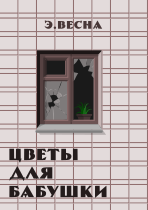
\includepdf[pages={1}]{../images/cover_FlowersForTheGranny.pdf}
\newpage
\thispagestyle{plain}
% ----- FRONT COVER -----

% ------ TITLE PAGE ------
\begin{titlepage}
{
\centering
{~\par}
\vspace{0.25\textheight}
{\LARGE\tofaauthor\par}
\vspace{1.3cm}
{\Huge\textbf{\tofatitle}\par}
\vfill
{
\includegraphics[width=6em]{../images/publisher-logo.pdf}\par}
}
\end{titlepage}

\newpage

% ----- LIBRARY PAGE -----
\thispagestyle{plain}

% ----- CODES BLOCK -----
\begin{minipage}[t]{2em}УДК\\ББК\\~\end{minipage}
\begin{minipage}[t]{0.8\textwidth}\UDK\\\BBK\\\AuthorCode \end{minipage}
% ----- CODES BLOCK -----

\vfill

{\centering\includegraphics[width=0.25\textwidth]{../images/qr-lorem-ipsum.pdf}\par}
\vspace{0.5em}
{\centering\small О книге и авторе\par}
\vfill

% ----- AUTHOR CODE -----
\begin{minipage}[t]{0.05\textwidth}~\\\AuthorCode \end{minipage}
% ----- AUTHOR CODE -----
\begin{minipage}[t]{0.9\textwidth}
\textbf{Весна, Эмиль}

~~~~Цветы для бабушки / Э. Весна. --- \BookVersion. --- Томск: Свободное издательство <<Цунами>>, 2023. --- 222 c.

\vspace{1em}

% ----- ANNOTATION -----
{\small
Россия, 2012 год.
Валерий и Вероника "--- простая российская семья из города Новосибирска.
Как и прочие, они пытаются построить жизнь в медленно набирающей силу политической буре, справляясь с новыми и новыми житейскими трудностями.
Но беда не приходит одна "--- Вероника заразилась неизвестным науке вирусом, само существование которого могло поставить мир на грань катастрофы...
\par}
% ----- ANNOTATION -----

\vspace{1em}

% ----- SECOND CODES BLOCK -----
\hfill \begin{minipage}[t]{0.35\textwidth}{\textbf{УДК~\UDK\\ББК~\BBK}\par}\end{minipage}
% ----- SECOND CODES BLOCK -----

\vspace{2em}

% ----- LICENSE BLOCK -----
{\small
Данная книга распространяется под лицензией \textbf{CC~BY~4.0}.\\
Подробнее: \href{https://creativecommons.org/licenses/by/4.0}{https://creativecommons.org/licenses/by/4.0}
\par}
% ----- LICENSE BLOCK -----

\vspace{1em}

% ----- LICENSE SIGNS BLOCK -----

\includegraphics[width=2em]{../images/cc.pdf}~
\includegraphics[width=2em]{../images/by.pdf}
% ----- LICENSE SIGNS BLOCK -----

\end{minipage}

\newpage

% ----- DISCLAIMER PAGE -----
\thispagestyle{plain}
{~\par}
\vfill
{\centering\Large\textit{Светлой памяти Риты "---\\девочки, которая принимала роды у козы\\и которая кормила меня кексами\\в худшие дни моей жизни.}\par}
\vfill
{~\par}
% ----- DISCLAIMER PAGE -----

\newpage
\thispagestyle{plain}
~
\newpage


\pagestyle{fancy}

\chapter{Трудоустройство}

\subsection{Кошмар}

Вспомните свой самый худший кошмар.

Вспомнили?
Во всех подробностях?

Так вот, это ерунда.

Самый худший кошмар на свете выглядит достаточно безобидно.
Кошмар ограниченного мира.
Вариаций может быть огромное множество, и Варенику сегодня приснилась одна из них.
Звёздное небо, дом с пустыми окнами, занесённый тонким слоем снега переулок и пять могил на обочине.

Важная часть кошмара ограниченного мира --- осознанность и кратковременная иллюзия всемогущества.
Да, я во сне, а значит, всё, что я могу придумать, может стать реальностью!
И только взлетев, распахнув крылья, ощутив биение воздуха в грудь, Вареник понял --- не может.

Далёкие звёзды оказались простыми источниками света, подвешенными в пустоте.
Дом превратился в картонку с прорезями, а переулок --- в единственное во всей этой карманной Вселенной место, где можно стоять и существовать.

Больше там ничего не было.

Вареник спустился к могилам и начал читать надгробия:

\begin{quote}
Владимир Владимирович Шенкерман (1986--2048)

Вероника Андреевна Сафронова-Зима (1989--2072)

Сергей Валерьевич Лебедев (2010--2045)

Маргарита Михайловна Колесникова (2005--2090)
\end{quote}

Последняя могила, принадлежащая <<Валерию Николаевичу Сафронову (1985--2028)>>, была пустой.
Кто-то положил на дно клетчатое одеяло, приглашающе отогнув уголок.

Что, если бы вы не смогли проснуться?

Варенику повезло --- он проснулся.
Могилы и снег сменились теплом постели и живой, невероятно живой жены с огненно-рыжими волосами.
И даже мысль о сходстве карманной и реальной Вселенной его не посетила.
Ему вообще везло --- и с мыслями, и с женой, и с самой жизнью --- как и восьми миллиардам смертных, которым есть куда проснуться и есть куда умереть.

Впрочем, именно сегодня он не чувствовал себя везучим.
На утро было назначено очередное собеседование.

\subsection{Декаданс}

\ml{$0$}
{--- Извините, вы нам не подходите.}
{``I'm afraid you're not right for the job.''}

Стандартная фраза.
Вареник слышал её уже в одиннадцатый раз.
Говорили на собеседованиях разное, но слышал он одно и то же.
Иногда проводивший собеседование эйчар даже начинал извиваться и кривиться, словно змея на сковороде;
Вареник знал --- наступил момент, когда уже всё ясно, деньги отработаны, а желудок требует заслуженной чашки корпоративного кофе.

--- Прощайте, --- коротко ответил Вареник и, собрав свои бумаги, вышел из кабинета.

В этом офисе, как и в прочих других, царил декаданс.
Современные материалы, на поверку оказывающиеся отходами производства.
Запах парфюмерии, сквозь который пробивались ароматы непролеченных язв и убитых алкоголем почек.
Десятки людей с агрессивно-равнодушными взглядами, прячущими страх безработицы, ощущение собственной незначительности и два-три непогашенных кредита.

<<Может, оно и к лучшему>>, --- решил про себя Вареник, ощущая тяжёлый взгляд охранника.
Тот крутил на пальце ключи.
Две тысячи лет назад жил человек, который с точно таким же выражением лица поигрывал кнутом.
Этого не было ни в одной хронике, ни в одном учебнике, но Вареник знал это так, словно видел своими глазами.

<<Прости, Вероника.
Хуёвый у тебя муж>>.

\subsection{Плохое предчувствие}

Предчувствие очередной неудачи преследовало Вареника с утра --- с того самого момента, как он покинул мир с пятью могилами.

Вначале он вспомнил, что его рабочая лошадка, Тойота Королла две тысячи второго года выпуска, стоит в автосервисе, и ехать придётся общественным транспортом.
Затем выяснилось, что интернет закончился в полночь, и узнать дорогу к офису компании можно только у точки бесплатного вайфая в двух остановках от дома.
Наконец, уже настроившись перехватить в кафе пирожок, он выяснил, что забыл в другой куртке карту.
Налички было впритык на дорогу.

Офис находился на возвышенности;
ледяной ветер с Оби забирался под куртку и сбивал с ног.

Охрана сразу встретила его неприветливо.

\ml{$0$}
{--- Я на собеседование.}
{``I'm here for my job interview.''}

\ml{$0$}
{--- К кому?}
{``Who invited you?''}

\ml{$0$}
{<<В смысле --- к кому?>>}
{\textit{What do you mean, ``who''?}}
\ml{$0$}
{В здании находилась только одна компания.}
{There was only one company in the building.}

\ml{$0$}
{--- Щас.}
{``Wait a sec.''}

Вареник выудил телефон и начал искать СМС с данными компании.

\ml{$0$}
{--- Фома Непомнящий, блядь, --- плюнул охранник.}
{``Doubting fucking Thomas,'' the guard spitted.}
\ml{$0$}
{--- Идёт, а к кому --- не помнит.}
{``En route to who-knows-who.''}

\ml{$0$}
{--- Максим Орлов, --- сказал Вареник, проигнорировав реплику.}
{``Maxim Orlov.'' Varenik ignored the guard's words.}

\ml{$0$}
{--- Ну так и звоните ему.}
{``Call him on the phone.''}

\ml{$0$}
{--- До собеседования ещё час, --- сказал Вареник.}
{``I have an hour before the interview,'' Varenik said.}
\ml{$0$}
{--- На улице ветрено, и я думал, просто посижу здесь.}
{``It's windy outside, I hoped I'll just sit here.''}

\ml{$0$}
{--- Здесь вы не посидите, --- обрадовал его охранник.}
{``You won't just sit here.'' The guard definitely tried to make him happy.}
\ml{$0$}
{--- Приходите ко времени.}
{``Come as scheduled.''}

Вареник кивнул и направился к выходу.

<<Охуенное начало охуенной работы>>.

Райончик оказался так себе.
Автострада, автомойки, автосервисы, несколько клиник, пара задрипанных ювелирных салонов и билборд <<Откажись от наркотиков!>>.
Как известно, билборды и надписи на стенах всегда соответствуют местному контингенту.
Ни одного кафе в радиусе километра.

Местный продуктовый был на три четверти заставлен спиртным, одну восьмую прилавков занимали семечки --- ещё один намёк на местный контингент.
Собственно съестное робко ютилось в уголке.
Вареник купил крохотную пачку вафель, чтобы хоть как-то заполнить пустоту в желудке.

Оставшиеся десять минут он провёл в странно современном цветочном магазине, чихая и делая вид, что рассматривает цветы.
Симпатичная продавщица на каждый чих говорила <<Будьте здоровы>> и понимающе вздыхала.

Всё это было зря.

\subsection{Забор и шлагбаум}

Выйдя из офисного здания, Вареник направился к метро.

К станции удалось выйти не сразу.
Дорожная развязка сыграла с пешеходом несколько ей одной понятных шуток, прежде чем милостиво вывела его на нужную улицу.
Вареник обрадовался и рванул через дворы, но радость оказалась преждевременной.
На пути встали несколько новостроек, окружённых глухими заборами;
шлагбаумы стояли, точно крохотные ландскнехты с огромными двуручными мечами.

<<Да какого хрена! --- возмутился Вареник.
--- Как вообще здесь выживать без автомобиля?!
Лабиринт ёбаный...>>

Совсем некстати опять всплыл в памяти утренний сон.

Вареник ненавидел колючую проволоку и заборы с острыми пиками.
Эти вещи --- не просто архитектурные ухищрения, не просто предупреждение;
это настоящее варварство, полное презрение к человеческим страданиям.
Ни одна страна не будет свободной, пока на её территории есть колючая проволока.
В России же даже в городах, предназначенных для проживания свободных людей, каждый второй дом, каждый промышленный или торговый объект ощерились острым металлом, словно зоны.
Пожалуй, единственное, что не имеет границ в России --- стремление возводить границы.

--- Э, сука, куда полез! --- заорал кто-то вдалеке, выбежав из маленькой будки.
Вареник аккуратно перемахнул через шипастое навершие забора, пропустив реплику мимо ушей.

Законы, финансы, политика, военные зоны, частная собственность --- удавки, наброшенные на шею и не дающие сделать вдох ни на миллилитр больше, чем нужно для твоего выживания.
Живи, работай и даже не помышляй выйти за рамки.
И не думай, что эти рамки иллюзорны --- нужно большое мужество, чтобы уйти за границы собственных финансов или привычек.

Ты не можешь построить дом там, где хочешь.
Ты не можешь выращивать культуры и питаться от земли.
Ты не можешь перемещаться по стране, не имея целой кипы бумаг --- документов или валюты.

Вареник желал другого мира.
Но мир только один, что бы ни говорили на этот счёт теории мультивселенных.

...Из-за домов выглянул кусочек оживлённой дороги, а затем показалась и большая красная буква <<М>>.
Философия вылетела из головы Вареника так же быстро, как и появилась.

\subsection{Отголосок бури}

--- Не взяли, --- утвердительно сказала Вероника, едва лицо мужа показалось из-за двери.
--- Иди кушать, через десять минут готово будет.

Вареник повиновался.
Он долго пытался влезть в плисовые штаны и слишком долго рассматривал комично-страшные морды тапочек-драконов.
Подарок Вероники.

--- На, ешь, --- Вероника поставила перед мужем тарелку с овощным супом.
\ml{$0$}
{--- Ты очень грустный.}
{``You look very sad.}
\ml{$0$}
{Тебя обидел кто-то?}
{Did someone hurt you?''}

--- Да нет, --- буркнул Вареник.
--- Просто долго что-то без работы сижу.
И подработок, как назло, нет --- даже грузчики не нужны...

Суп сделал Вареника чуть более разговорчивым.

--- ...Понимаешь, я всё делаю по правилам! --- говорил Вареник.
--- Я выучил все эти стандартные вопросы-ответы на собеседованиях, проговорил, отработал!

--- Верю, --- кивнула Вероника.
--- Только вот...

Она вдруг заулыбалась.

--- Ну чего? --- обиделся Вареник.

--- Да хреновый из тебя врун, зай, --- объяснила жена.
--- Когда ты врёшь, тебя аж перекашивает всего, как будто тебе нанесли смертельную обиду.

--- А, так вот как ты научилась различать, --- буркнул Вареник.
--- Видимо, мне капец.

Вероника нахмурилась и пристально вгляделась в мужа.

--- Ты боишься, что я от тебя уйду?

--- Нет, конечно, --- Вареник улыбнулся, но голос его выдал.

Вероника вздохнула.

\ml{$0$}
{--- Солнце, я знаю, что ты не лентяй.}
{``Sun, I know you're not lazy.}
\ml{$0$}
{Это временные трудности.}
{This is all just temporary.''}

\ml{$0$}
{--- Да какие-то слишком временные.}
{``Too temporary, I'd say.''}

--- Когда я в аварию попала, там вообще трудностям конца-края не было.
Мы это пережили.
Ты меня с ложки кормил, помнишь?

\ml{$0$}
{--- Дело давнее.}
{``Bygones.''}

\ml{$0$}
{--- Именно.}
{``Exactly.}
\ml{$0$}
{Всё это позади.}
{Bygones.}
\ml{$0$}
{А сейчас трудности у тебя.}
{Now it's you who's in trouble.}
\ml{$0$}
{И я буду рядом.}
{And I'm gonna be by your side.''}

Вероника набрала ложку супа и аккуратно поднесла её ко рту мужа.
Вареник усмехнулся и съел предложенное.
По пищеводу прокатилась волна живительного тепла.

\ml{$0$}
{--- Я в тебе засомневался.}
{``I doubted you.}
\ml{$0$}
{Прости.}
{Sorry.}
\ml{$0$}
{Ты обиделась?}
{You feel offended?''}

\ml{$0$}
{--- Нет.}
{``No.}
\ml{$0$}
{Я знаю, каково чувствовать себя беспомощной.}
{I understand what it's like to feel helpless.}
\ml{$0$}
{Засомневаешься в ком угодно.}
{You would doubt anyone.}
\ml{$0$}
{Тогда, в больнице... я каждый день боялась, что тебя не дождусь.}
{That time, in the hospital ... every single day, I was afraid I wouldn't see you again.}
\ml{$0$}
{Что ты умрёшь, встретишь другую женщину, просто решишь, что я тебе надоела.}
{I was afraid you would die, or meet another woman, or just get tired of me.}
\ml{$0$}
{Что я просто останусь одна.}
{I was afraid I would be alone.}
Или, ещё хуже, ко мне начнёт ходить мать со своими вечными разговорами.
\ml{$0$}
{Она грозилась приехать и тебя отвадить, типа, ты уже труп, о душе думать надо, а он тебе голову любовью морочит...}
{She threatened to come and ward you off, like, you're already dead, think of your soul, he's just fooling you with love ....''}

--- Если бы ты мне об этом сказала, я бы её в труп превратил...

--- Да потому и не сказала!
Эта рухлядь и так нам достаточно проблем устроила.

Поев, Вареник повеселел.
Да, безработность --- это неприятно, но, к его счастью, кризис среднего возраста ему пока не грозил.

Вареник отчасти понимал, откуда растут ноги у кризиса среднего возраста.
Всю молодость люди ставят себе какие-то цели.
Школьники должны закончить школу.
Студенты --- закончить универ.
Выпускники --- найти тёпленькое местечко по специальности.
Холостые должны жениться, а бездетные --- завести ребёнка.
И вот, когда все цели достигнуты, в голове человека возникает закономерный вопрос --- а что, собственно, дальше?
Этот вопрос, как контрольный выстрел, добивает окончательно человеческую психику, и без того расшатанную школьными порядками, бессонными ночами перед сессией, орущим дитём и <<работой над отношениями>>.

Отчасти Вареник даже был благодарен судьбе, что его <<победный марш>> оборвался на стадии поступления в универ.
Политех на два года получил хорошего человека, а хороший человек сохранил себе нервы.
Могло быть и хуже.

\asterism

Едва Вареник успел заварить чай, как зазвонил телефон.

--- Варёныч, хай.
\ml{$0$}
{Как здравие?}
{How you feeling?''}

\ml{$0$}
{--- Жив, Киря, твоими молитвами, --- лаконично ответил Вареник.}
{``Alive, Kirya, with the help of your prayers,'' Varenik answered.}
\ml{$0$}
{--- Сам как?}
{``You?''}

\ml{$0$}
{--- Да как-то вот, Варёныч.}
{``Kind of sucks, Varyonych.}
\ml{$0$}
{Короче, ушёл я из <<Ангстрема>>, и Воля ушёл.}
{In short, I retired from Angstrem, and Volya too.}
\ml{$0$}
{По твоим стопам.}
{Following in your footsteps.''}

Голос Кири выдавал его напряжение.

\ml{$0$}
{--- Если ты хочешь занять, не могу помочь, --- предупредил Вареник очевидный вопрос.}
{``If you need money, can't help,'' Varenik prevented obvious question.}
--- Я как уволился, так и без работы сижу.

\ml{$0$}
{--- Бля, братан, --- опечалился Киря.}
{``Sucks, bro,'' Kirya sadly said.}
--- Мож варик какой есть, чтоб по-быстрому?
Лавэ горит, Анька свалить грозится.
Я по кентам посмотрел --- нихуя, у всех напряг.

--- Напиши мне ВКонтакте, я тебе скину кое-что, --- задумался Вареник.
--- Вахтовая работа где-то за Уралом, я такую точно не потяну по здоровью.
Платят немного, но зато вагончик и жратва включены, с голоду не помрёшь.

\ml{$0$}
{--- Заебись!}
{``Fuck yeah!}
Я тебе прям щас маякну!
От души, Варёныч!

--- Говно вопрос, обращайся.

--- Это с твоего склада? --- поинтересовалась Вероника.

--- Ага, --- кивнул Вареник.
\ml{$0$}
{--- Там походу всё.}
{``Looks like they're done.''}

\subsection{<<Ангстрем>>}

Торговая компания <<Ангстрем>> владела складами в нескольких регионах.
Ходили слухи, что её хозяин давно уже перешёл на более выгодный бизнес, перекупив часть акций известных торговых сетей;
склады остались придатком --- малоприбыльным и морально устаревшим.

\ml{$0$}
{--- КОООСТЯ, БЛЯЯЯ!}
{``KOSTYA, MOTHERFUCKER!}
\ml{$0$}
{Опять ты мне, сука, собрал бочку с порохом! --- с этого крика кладовщика Володи начинался рабочий день Вареника.}
{You made a bloody gunpowder barrel, again!'' Every Varenik's day on the job started with that shout of storekeeper Volodya.}

Уже слегка поддатый Костя бормотал извинения и шёл исправлять косяки в сборке.
Ещё совсем нестарый мужик бухал как чёрт две трети жизни.
\ml{$0$}
{Костю увольняли три раза, и три раза он возвращался --- идти ему было некуда, и заменить его было некем.}
{Kostya was fired three times, and came back three times---he has nowhere to go, and there was no one to replace him.}

Киря же, в отличие от Кости, не косячил никогда.
Он кабанчиком метался по складу, молниеносно раскидывая брикеты и связки по коробам.

\ml{$0$}
{--- Ну а хуле, --- говорил Киря прочим, --- хочешь жить --- умей вертеться.}
{``Dafuck'', Kirya used to say to others, ``you wanna live, you gotta spin.''}

\ml{$0$}
{Киря замечательно умел вертеться.}
{Kirya was good at spinning.}
Он получал самую большую зарплату для его должности, его регулярно объявляли работником месяца и выдавали поощрения.
Он имел безусловный авторитет среди мужиков благодаря надёжности и честности.
Работа на складе была его коньком, а должность комплектовщика <<Ангстрема>> --- венцом карьеры.

\ml{$0$}
{Вареник не хотел вертеться --- он хотел жить.}
{Varenik never wanted to spin, he wanted to live.}
Посему же ничем не выделялся среди других.
Ему нравился запах коробок и хруст, с которым они разрывались.
Платили ему гораздо меньше Кири, но тоже неплохо, вовремя --- безусловное преимущество крупной компании.

Вареник сам толком не понимал, почему уволился.
Конечно, он искал работу перед увольнением, за месяц или за два, но попробуй-ка развернуться при графике с двенадцати дня до девяти вечера пять на два.
Отпроситься можно раз в месяц, и то директор косо смотрит.
До этого времени Вареник думал, что такой график специально сделали для того, чтобы мужики не успели набухаться вечером.
Костю, впрочем, это не останавливало --- он активно поддавал уже часа в четыре, запершись в загаженном складском туалете.
И только потом, во время поиска работы, Вареник всё понял.

--- Уходи сейчас, --- сказала Вероника, выслушав мужа.
--- С такими пирогами ты год будешь работу искать.

--- А деньги?

--- Месяц на мою зарплату как-нибудь протянем.

Вероника оказалась права.
Спустя пять дней после увольнения Вареник узнал, что склад влетел на крупную сумму --- больше двадцати пяти тысяч на каждого работника.
Непробитая сборка пропала вместе с фурой, водителем и кое-какими важными документами.
Долг менеджеры милостиво растянули на полгода, не оставляя и тени сомнения в великолепии этого бизнес-плана.

--- Ты всё ещё грустишь? --- спросила Вероника, погладив мужа по голове.

--- Это удивительно? --- улыбнулся Вареник, мешая чай ложкой.
\ml{$0$}
{Чай уже давно остыл.}
{The tea was long cold.}

--- Нет, --- ответила жена.
--- И всё же ты выглядишь счастливее, чем когда ты работал на складе.
Ложись-ка спать, солнц.
Я сегодня ненадолго, вечерком кино посмотрим с пиццей.
На работе шестой сезон Доктора скачала, принесу флэшку.

Вечером позвонил с благодарностями Киря, обещал занести пиво.
Он за полдня устроился на ту самую вахту на вполне достойных условиях.
\ml{$0$}
{Вареник слушал его гоповатую речь в трубке с некоторой завистью.}
{Varenik were listening to his gopnik-like speech on the phone, with some envy.}

<<И почему я так не могу, а?>>

\subsection{Аркада}

Следующее собеседование было назначено на завтра.
Вакансия --- консультант в салоне связи.

На этот раз пришло очень много народа --- молодые и не очень, тёртого вида мужички и такие же ушлые бабы.
Вареник, привыкший к собеседованиям один на один, смотрел на них с удивлением.
Затем пришла милая женщина-эйчар и долго говорила о бонусах, комбо и планах компании.
Правда, её глаза светились чем-то непонятным --- не усталостью, не скукой, а скорее полной тревоги грустью.
Видимо, у неё тоже был план, который следовало выполнить.

После наступило время самопрезентации.
Тёртые мужички и ушлые бабы разом превратились в нежных овечек, уверяя девушку, что они будут самыми спокойными и продуктивными работниками.
Вареник тем временем прокручивал в голове услышанные цифры.
Вскоре, отчаявшись найти у себя способности к математике, он вышел в коридор и позвонил лучшему другу, Владимиру Шенкерману.

--- На хуй, --- сразу сказал Шенкерман.
--- Платить тебе будут копейки.
Двойная премия выплачивается за перевыполнение плана, то есть сразу урезай все бонусы вдвое.
Кроме того, целых десять пунктов, связанных между собой какой-то хитровыебанной связью, про которую она вам ничего не сказала!
Не, Вареник, лучше вали оттуда.
Это игра с неизвестными правилами, ты однозначно проиграешь.

--- Да крупная же вроде компания! --- возражал Вареник.
--- Говорят, их вообще какие-то друзья Путина выкупили...

--- Серьёзные дяди устанавливают нормальную базу, а не устраивают аркаду с бонусами.
\ml{$0$}
{Она сказала тебе размер базового оклада?}
{She tell you the amount of basic salary?}
\ml{$0$}
{Сказала?}
{Did she?''}

\ml{$0$}
{--- МРОТ.}
{``Minimum wage or so.''}

\ml{$0$}
{--- Умножь его на два, если ты хороший работник.}
{``Multiply that by two if you're a good employee.}
\ml{$0$}
{Умножь его на полтора, если ты хороший работник, а на дворе две тысячи двенадцатый год и кризис.}
{Multiply that by one and a half if you're a good employee, and now is two kay twelve and the world economic crisis.}
\ml{$0$}
{Вот твоя зарплата.}
{That's your salary.''}

--- Ты думаешь, что кризис есть на самом деле?

--- Какая разница, есть он или нет?
Важно, что о нём говорят.
Уровень твоей зарплаты зависит от трепла в телевизоре, а не от невидимой руки рынка.

Вареник извинился перед девушкой-эйчаром и ушёл, не дождавшись своей очереди.

\subsection{Шенкерман}

--- Хочешь прикол?

--- Ну?

--- Я в анкете в графе <<имя>> написал <<Вареник>>.

--- Бля-я, --- весело откликнулся Шенкерман.
--- А как тебя всё-таки звать?

--- Володь, ты издеваешься?

--- Я серьёзно, --- голос Шенкерман звучал слегка растерянно.
--- Сколько тебя помню, ты всегда был Вареником.
А кто ты по паспорту-то?

--- Валерий.
Валерий Николаевич.

--- Ты потратил пять секунд на то, чтобы вспомнить, --- заметил Шенкерман.
--- Как прозвище-то въедается.

--- Неправда.
Ты меня просто ошарашил вопросом.

--- А давно тебя по имени-отчеству?

--- А вот хер бы знал.
В политехе вроде.
У нас препод был смешной, всех звал <<мастерами>>.
Я был у него <<мастер Сафронов>> или <<Валерий Николаевич>>.

--- Он тебе шанс давал, Вареник, --- ухмыльнулся Шенкерман.

--- Какой шанс?

--- Недостаточно родиться Валерием Николаевичем.
Им надо стать.

Владимир Шенкерман был другом Вареника с ранней юности.
Кажется, они учились на одной параллели, но прочие подробности их знакомства терялись в сумраке веков.
Да и какая разница --- была это какая-то школьная пьянка, жили ли они в одном дворе или просто столкнулись в коридоре?
Разницы нет никакой.

Нельзя сказать, чтобы их связывали какие-то общие интересы.
Это была чистая дружба, основанная лишь на совместном (порой горьком) опыте.
В пользу этой дружбы говорило одно --- она была, и она была долго.
С прочими друзьями Вареник общался ровно до того момента, пока с ними было о чём покурить;
последняя сигарета истлела года два назад.

Шенкерман был, по представлениям Вареника, <<серьёзным человеком>> --- он работал девелопером в небольшой, но неплохо зарекомендовавшей себя фирме.
А ещё Шенкерман, по выражению Вареника, умел <<делать деньги из воздуха>>, то есть занимался фрилансом.
Самому Шенкерману эта фраза очень не нравилась.
Он много раз объяснял другу, что клиентов искать не так просто, что фриланс оплачивается по часам, что для фриланса нужна самодисциплина и жёсткий распорядок дня, но все эти доводы игнорировались;
концепцию тайм-менеджмента Вареник понимал очень прямолинейно, использовал её не более одного-двух раз в день, а потому не видел в грамотно составленном личном расписании никаких особенных заслуг.

Примерно так же, как Варенику не везло с работой, Шенкерману не везло в личной жизни.
Он знал, каким концом нужно тыкать в девушку букетом, он знал несколько достаточно оригинальных комплиментов, но это почему-то совсем не помогало.
Теми же, кто очевидно зарился на его достаток, он брезговал.

Впрочем, отношения у Шенкермана были --- и даже длительные.
Однажды он разрывался аж между двумя девушками;
Варенику даже пришлось вмешаться, пока в дело не встрял алкоголь.
Всегда готовый разрулить любую ситуацию, Шенкерман был абсолютно беспомощен перед девушками и вином.

--- Вот чем тебе нравится Светочка? --- допытывался Вареник во время очередного сеанса психотерапии.

--- Светочка хорошо готовит, с ней есть о чём поговорить, --- отвечал Шенкерман после некоторого раздумья.

--- А Олечка?

--- Олечка картавит, --- не задумываясь выпаливал влюблённый.

Вареник тяжко задумывался и замолкал.
Видимо, в представлении Шенкермана картавость если и не перекрывала все достоинства Светочки, то по крайней мере могла составить им серьёзную конкуренцию.

Светочка всё же выиграла соревнование с небольшим перевесом.
На целых два года Шенкерман выпал из эволюционного процесса.
Обстоятельств, по которым они разошлись, Вареник так и не узнал;
Шенкерман начинал плеваться при любом упоминании имени <<Света>>.

Тем не менее, Шенкерман обнаруживал неожиданную мудрость, когда речь шла о чужой личной жизни.
Веронику Вареник выбрал благодаря ему.
Как-то в Новый год они затусили с компанией девушек-биологов, и Вареник положил глаз сразу на троих.

--- Что скажешь? --- шепнул он другу, поделившись наблюдениями.

--- Бери рыжую, --- не задумываясь ответил Шенкерман.
--- Счастливые стригутся коротко.

В первый же год отношений Вероника отпустила кудри.
Оказалось --- ждала нужного человека.

\subsection{Старые связи}

Работа нашла Вареника неожиданно.
Он случайно зашёл в кафе-столовую неподалёку от дома;
сети обслуживания <<С пылу с жару>> требовались сотрудники.

--- Да мы вас знаем, вы же к нам с женой регулярно ходили в прошлом году! --- радостно сказала менеджер.
--- И девочки вас тоже помнят.
Приходите завтра, пара дней стажировки --- и мы вас устраиваем.

\subsection{Бритьё}

Первый рабочий день --- это не просто день.
Это ритуал.
С сегодняшнего дня начинаем новую жизнь, и она лучше, чем прежняя.

Встать за пять минут до будильника.
Поцеловать ещё спящую жену.
Не удержавшись, уткнуться носом в спутанные волосы, издающие сладкий карамельный запах.

Пописать.
Вареник сел на унитаз, раздвинул ноги и наклонился вперёд, нацеливая скованный стояком член куда надо.
Он быстро обучился писать сидя, пока их с Вероникой мотало по крохотным съёмным конуркам.
Отличный способ, никаких брызг, но как же хорошо, что этого никто не видит...

Умыться, почистить зубы и побриться.
Закончив манипуляции с щёткой, Вареник набрал полный рот ополаскивателя и аккуратно выплюнул его в раковину.
Затем достал из футляра бритву, нанёс на щетинистое лицо немного пены и сделал первый мазок.
Щетина скрипела и трещала, и это каждый раз доставляло Варенику какое-то странное удовлетворение --- словно от покоса травы в деревне.
Из зеркала смотрело немного опухшее, но привлекательное мужское лицо с раздвоенным подбородком.
Под нависшими седеющими бровями мягко светились голубые глаза, обрамлённые едва заметными тёмными мешками.
Чуть ниже шли мощные плечи, подкаченный грудак --- предмет гордости --- и небольшой округлый живот, покрытый чёрными волосами.
Варенику нравилось смотреть на себя в зеркало, но он никогда не сказал бы этого вслух даже жене.
Просто есть вещи, о которых не стоит говорить.

--- Зай, ты чего так долго?

--- Какаю, солнц.
Пару минут.

Спустя пару минут раздавался маскировочный звук смыва.
И мысль:
<<Жаль, что зеркало только одно>>.

Упражнения.
Вареник расстелил на кухне коврик, принялся отжиматься, качать пресс и спину.
Вдох, выдох, вдох, выдох, два подхода.
Мышцы болезненно трещали, словно пучки корабельных канатов, и это тоже ему нравилось.
Личный рекорд --- сорок два отжимания, но обычно за подход он делал около двадцати пяти --- тридцати.
Не ахти, зато своё.

Завтрак.
Чашка крепкого растворимого кофе, четыре кусочка колбасы, четыре тоста с маслом (Вареник и Вероника обзавелись дешёвым тостером, как только съехались).
Чтобы не разбудить жену (или, что гораздо хуже, соседку) щелчком тостера, Вареник плотно закрыл дверь на кухню.

Ключи от дома.
Ключи от почтового ящика.
Ключи от машины.
Машина привычно отозвалась снаружи дома.
Пусть прогреется.

Надев куртку, Вареник аккуратно приоткрыл две скрипучие двери и, не доверяя шумному защёлкивающемуся замку на железной двери, закрыл замок ключом.

\subsection{Ревность}

Так для Вареника началась новая жизнь, полная жратвы и адреналина.
На его взгляд, сочетание было идеальным.

Жратву Вареник ценил, особенно вкусную.
Наверное, это приходит к любому, кто хотя бы два месяца жизни сидел на крупах.
Или две недели лежал в реанимации с назогастральным зондом.
Приверженцы диет редко знают лицо настоящего голода.

--- Так, что за дела? --- возмутилась Вероника, когда муж впервые отказался вечером от супа.
--- Ты любовницу завёл, засранец?

Вареник в общих чертах объяснил, что в перерыве между работой --- разливанием соков, перетаскиванием гастр и превращением продуктов в различного рода геометрические тела --- он был занят исключительно перекусами, и для супа места просто не осталось.
Жену объяснение не устроило.

--- Да не с кем мне там изменять! --- развёл руками Вареник.
--- Ты ж помнишь то кафе, там работают одни пончики!

--- Весьма милые пончики, между прочим!
С сахарной пудрой!

--- Ну да, милые.

--- Ясно.
Развод и девичья фамилия.

Периодически Вареник и Вероника играли в ревность.
Но без души, без чувства.
После нескольких лет совместных скитаний, безденежья, ссор с родственниками и друзьями настоящая ревность кажется чем-то ребяческим и глупым.
Примерно как новомодные диеты.

\subsection{Коллектив}

Коллектив попался хороший.
Наверное, потому что сытый.
Люди очень часто несчастны лишь потому, что плохо питаются.

--- Всему научим, бля, --- грузно ворковала повариха Маша.
--- На подхвате, нахуй, поработаешь --- и на раздачу.
Ебало у тебя презентабельное, язык подвесим.
Народ здесь заебись, чётенький.
Только академовские, блядь, часто залетают, тут пересадка недалеко.
Студенты, профессора, бля.
Сложно с ними, Вареник, ох ебать сложно...
Я блядь-нахуй ващще порой не въезжаю, как с ними перетирать.

Раздача пошла бодренько.
Вареник внезапно обнаружил в себе незаурядный талант к общению с людьми.

--- Идиоты! --- орали с раздачи поварам.

--- Внутри каждого идиота скрывается личность! --- неожиданно глубокомысленно парировали с кухни.

Вареник немедленно нанёс изречение на лист бумаги и повесил на вытяжку, прямо над своим рабочим местом --- разумеется, в зоне видимости только себя.
С тех пор оно помогало ему общаться даже с самыми неприятными клиентами.
Впрочем, внезапно прибывшее начальство распорядилось снять пакостную бумажку --- видимо, не оценило глубину мысли.
Или оценило.

\textspace

--- Жратва --- это, конечно, здорово, --- скептически сказал Шенкерман.
--- Но что там кроме этого?
Карьерный рост, деньги?

--- Я рад и тому, что есть, --- ответил Вареник.

--- Сколько в месяц?

--- Двадцать.

--- Вареник, --- проникновенно сказал Шенкерман, --- это копейки.
Ты же не собираешься останавливаться там навсегда?

--- Нет-нет, --- заверил Вареник, перед мысленным взором которого всё ещё висел большой запечённый бутерброд...

Трудностей работа почти не вызывала.

--- Серьёзно, почти как на складе, только без тяжестей.
Единственная поебота с паспортами качества --- там регулярно проходят проверки.
Приходится писать на завтрашнее число с вечера.

--- Паспорта с завтрашним числом?
На продукты?

--- Ну да, --- ухмыльнулся Вареник.
--- А что?

--- Да ничего, --- буркнул Шенкерман.
--- Просто ты как-то чересчур легко говоришь о том, что являешься соучастником преступления.

Вареник поперхнулся и сменил тему.

\chapter{Благотворительность}

\subsection{Жена}

Существует забавная теория о громоотводах.
У человечества есть громоотводы ненависти, к коим, безусловно, любил относить себя Шенкерман --- всякий раз, когда его называли <<жидопидарасом>>, что случалось явно чаще честных президенстких выборов в России.
Вареник скептически относился к словам приятеля, но в существование громоотвода грусти поверил бы без лишних слов.
Одним из них была Вероника, и судя по объёму грусти, который она успешно утилизировала, Земля не утопала в печали благодаря не более чем десяти столпам.

Вероника работала в <<Векторе>>, новосибирском центре вирусологии и биотехнологии.
Вареник мало знал о том, чем именно занимается жена;
она предпочитала не распространяться.
Гораздо больше Вероника рассказывала о коллегах --- у кого какие проблемы, кто как живёт.
По-видимому, тихая и чуткая девушка служила на предприятии нештатным психологом --- ей рассказывали всё, от подробностей рождения до самых страшных личных тайн.
Иногда после очередного сеанса психотерапии Вероника приходила домой хмурая, и Вареник знал --- столп Земли нужно поддержать.

--- Опять передозировка? --- шутил он, обнимая жену перед сном.

Вероника поглубже зарывалась носом мужу в подмышку и молча засыпала.
Наутро всё как рукой снимало;
а вот Вареник мучился кошмарами целую неделю и мысленно благодарил небеса, что эту странную роль --- роль громоотвода --- Судьба назначила не ему.

\subsection{Благотворительность}

--- Солнце, --- позвала Вероника.
--- Ты занят?
Тут из <<Незнайки>> новое задание пришло.

--- Где моя футболка с Суперменом?! --- тут же отпустил дежурную шутку Вареник.

Вареник очень любил благотворительность.
Ему давно уже хотелось завести детей, но регулярно возникали какие-то проблемы --- наподобие недавнего увольнения.
Объявления о сборе средств на лечение детишек печалили его, а порой и приводили в ярость.

--- Опять мошенники, блядь, суки ёбанные, --- плевался он, увидев очередной пост ВКонтакте.

Но год назад ему удалось-таки найти в Новосибирске настоящую благотворительность.
Малоизвестный фонд <<Незнайка>>, основанный энтузиастами из Академгородка, оказался достаточно прозрачным и надёжным --- в частности, он никогда не собирал пожертвования деньгами.
Интересы у фонда были достаточно широкие --- он помогал детским домам, ветеранам войн, инвалидам и многодетным семьям.

Вероника относилась к затеям мужа достаточно скептически --- до первых заданий.
Вскоре супруги стали постоянными волонтёрами фонда.
В конце концов, почему бы и нет.

--- Ну что там? --- спросил Вареник, поцеловав жену в щёку.

--- Всероссийская благотворительная акция <<Цветы для бабушки>>.

--- Для кого?

--- Для бабушки, зай.
Читай.

Вареник пробежал глазами электронное письмо.

--- Ясно.
Футболка отменяется, старушки юмор не оценят.

--- Берём?

--- Ну конечно.

\subsection{Сидр}

--- Название какое-то странное, --- критически заметила Вероника, вытаскивая лифчик через рукав футболки.
--- <<Цветы для бабушки>>.
Как будто всё, что сейчас нужно бабушкам --- это цветы.

--- Я сам так же подумал.
И не я один.
Я сегодня звонил в <<Незнайку>>.
Волонтёры предлагали доставить продукты, починить технику, всякое такое.
Организаторы акции наотрез отказались.
Цветы --- и точка.
<<Запросы составлялись с учётом мнения бабушек, бабушкам от вас ничего, кроме внимания, не нужно>>.

--- И бабушки странные, --- продолжала Вероника.
--- Нетипичные.
Обычно они так и норовят что-то ухватить, нужное-ненужное --- плевать.

--- Может, эти совсем старые, при царе выращенные, --- пошутил Вареник.
--- Ладно.
Машину я заправил.
Ты отпросилась на завтра?

--- Ага.
Давай заодно после бабушек в Икею завернём.
Нужно полочки купить, коврик и полотенца.

--- И сидр.

Вероника расплылась в улыбке.

--- И сидр.
Грушёвый.

--- Может, я тебе всё-таки нормальный куплю, с алкоголем?

--- Нет.
И не смей при мне называть ненормальным икеевский сидр.

\subsection{Дорога}

Вероника уже давно спала, откинув голову на сиденье и открыв рот.

--- Слушай, вот зачем тебе это понадобилось, а? --- сонным голосом спросил Шенкерман.
--- Я не выспался...

--- А я тебя предупреждал, что завтра едем.
Цветы не помн\'и.

--- Ладно, ладно!

Уже на трассе Вареник вспомнил, что забыл посмотреть адрес.

--- Так, третий поворот должен быть.

--- А куда мы едем, если конкретно?

--- Зеленообск, улица Фрунзе, шестнадцать.

--- Ты прикалываешься?

--- В смысле?

--- Какой нахуй Зеленообск?
Может, Краснообск?

--- Володя, не знаю как ты, а я в Новосибе живу с рождения.
По-твоему, я не знаю, где Краснообск?

--- Так ты серьёзно?

--- Да, блядь, серьёзно.
Зеленообск, Новосибирская область.
Да, я тоже слышу о нём в первый раз.
Третий поворот на трассе, потом по просёлочной дороге десять кэмэ и направо.
Глянь на карте, где Фрунзе, шестнадцать.

--- Я телефон не взял, --- пожаловался Шенкерман.

--- Молодец, подготовился.

Вареник вытащил свой.

<<Критическое обновление.
Пожалуйста, подождите, установка может занять...>>

--- Сука, да вы издеваетесь.

--- Что ещё?

--- Обновление, мать его.
Вообще нужно спрашивать мнение пользователя, удобно ли ему...

--- Да кому всралось твоё мнение?
У Гугла бизнес-план горит.
Надо же поскорее напихать в твой кирпич ещё больше трекеров, рекламы и прочего говна.
Гугл --- он как моя мамаша придурошная: понимает с полуслова, но лезет куда не просят!

Вареник громко выругался и забросил телефон в бардачок.

--- Нику будить?

--- Она смартфон редко носит.
У неё раскладушка, древняя как говно мамонта.
Ладно, хуй с ним, может, взяла...
Ника!
Солнце ты моё!
Телефон твой нужен!

Ответом был короткий грудной всхрап.

--- Мда.

--- Давай я у неё в кармане пошарю, --- предложил Шенкерман.

--- Так, блядь, никакой акробатики у меня в машине!
Тем более на трассе!

--- Что за шум, а драки нету? --- сонно осведомилась Вероника.

--- Карту на телефоне открой, солнц.

--- Я звонилку только взяла, зай.

--- Ладно, спи дальше.

--- Ну и хуле делать тогда? --- поинтересовался Шенкерман.

--- Хуле делать?
По старинке будем действовать --- останавливаться и спрашивать людей.

--- Кого мы встретим в восемь часов утра, в воскресенье?

--- Таких же дебилов, как и мы, Володька, только с работающими, блядь, телефонами.

--- Я надеялся, что ты скажешь <<Повернём назад и поедем досыпать>>.

--- Не дождёшься.
Букеты уже купили, блин.
Поздно уже, сука.

--- Какая гадость эта ваша благотворительность.

--- Заткнись, а?

Вареник дёрнул коробку передач и раздражённо вдавил педаль газа.

\subsection{Атлас}

--- Вареник, --- осторожно начал Шенкерман.

--- Что, Володя? --- Вареник говорил преувеличенно-ласково;
руки сжимали руль до характерного хруста.
Это был восьмой круг по дорогам Зеленообска в поисках прохожих.

--- Я тут в бардачке нашёл карты автодорог.
Семьдесят пятого года.
Кажется, я знаю, куда ехать.

--- Отцовский, --- хмыкнул Вареник, бросил взгляд на карту и вывернул руль.
--- Он всегда ездил по этому атласу.
Мудрый был человек.

--- Блядь, тут темно как в жопе негра.
Они вообще фонари включают?

--- Типичный зажопинск, --- пропыхтел Вареник.
--- Ни освещения, ни нормальных дорог.
Даже указателя на трассе нет...

Шенкерман промолчал.
Он уже успел заметить в слабом свете зари дома-пустышки за разросшимися обломанными тополями.
Не особо похоже на типичный зажопинск.

\subsection{Проводница}

--- Спасибо, Раиса Семёновна, --- поблагодарил Вареник.
--- Без вас мы бы точно не нашли...

--- Да я так и подумала, --- затараторила старуха.
--- Дай, думаю, встречу.
Думаю, чай, не доберуцца.

--- Ого, --- Шенкерман пнул на дороге что-то, оказавшееся самодельным противоавтомобильным ежом.
--- От кого защищаетесь, Раиса Семёновна?

--- Да какие защиты, родненький.
Чай, отсохла досочка с гвоздиками.
Чай, лежит.
Дворников-то нету у нас...

--- Ну-ну, --- буркнул Шенкерман себе под нос.
--- Как удачно упала досочка с гвоздиками, что, езжай мы прямо к общаге, в эту досочку бы и вляпались.
А вот и ещё одна, только на этот раз присыпанная песком...

--- Володя, хватит нудить, --- Вареник явно нервничал.
--- Прояви уважение.
Потом расскажешь, если что-то не нравится...

Они миновали упавшее дерево, и перед ними предстала во всей красе старая советская общага, обшитая фигурной бетонной плиткой.
В отличие от окружающих домов, в ней были целые стёкла.
Между окнами повисли верёвки, полные сушащегося белья.
Кажется, кто-то наверху стирал прямо сейчас;
из окна доносилась музыка:

\begin{quote}
Толка вэтэр буйны паёт за ка-армои,\\
Чио-чио-сан, я хачу быт с та-абои.\\
Толка волны бьутса а бэрэг кру-утои...
\end{quote}

Музыка на секунду застопорилась и продолжила уже женским голосом:

\begin{quote}
И-иии лихо-ой\\
Ветер гонит их за мно-ой...\\
О-ооосень, осень,\\
Ну давай у листьев спросим,\\
Где он, май, вечный ма-ааай...
\end{quote}

--- Саня, --- гулко рявкнула Раиса Семёновна на весь двор.
--- Убери эту какофонию, не позорься.

Музыка тут же утихла, сменившись плеском воды.

--- Простите, родненькие, --- затараторила Раиса Семёновна.
--- Любит она эту новомодную музыку, даже манитовон приташшила.
С барталейкой манитовон.

--- Всё хорошо, --- успокоил старушку Вареник.
Шенкерман и Вероника тихо давились от смеха.

\subsection{Туалет}

Вдруг Вареник понял, что ему срочно нужно в туалет.

--- Извините, --- понизил он голос, --- мне бы это...

--- Пошли, --- улыбнулась старушка.
--- Бумажка нужна?..

Она ушла в другую комнату и вернулась с кипой пожелтевших от времени бумаг.

--- Держи.
Сортир снаружи, у того зелёного здания.

--- Вот спасибо, --- обрадовался Вареник и махнул Шенкерману, чтобы тот подождал.

\subsection{Дорога обратно}

--- Это что? --- поинтересовалась Вероника, показывая бумаги.

--- Это мне бабушки дали, чтобы я в туалет сходил, --- объяснил Вареник.

--- Ну ничего себе, --- возмутилась Вероника.
--- Это чей-то дневник был, ты в курсе?
Ты подтёрся чужим дневником, гад.

--- Ну извините, рассматривать у меня времени не было, мысли были заняты другим! --- съязвил Вареник.
--- Что за дневник-то хоть?

--- <<Костомарова З.\,П., вторая Восточно-Саянская экспедиция, 1929 год>>.

--- Да ёжкин, я думал, школьный дневник.

--- Нет, точно не школьный, --- Вероника заулыбалась и пролистала дневник.
--- Ух ты, тут <<яти>> машинописные.
Дореволюционная грамматика.
Впервые вижу машинописные <<яти>>, такое вообще в природе существует?

--- Может, подделка, --- предположил Шенкерман.

--- Не похоже.
Тут даже бумага какая-то... другая какая-то бумага.
На ощупь другая.
Зай, слышишь?

--- Ну ясно.

--- Что тебе ясно, солнце? --- раздражённо буркнула Вероника.
--- Дневник из экспедиции, почти столетней давности.
По-твоему, нормально этим подтираться?

--- Ваще зашибись.
Жопа помолодела лет на десять.

--- Зая.

--- Ник, они мне его сами дали.

--- И? --- голос Вероники опасно повышался на каждой фразе.

--- Давай я съезжу в следующую субботу, верну его и извинюсь, хорошо? --- устало сказал Вареник.
--- Я не хочу снова ехать через эту пробку.

--- Вот так бы сразу.
Но вначале я его прочитаю.

--- Договорились.

\subsection{Постоянное}

Шенкерман зашёл помыться и с омерзением оглядел общую ванну.
Жившая у соседей старуха, очевидно, подмывалась и не убрала за собой.
Ванну Шенкерман помыл, но плавать в растворе чужого дерьма, пусть и гомеопатическом, ему не хотелось.
Он наскоро принял душ, стараясь стоять на самом конце ванны, который едва заливала вода.

--- Слушай, --- спросил он у Вареника, --- ты не думаешь переезжать?

--- Куда?

--- Неважно куда.
Ты мне недавно жаловался, что детей всё не завести --- то одно, то другое, то третье.

--- И что?

--- Дети --- это последнее, о чём можно мечтать в такой хибаре.
В конце концов, работа у тебя сейчас есть, поищи вариант получше.

--- Это был временный вариант после того, как нас с Никой выкинули на мороз, --- извиняющимся тоном сказал Вареник.

--- И вы уже полгода здесь, --- подытожил Шенкерман.
--- Нет ничего более постоянного, чем временное.

--- Я вообще не знаю, готов ли я к детям.

--- Ты поймёшь, когда будешь готов.

--- Звучит охуенно мудро, Володь, но лёгкий оттенок <<отъебись>> портит всё впечатление.

--- Нет здесь никакого оттенка.
Ты реально поймёшь, когда придёт время.

--- Не представляю, как это может быть.

--- Я иногда помечтать любил, --- сказал Шенкерман.
--- В шараге особенно.
Знаешь, воображал себя мегакрутым воином или что-то подобное, когда типа раздеваешься до пояса и идёшь ломать руки-ноги.
И вот однажды лежу я себе, мечтаю.

--- Бля, а можно на этом закончить?

--- Нельзя.
Мечтаю я, говорю, перед сном.
Зима, снегопад, толпа народу.
И выходит против меня такой громила.
Я таких больше всего боялся --- кого свалить у меня тупо силёнок не хватит.
Раздевается громила до пояса, мышцами играет, насмехается надо мной.
А я, вместо того, чтобы тоже раздеться, надеваю шапку и заправляю свитер в штаны.
Зима же, снегопад.

--- И к чему это?

--- Да так, --- ухмыльнулся Шенкерман.
--- Я просто в тот момент понял, что повзрослел.

\subsection{Несуществующий город}

--- А прикол в том, что города этого ни на картах нету, ни в справочниках! --- Шенкерман развёл руками.

--- Ты уверен, Володь?

--- Зайди в Гугл Мапс!
Какой в жопу Зеленообск?
На этом месте лес и голая трасса, ни поворота, ни города!

--- Напиши в техподдержку.
Не может быть.
Помнишь атлас, по которому мы ехали?
Семьдесят пятого года, да?

--- Сейчас два ноль двенадцатый.
И Гуглю я доверяю больше, чем твоим совковым картам.
Те малость устарели.

--- Но ты же сам мне его нашёл на карте, Володька!

--- Мало ли что я нашёл спросонья, --- буркнул Шенкерман.
--- Не мог целый город, вот так взять и испариться.
Значит, либо мы были в другом месте, либо... на этом мысль останавливается.
Ну сам подумай, --- мы у кого-то спросили название города?
Нет.
Мы в диком недосыпе приехали утром, зашли к бабушке, подарили цветы.
Всё, блядь.

--- А адрес?
Улица Фрунзе, дом...

--- Вареник, не тупи.
Улица Фрунзе бывает везде.

--- Да, точно, сорян.
А почему все были в курсе, что мы приедем?

--- А откуда я знаю?
Акция всероссийская!

--- Но...

--- И последнее, Вареник, подожди.
Сколько человек должно было приехать в этот день?

--- Около десяти.

--- А сколько было?
Ты, я и Ника, всё!

Вареник был вынужден признать, что друг прав.
Мистики ноль.
Они просто ранним утречком приехали неизвестно куда и подарили цветы неизвестно кому.
На этом его тревоги закончились.

Для Шенкермана они только начались.
Приехав домой, он раз за разом в мыслях возвращался к душераздирающему пейзажу, который встретил их в Зеленообске.
Дома-<<пустышки>>, поросшие бурьяном бетонные плиты на дорогах, отсутствие неоновых вывесок и вообще какого-либо освещения.
Отсутствие прохожих, наконец.

Подобное запустение было чем-то из ряда вон выходящим, даже для России.
Этот город мог существовать на Курилах, в якутской тайге или ином Богом забытом месте.
Но не в центре Новосибирской области.
Шенкерман несколько раз проверил карту уже дома --- ничего, даже на спутниковых снимках.

<<Ну уж спутник-то их должен был увидеть, --- думал он.
--- Впрочем, я даже не помню, в какую сторону мы ехали.
Здесь сворот, это точно, панораму узнаю, но дальше...
Даже дорога не отмечена.
Разброс десять километров.
И хорошо, если десять, Вареник на нервах был, я сонный, могли и тридцать накатать.
Вот тут какая-то деревня, и вот тут, и даже близко не похоже.
Нету здесь Зеленообска.
Нету>>.

Впрочем, возложенная фондом миссия была успешно выполнена, и новоявленный Сайлент-Хилл забылся за чередой обычных забот.

\chapter{Переезд}

\subsection{Коллекторы}

<<Бля.
И камеру-то не вытащишь --- выбьют сразу из рук...
Зараза>>.

--- Я тебя не спрашиваю, вступал ты в наследство или нет.
Предупреждаю, пока по-хорошему: покрой задолженность.
Если заплатишь в срок --- жена будет цела и ты будешь цел.

--- Понял я, понял, --- буркнул Вареник, высвобождая руку.
--- Хватать меня необязательно.

--- Я надеюсь, что понял, --- ухмыльнулся камушек.
--- Бывай.
Заплатишь долг --- авось и не свидимся.

Мужчины повернулись и зашагали по направлению к центру.

--- Э, мужики, --- окликнул их Вареник.
--- Вы обронили.

Камушек обернулся и, увидев в руке Вареника красную обложку паспорта, похлопал себя по карманам.
Второй сделал то же самое.

--- Благодарствую, --- камушек уже сделал шаг по направлению к Варенику, как тот припустил со всех ног.

--- Э, СТОЙ, СУКА!

<<Так, супер за углом, там камеры...
Телефон, разблокировка, камера, нагрудный карман, глубина которого как раз позволяла оставить камеру открытой...>>

Хлоп --- и по стенам запрыгал шарик от травматического пистолета.
Вареника пробил холодный пот.

<<Бля.
Скорее, скорее на людное место!..>>

\asterism

--- Да мой это паспорт, мой, --- убеждал Вареник.
--- Вы ж меня обыскали, другого при мне и не было.
А эти мужики меня убить хотели.
Выстрелы и угрозы слышно на записи.

Молодой черноглазый сержант вздохнул и прикрыл лицо рукой.
После того, как выяснилось, кто есть кто, ему, как самому молодому по возрасту и по званию, поручили самую грязную работу --- <<нянькаться с терпилой>>.

--- Должник?

--- Нет, --- повторил Вареник.
--- У матери долги были, но поручителем она меня не писала, а я в наследство не вступал и не собираюсь.

--- Заявление писать будете?

--- Буду.

\asterism

--- Оглядывайся, королева армянская, --- прошипел один из них.
--- Мойкой распишу и тебя и суку твою, слово пацана!

--- Закройся, дырявый, --- буркнул Вареник.

--- КТО ДЫРЯВЫЙ? --- коллектор завыл и задёргался, словно в припадке.
Наручники звякали и скрипели о решётку.
--- КТО ДЫРЯВЫЙ?
ТЫ КОГО ДЫРЯВЫМ НАЗВАЛ?
ОТВЕТИШЬ ЗА ДЫРЯВОГО!

Вареник поморщился и закрыл дверь, пока снаружи нёсся всё тот же мотив на высоких нотах:

--- КТО ДЫРЯВЫЙ?
КТО ДЫРЯВЫЙ?

\asterism

--- Валерий Николаевич, --- сержант был явно веселее.
--- От лица нашего отдела хочу вас поблагодарить.

--- Что такое? --- насторожился Вареник.

--- Ничего плохого для вас и для нас, --- успокоил его сержант.
--- Калгин уже был в федеральном розыске, а Шишкин проходил подозреваемым по сто пятой с отягчающими, пункт <<З>>.

--- Напомните, что это за статья?

--- Убийство из корыстных побуждений, а равно сопряженное с разбоем, вымогательством или бандитизмом.
Кстати, тоже с использованием травматического оружия.

--- Ого, --- Вареника снова пробил холодный пот.

--- Мы их сразу отправим куда следует, а вы, скорее всего, пойдёте свидетелем.
Вас пригласят позже.
Но я, от себя, то есть от своего имени, такскть, хотел бы вас предупредить...

--- О чём?

--- У вас жена есть, --- сказал сержант, понизив голос.
--- И дети, наверное?
Вам стоит сменить место жительства.
На всякий пожарный.
Ненадолго, на несколько месяцев, может, снять жильё где-нибудь.
Просто, такие времена, и мы, к нашему, такскть, стыду, вряд ли сможем обеспечить вашу безопасность.

--- Вы думаете, что мне могут отомстить?

--- Следствие в процессе.
Пока могу лишь дать вам совет.
Калгин, скажем так, настроен серьёзно.
Повторяю, это от меня, то есть от моего имени лично совет.
У нас просто были уже случаи...

--- Ничего, --- быстро сказал Вареник.
--- Мы всё равно собирались переезжать, вот и повод появился.
Спасибо вам большое, Алексей Леонидович.

--- Можно просто Алексей, --- сержант пожал Варенику протянутую руку и указал на выход.
--- Вот ваш пропуск.

\asterism

--- В общем, зай, мне повезло, --- закончил Вареник, прихлёбывая овсянку.
--- Тупо повезло, что за углом был отряд ОМОНа, которые перед захватом зашли купить сиг в супер.
Мы влетели прямо в них, и нас повязали всех троих.

Вероника долго рассматривала синяк на скуле мужа, царапины на лбу, разбитый подбородок, перебинтованный мизинец...

--- Всё, хватит, --- вдруг сказала она, хлопнув рукой по столу.
\ml{$0$}
{--- Это была последняя капля.}
{``It was the last straw.''}

\ml{$0$}
{--- Переезжаем?}
{``We're moving?''}

\ml{$0$}
{--- Переезжаем.}
{``We're moving.}
Переезжаем хоть тушкой, хоть чучелком.
\ml{$0$}
{На этих выходных.}
{This weekend.''}

\subsection{Новая квартира}

--- Ничего себе, --- ахал Вареник.
--- Ты видела плиту?
А посудомойку?

--- Должно же нам когда-нибудь было повезти, --- пожала плечами Вероника.
--- Спасибо, Лёш.
Вот уж подарок так подарок.

--- Живите, --- пожал плечами Алексей.
--- Я тут починил всё, что сломалось при нас, так что, думаю, год-два спокойной жизни вам обеспечен.
За исключением, может быть, ванны --- там плитка на стене немного отстаёт, видите, я заклеил временно скотчем.
Мойтесь аккуратно, а то на башку свалится, будет больно.
Да, кстати, наверху живёт древний глухой дед, ещё довоенный, и он часто слушает Соловьёва на полную громкость.

--- Соловьёва? --- не поняла Вероника.

--- Владимир Соловьёв.
Ну который <<Воскресный вечер>> или как там его...

--- И часто он?

--- Постоянно, --- признался Алексей.
--- Но ты не переживай, Ник, ему просто можно позвонить и попросить сделать потише.
Он покладистый, извиняется и на чай приглашает.
Щас дам тебе телефон, запиши где-нибудь.
Иван Августович его зовут.

--- Августович?

--- Ага, такое вот отчество.
Да, кстати, и мастера номер запиши, на всякий случай, он нам стиральную машину сделал очень качественно и недорого...

\subsection{-}

--- Нет, я не могу тебя пригласить в гости, я переезжаю.
Нет, я не скажу куда.
Да мне всё равно, кем ты была в мои годы, сейчас другое время.
Пока.

Вероника раздражённо кинула телефон на диван.

--- Тётя.
Полжизни прошарахалась чёрт знает где, а сейчас пытается меня учить.

--- Она дочку потеряла недавно, --- напомнил Вареник.

--- Ну а я-то тут при чём?


\subsection{Южный полюс}

Вареник сидел на кухне в незнакомой квартире, а напротив на самом краешке табуретки примостилась девушка лет пятнадцати --- с огромными светло-голубыми глазами, широкими губами и кучей веснушек.

--- Почему ты меня взял? --- спросила она.

--- Из-за глаз, --- сказал Вареник.
--- Меня поразил твой взгляд --- жутковатый, если честно.
Но потом я понял, что если мне стало жутко, то и у других, скорее всего, ты вызываешь то же самое чувство.
При этом ты оставалась просто маленьким брошенным ребёнком, тебе было всего семь лет.
Я понял, что если я тебя не возьму --- этого не сделает никто.

--- Мне снятся кошмары, --- жаловалась девушка.
--- Что, если бы что-то произошло, и ты не забрал меня из детдома?

--- Солнышко, --- говорил Вареник.
--- То, что мы встретились --- не случайность.
Всё что угодно может быть случайностью, но только не это.
Если бы детдом стоял на Южном полюсе, я бы пришёл через снега и забрал бы тебя навсегда.

Плоские губы девушки продолжали кривиться в плаче.

--- Я не хочу, --- рыдала она.
--- Я не хочу просыпаться, папа...

Вареник вынырнул из сна в холодном поту.

Вероника, как оказалось, тоже не спала, но по другой причине --- обострился цистит.
Переезд, тяжёлые вещи, дождь, холодные кресла и куча нервов вылезли там, где тело давно дало слабину.

--- Так у нас с тобой никогда детей не будет, --- невесело пошутила жена, кривясь от боли и качаясь на стуле.
--- Поздравляю, ты выбрал самую больную бабу из тех, что строили тебе глазки.

Она с отвращением разбросала блистеры с таблетками по столу.

--- Ни разу об этом не пожалел, --- сказал Вареник, заваривая ей чай.
--- И сейчас не собираюсь.

--- А ты чего вскочил?
Я разбудила?

Вареник рассказал ей о сне.

--- Слушай, я подумал...
Может, и правда возьмём из детдома?
Меньше хлопот с беременностью, родами.
К тому же своих детей не выбирают, а в детдоме можно и повыбирать --- покрасивее, поздоровее, да и в целом кто больше приглянётся.

--- Дай мне время.
Пару месяцев, обживёмся, немного успокоимся --- и будем планировать беременность.
Я смогу сама, честно.

--- Я верю.
Ты на Южный полюс бы сама дошла, если бы надо было, и меня дотащила.
Но должно же быть в этом какое-то удовольствие, а не...
Нет, подожди, не смейся, я серьёзно.
Да, в беременности и родах должно быть, мать его, удовольствие, а не ощущение, что ты живёшь под дулом пистолета!

--- Дай мне шанс, милый, --- хрипло повторила Вероника.
--- Пару месяцев.
Я пока морально не готова к ребёнку из детдома.

\asterism

Может быть, судьба действительно существует.
Может быть, действительно существуют люди, предназначенные друг другу.
Может быть, и несчастные люди есть просто потому, что те, кто предназначен им, просто до них не дошли.

Вот девушка, которую выловили из Оби.
Она опубликовала на стене ВКонтакте песню про жаркую ночь любви и ушла из дома, оставив на столе телефон и предсмертную записку.
Приедет милиция, привычными строками опишет труп, приедет скорая, погрузит труп в машину и отвезёт в большой холодильник для трупов.
Изойдёт рыданиями мама, похоронив единственного ребёнка.
А где-то на другом конце земли другой человек всю оставшуюся жизнь будет искать кого-то в толпе, вглядываться в лица, ловить сны, утекающие водой сквозь пальцы, смутно тоскуя по той, кого он никогда не знал и кого больше не существует.
В его жизни всегда будет маленькое или большое тёмное пятно --- на месте его уютного дома, в мягкой кровати, за столом в офисе, в списке номеров телефона.
Он будет вздрагивать, видя в толпе лакированные туфли, круглые очки, клетчатое пальто, брекеты --- вздрагивать, не понимая причины.
Он будет просить, чтобы судьба подарила ему любовь, не зная, что Любовь ушла навсегда.
Множество людей, вполне довольных жизнью, будут искать ту единственную недостающую деталь --- и никогда её не найдут.

Но в жене Вареник не сомневался никогда.
Она --- дойдёт, она --- созреет.
И она будет лучшей матерью для девочки из его сна, что бы она ни говорила сегодня.
Надо просто обнять её покрепче и сказать, что она самая лучшая на свете.

Этим Вареник и занялся.

\subsection{Посуда (перед болезнью Вероники)}

Варенику очень хотелось по приходу домой окунуться в уютное тепло.
От полуголой квартиры, в которой из их вещей остались лишь шкафы и диван, ждать было нечего.
Он с надеждой думал о жёниных объятиях, но Вероника задерживалась на работе.
Следующей надеждой был душ, но горячую воду отключили по летнему времени.
Погода резко испортилась, ветер стал пронзительно-холодным, и квартира, лишённая прикрытия горячих батарей, быстро превратилась в склеп.
Вареник натянул старый свитер, уселся на кухонный стул и просидел целый час, чувствуя лишь настойчивое желание сдохнуть.

<<Рановато мы утащили обогреватель>>.

Грязная посуда стояла везде.
Вареник не мог припомнить, откуда она взялась.
Кажется, тут была и их, и старухина, и бог знает чья ещё.
Повинуясь внезапному приступу самоуважения, Вареник пересилил себя и начал мыть посуду в ледяной воде.

<<Это похоже на бойцовский клуб, --- думал он.
--- Первые несколько минут холодная вода жжёт руки, затем ты к ней привыкаешь.
От результата мытья посуды не зависит твоя жизнь.
И, самое главное, в мытье посуды можно лишь выиграть, проиграть невозможно --- только от тебя зависит, когда помытая тарелка снова станет грязной>>.

Вареник поймал себя на мысли, что произнёс эти слова голосом Тайлера Дёрдена.

Справившись с посудой, он наконец-то почувствовал умиротворение.
Вареник заварил чай и уселся на тот же стул, качая ногой и ощущая приятный жар в переохлаждённых руках.

--- Ва-ле-ро-чка, ты ви-ше-нку вы-ки-нул? --- вдруг раздался рядом дребезжащий старушечий голос.

--- Какую вишенку, Любовь Ивановна? --- с убийственной вежливостью осведомился Вареник.

--- Ну тут в ча-ше-чке ви-ше-нка ле-жа-ла, я е-ё с-ку-шать хо-те-ла.
Не вы-ки-ды-вай ви-ше-нки, Ва...

<<Видимо, истинный неудачник может проиграть даже в мытье посуды>>.

Вареник с пустым взглядом выплеснул в раковину остатки чая.
Надежда была только на сон.

\asterism

Вареник проснулся в три утра.
В голове звенело настойчивое чувство тревоги.
Вероники рядом не было.
Свет на кухне и в ванной не горел.

<<Она на новую квартиру пошла спать, что ли?>>

Вареник нашарил телефон и, бросив взгляд на экран, вскочил.
Ни одного сообщения, ни одного пропущенного звонка.
На Веронику не похоже вообще.

Телефон Вероники не отвечал.
Кое-как найдя телефон проходной в <<Векторе>>, Вареник позвонил им.

--- Сейчас посмотрю, --- ответил заспанный мужской голос.
--- Она ушла в девять тридцать одну вечера и с тех пор не возвращалась.

--- Алло, Аня?
Привет.
Ты сегодня Нику не видела на работе?
Она до сих пор не вернулась.
Кому позвонишь?
Хорошо, спасибо, жду.

Сердце уже не просто стучало, а колотилось, как таблетки в банке.

--- Ещё раз фамилию повторите, --- говорил женский голос.
--- По слогам: Саф-ро-но-ва, тире, Зима.
Двойная фамилия.
Имя пациента?
Год рождения?
Сейчас поищу, оставайтесь на проводе.

Громко защёлкали клавиши компьютера.
На фоне едва слышно прозвучал тот же женский голос:

--- Ка-аать, Сафронова-Зима у нас была?
Через тире.
Сафронова, тире, Зима.
Ну в смысле, я же тебе по буквам...
Да, как лето, только Зима.
Сафронова.
Где-то после полдесятого вечера должна была поступить, кто у нас поступал?
А, подожди, как?
Ну да, это она, Вероника Андреевна.
Как Шаронову записали?
Ага, поняла.
По скорой?
А куда её?
О, Господи.
Поняла, сейчас позвоню им...

Ещё минута томительного ожидания.

--- Алло, вы слушаете?
Записывайте.
Новосибирская клиническая районная больница номер один, АБК Кольцово, корпус три.
Корпус три.
Позвоните в приёмную, они вам всё скажут.
Номер приёмной?
О, Господи.
Записывайте...

Уже набирая номер приёмной, Вареник вспомнил, кто работал в реанимации районной больницы.
Татьяна, медсестра и близкая подруга Вероники.
Давненько от неё ничего не слышно было.
Найти бы ещё её номер...

--- Алло, Таня, привет.
Ника у тебя?

\subsection{Банкомат}

Вероника была в реанимации уже четвёртый день.
Позвонила Татьяна, сообщила, что пока состояние стабильное.

\emph{Пока.}

<<Солнце, только не оставляй меня...>> --- про себя взмолился Вареник, утирая набежавшие слёзы.

На готовку сил уже не было.
Вареник попросил у продавщицы какие-то котлеты и гарнир.
У продавщицы сил тоже не было.
Она с кислой рожей ходила туда-сюда, наполняя баночки едой.
Вареник вдруг вспомнил, как пытался подрабатывать в ресторане, надеясь на халявные харчи;
однако ресторан --- это не столовая.
Запах и вид \emph{не его} пищи отбивали аппетит на всю смену и до глубокой ночи.

Половина сбережений сразу ушла на медицинские анализы.
Баланс карты медленно, но верно приближался к нулю.

<<Триста пятьдесят, --- обречённо считал Вареник, слушая писк кассового аппарата.
\ml{$0$}
{--- А то и все четыреста.}
{\textit{If not all four hundred.}}
\ml{$0$}
{Почему я должен есть?}
{\textit{Why do I have to eat?}}
\ml{$0$}
{Почему я не могу не есть?..>>}
{\textit{Why can't I help it ...?}}

Едва дождавшись радостного <<Покупка одобрена>>, Вареник выдернул карту, словно боялся, что жадное устройство высосет с неё все деньги.
Затем отправился к банкомату.
Банкомат принял карту, что-то промурлыкал завлекательным женским голосом, а затем задумался над надписью <<Подождите, операция выполняется>>.
Минута, две... без изменений.

У Вареника не нашлось сил даже грустно вздохнуть.

<<Блеск.
Прекрасное окончание прекрасного дня>>.

Cancel. Cancel.
Тот же результат.
Вареник на автомате вытащил телефон и набрал номер техподдержки банка.
В голове медленно проплывали мысли --- о лежащей в реанимации Веронике, о плате за съёмную квартиру, о задолженности на кредитке.
Ему очень хотелось сесть ничком прямо здесь и горько заплакать, но он стоял с телефоном у уха и бесстрастно слушал всё тот же мурлыкающий, завлекательный голос, говорящий о возможностях и перечисляющий цифры, которые следует нажать.

Банкомат вдруг ожил и выплюнул карту.

<<Сука>>.

Вареник подхватил карту и, едва подавив желание прописать банкомату в табло, отправился к соседнему.

\subsection{Врачебная интуиция}

Снова раздался звонок от медсестры Татьяны.
Татьяна не любила Вареника и никогда не называла его по имени;
для неё он был <<этот, как его>>.
Ещё до того, как Вареник и Вероника поженились, она всячески настраивала подругу против жениха.
Татьяна ни разу не была у них дома, даже на праздники.

На этот раз что-то изменилось.

--- Алло, Валера, --- раздался в трубке грубый, прокуренный женский голос, --- Ника в порядке, её переводят из АиРа в неврологию.

--- Что с ней, Тань?

--- Диагноза до сих пор нет, --- по голосу Татьяны было понятно, что она очень встревожена.
--- Тут скандал небольшой у нас был.
Ординатор, Серёга, только универ закончил год назад.
Оставили его на пару часов одного, ну и...
В общем, он ей переливание плазмы сделал.

--- И?!

--- И ей помогло, температура спала до нормы, она вышла из комы и быстро идёт на поправку.
Эту плазму мы для, в смысле, для другого больного, с ДВС-синдромом, но тот не дождался, отъехал.
А фамилия у него была Сафронов, и группа крови та же, вторая положительная, Серёга подумал, что описка на этикетке, залил Вике, ну и вот.
Совпадение на грани фантастики.
Мы с Палсанычем просмотрели \emph{всё}, даже её детскую карту подняли --- никаких показаний, типичная клиническая картина тяжёлой инфекции.
Единственное возможное объяснение --- что бы это ни было, в плазме были антитела.
Серёге, конечно, втык сделали, но, учитывая...

--- Я ничего не понимаю, --- признался Вареник.

--- Валер, мы сами в шоке и ничего не понимаем.
Ты понимаешь, мозг, отёк мозга ушёл, как будто не было!
Я бы не поверила, если бы МРТ передо мной не лежало.
Ну, ты сам знаешь, она в <<Векторе>> работала, с ВИЧом.

--- Это ВИЧ? --- напрямую спросил Вареник, чувствуя, как замирает сердце.

--- Вряд ли ВИЧ, ИФА отрицательный, потом ещё повторно сделаем.
Но, в общем...
В общем, приезжай сегодня с двух до четырёх, она в шестой палате, я тебя у входа встречу.

\asterism

--- Спасибо, что встретила, --- улыбнулся Вареник.
--- Как у тебя дела?
Давно тебя не видел.

Татьяна глубоко вздохнула и повернулась к Варенику.

--- Слушай, давай на берегу это перетрём.
Когда ваши с Викой отношашни только начались, я ей говорила, что ты мудак, долбоёб и она для тебя слишком хороша.
Знаешь, что изменилось?

--- Что?

--- Ничего.
Ты такой же мудак, каким и был, только теперь ещё и безработный.

--- Ты мои соцсети мониторишь, что ли?
Информация устарела.
Я сюда с работы приехал.

--- Да мне насрать.
Я знаю, чем она думала, когда выходила за тебя, но это простительно, люди думают и менее подходящими для этого органами.
Общаться с тобой буду только из чувства уважения к её идиотскому выбору.
А, ну и неадекватнее тебя только её родичи, так что выбор очевиден.

Вареник почувствовал раздражение.

--- Тань, если бы ты поддержала Нику в её выборе, она бы с тобой общалась как раньше.
Я никогда против тебя ничего не имел и не имею, хоть ты и лесбуха и на Нику виды имела.

--- С хуя ли ты взял, что я лесбуха, уёбок?

--- Я тебя пробил по своим каналам, дура.
Ты со своей сраной школы номер семьдесят два ни одной пизды не пропускала и с пацанами за девчонок пиздилась.
Все уже всё знают, и Ника, скорее всего, тоже.
Думаешь, переедешь в Кольцово и все всё забудут?
Но, впрочем, похуй.
Гораздо хуже, что ты встала на сторону неадекватных Никиных родичей.
Этим ты и подписала себе приговор.

--- Слушай, ты, гондон штопанный...

--- Харэ, блядь, харэ, --- Вареник поднял руки.
--- Остынь.
Мы всё перетёрли на берегу, как ты и хотела.
Перейдём к делу.
Покажи мне мою жену.

Татьяна фыркнула.

--- Ну пошли, муженёк, пошли.
Сука.

Вареник последовал за ней.

\subsection{Преображенская}

Пока она работала, медсёстры ходили на цыпочках и говорили шёпотом.

--- Выйдите, пожалуйста, --- попросила их врач.
--- Я вас позову.

--- Это кто? --- также шёпотом спросил Вареник.

--- Преображенская, --- в шёпоте Татьяны звучало почти благоговение.
--- Невролог.

--- Она не местная, да?

--- Нет, она с БСМП, Палсаныч попросил посмотреть, потому что было подозрение на...

--- ...нет, нет, --- голос Преображенской звучал уверенно, но чувствовалось, что она огорчена.
--- Я понимаю ход ваших мыслей, Павел, но это \emph{не} рассеянный склероз.
Я вынуждена признать, что у меня нет \emph{даже идей} по этому поводу, что, кхм, само по себе необычно.
Она случайно не была заграницей?
Нет.
Что ж, дайте мне время.
Случай действительно \emph{очень} интересный, и я бы занялась этим на досуге.
Всё, что могу посоветовать вам --- ищите инфекцию.

Дверь приоткрылась, и Преображенская выплыла в коридор, изящно поправляя на ходу лёгкий цветастый шарфик, накинутый прямо поверх халата.
Палсаныч семенил рядом.

--- Елена Владиславовна, вам такси вызвать?

--- Если вас это не затруднит, Павел, --- кокетливо ответила врач и направилась прямо к Варенику.
Синие, немного надменные глаза за толстыми очками заглянули ему прямо в душу, и у Вареника ёкнуло сердце.

--- Вы муж, --- сказала Преображенская.
Это было утверждение, а не вопрос.

--- Вы сказали, что случай интересный, --- сказал Вареник.
Это получилось немного обвиняюще, и Вареник добавил помягче:
--- Елена Владиславовна.

--- Ах, прошу прощения, --- Преображенская улыбнулась и положила руку ему на плечо.
--- Обычно мы употребляем такие слова только в разговорах \textit{tête-à-tête}\footnote{С глазу на глаз, наедине (фр.)}, потому что для пациента это преимущественно не означает ничего хорошего.
Но, раз уж вы услышали, да --- случай \emph{интересный}, и мне бы \emph{хотелось} знать, как проходит лечение у вашей прекрасной жены.
Возьмите мою визитную карточку на всякий случай.

--- Не поймите меня неправильно, но я бы не хотел превращать её лечение в зрелище, --- сухо сказал Вареник, забирая визитку.

--- Ни в коем случае, Валерий, --- Преображенская подняла сухую ладонь с длинными ухоженными пальцами.
--- Я действую \emph{исключительно} в интересах пациентов и российской науки.
Когда вашу жену выпишут, я хочу её посмотреть ещё раз.
Разумеется, это не будет стоить вам ни копейки.

--- Спасибо вам большое.

--- Не стоит благодарности.

\subsection{Переезд}

Веронику выписали аккурат в последний день аренды на прошлой квартире.
Варенику уже названивала хозяйка.
Он кое-как взял отгул на работе, клятвенно пообещав менеджеру Олесе взамен отработать две смены бесплатно, и рванул по намеченному маршруту <<больница --- старый дом --- новый дом>>.

--- Володь, ты уж прости, но я реально один не утащу эти шкафы, --- закончил Вареник на светофоре.
--- Как ни крути, комната полупустая, вещей куча, без них никуда, хоть Ника и думала их поначалу просто выкинуть...

--- Без проблем, --- откликнулся в трубке голос Шенкермана.
--- Забери меня.

--- Ты чего такой хмурый? --- поинтересовался Вареник у друга.

--- Да так, --- уклончиво сказал Шенкерман.
Ему было неприятно, хотя он не мог понять, что именно его так задело.

Вероника сидела рядом с ним на заднем сиденье, белая как снег, и дремала.
Под её тонкой ключицей был налеплен пластырь с ватным тампоном, на котором осталась крохотная коричневая капля крови.
Шенкерман ощутил лёгкое беспокойство.
Вареник рассказал ему о болезни жены в общих чертах, но даже этого было достаточно, чтобы понять --- не всё так просто.

<<Вареник как-то рассказывал, что она уже пыталась совершить самоубийство в юности.
Нет никаких сомнений в том, что это может повториться, тем более что об этом обычно так и говорят: заболел, без подробностей, ничего не ясно>>.

Самоубийца самоубийце рознь --- это Шенкерман знал давно.
Одной одиозной личностью из универа был его сосед, Костя Смертин по кличке Смертник, с самого детства страдающий от депрессии.
Антидепрессанты его не брали, его вытаскивали из петли уже два раза, но он упорно пытался получить высшее образование.
Один раз он наглотался таблеток.
Шенкерман хорошо помнил ощущение пульса, постепенно угасающего под пальцами.
К счастью, обошлось и в этот раз, и из психушки Костю выписали на удивление скоро, и из универа его так и не отчислили.
Но с тех пор Смертник стал осторожнее и практичнее.
Когда бедолаге приходилось особенно круто, он занимал у всех денег и спускал на какую-нибудь ерунду --- видеоигры, авторский шоколад, фейерверки, поездку на Алтай, пару раз приводил в общагу проституток --- не для секса, секс его не интересовал, он просто просил девушек посидеть с ним и поболтать о жизни.
От депрессии всё это помогало слабо, но умирать, не вернув долги, ему не позволяла совесть.
К тому же благодаря своим выкрутасам он приобрёл среди общажных некоторую популярность;
многие давали Косте в долг чисто из любопытства, продержится ли он и на что он потратит деньги в этот раз.

--- Тащите всё что есть, --- эти слова Шенкерман тогда сказал над безвольным, похожим на волосатый скелет телом Кости.
\ml{$0$}
{На пол посыпались таблетки анальгина, пенталгина, ещё какого-то хуелгина, активированный уголь, ношпа, супрастин десятилетней давности с надписью маркером <<ОСЫ!!!>>, вязаный мешочек с пахучей сушёной травой,
 тринадцать разнокалиберных шприцов (и ни одной ампулы), чьи-то случайно затесавшиеся тампоны...}
{On the floor there were: Novalgin; Pentalgin; some other Cuntalgin; activated charcoal; No-Spa; ten-years-old Suprastin with marker writing \textsc{Wasps!!!}; a knitted bag with flavory dried herbs; thirteen different sized syringes (and zero amps); someone's tampons that somehow got mixed into the heap ....}
Шенкерман таки смог вызвать у Кости рвоту подручными средствами, а затем промыть ему желудок.

\ml{$0$}
{<<Все думали, что я знаю, что делаю, что у меня всё под контролем.}
{\textit{Everyone thought I knew what I was doing.}}
\ml{$0$}
{,,Володя умный, Володя разберётся``...}
{\textit{``Volodya is clever, Volodya can handle it'' ....}}
\ml{$0$}
{А Володя просто сидел и молился Б-гу, чтобы пульс не пропал>>.}
{\textit{Volodya was just sitting and praying to G-d that he doesn't lost the pulse.}}

--- Спасибо, Володь.
Спасибо, братан ты мой.
Ты уж извини, ты же знаешь, что я не нарочно.
Жить хочу, но не получается вот, болит душа, понимаешь, постоянно болит, терпеть невозможно...

<<Как я тебя понимаю, Костя>>.

Свой диплом Смертник всё-таки получил, и деканат и соседи Кости по этажу выдохнули с облегчением.
Последнее, что Шенкерман слышал про бывшего соседа --- тот каким-то невероятным образом сумел жениться, взял фамилию жены и уже под именем Константина Назарова устроился в крупную международную компанию.
Жена, по слухам, красивая и не из бедных.
Видимо, оценила эту неистовую волю к жизни, вложенную кем-то в тощее болезненное тело.

С Вероникой всё было не так однозначно.
Впрочем, это неважно.
Шенкерман не считал Веронику значимой только потому, что она --- жена Вареника.
Она была его другом сама по себе, без участия кого-либо ещё.

--- Ты как? --- тихо спросил он.

Вероника приоткрыла глаза.

--- Я не пыталась выпилиться.

Шенкерман смущённо кашлянул.
Вероника слабо улыбнулась и снова погрузилась в дремоту.

\subsection{Смерть старушки}

И дёрнул же чёрт их заехать не утром, а к обеду.

Старуха пошла на кухню и блямкнулась.
Подбежавший Вареник не сразу понял, что произошло --- то ли старуха упала, ударилась головой и повредилась, то ли упала из-за проблем с головой.
Никаких комментариев от самой Любови Ивановны не последовало --- покрытые густыми усами губы уже начали по-младенчески чмокать.

--- Да вы што! --- ахала прибежавшая на шум соседка.
--- Кошмар-то какой.
Охо-хо-хохо.
Скорая-то едет?

--- Едет, мы вызвали, --- кивнул Шенкерман.
--- Вы, если что, знаете телефон её родственников?

--- Знаю, знаю, --- тараторила соседка.
--- Позвоню прямо сейчас.
Охо-хо-хохо.

Ждать пришлось всего полчаса.
Приехавший молчаливый мужик два метра ростом пару раз крикнул старухе <<Вы меня слышите?>>, проверил зрачки и велел выносить.
Второй врач скорой достал носилки, как будто сделанные из икеевских пластиковых пакетов.
Вместе Вареник и два врача погрузили колыхающуюся похрипывающую тушу, похожую на центнер холодца, на носилки и вынесли к машине скорой.
Затем ещё несколько минут Шенкерману потребовалось, чтобы отыскать в бабкиной комнате паспорт и передать врачу.
Вероника всё это время жалась на диване.

--- Затянулся что-то наш переезд, --- сказала Вероника, когда муж вернулся.

--- Ненадолго, --- сказал Вареник.
--- Всё, бабку увезли, тут и без нас разберутся.

--- Ты хозяйке уже сдал ключи?

--- Замок защёлкивается, так что оставлю здесь и позвоню потом.

--- Не, серьёзно, чем скорее --- тем лучше, --- поддержал Шенкерман.
--- Как говорил отец, лучше увидеть десять умирающих старух, чем одни поминки...

--- Во-во.
Спасибо этому дому, пойдём к другому.

--- Главное, чтоб не к тому дому, куда старуха уехала, --- грустно сказала жена.
--- А то шанс у меня есть...

--- Обследуешься, всё будет хорошо.
Со всеми бывает.
Серьёзно, Ник.
У людей столько болячек, что помереть может кто угодно в любой момент.
Плакать из-за этого, что ли?
Главное, что мы теперь знаем о твоей болезни и ты будешь лечиться.
Ну, и Аня пообещала тебя на работу возить с месяцок-другой.
Если Аня не сможет --- попросим Веню или Тимура.
А с работы я тебя забирать буду.
Отлично же, скажи?

Вероника скептически пожала плечами, но спорить не стала.
Её кожа была бледной как снег на фоне медных кудрей.

--- Ты не против, если я побуду бесполезной?

--- У тебя это не выйдет, солнце, даже если ты очень постараешься.
Но, если ты имела в виду <<понеси все сумки сам>>, то без проблем.
Только, если тебе не сложно, подержи нам с Володей дверь.
Если сложно, можешь посидеть на диванчике.

\subsection{Пакистанская любовь}

Закончив помогать Варенику с переездом, Шенкерман позвонил на работу и отпросился на удалёнку на несколько дней.

Непонятное недовольство с каждый днём росло.
Шенкерман догадывался, что именно его гложет, хоть и не мог в этом признаться ни Варенику, ни даже себе.
Пять дней назад не пришла таджичка, которая обычно мыла пол и протирала столы.

С таджичкой Шенкермана связывали самые чистые и светлые чувства.
Он обычно ставил в стол тарелку с печеньем, чтобы подкрепляться по ходу работы.
И однажды он начал замечать, что печенье пропадает --- понемногу, но заметно для намётанного глаза.

<<Мне не жалко>>, --- подумал Шенкерман и начал покупать больше печенья, чтобы пропажа казалась меньше.
Ему правда было не жалко.
Печенье стало убывать вдвое быстрее.
Наконец, когда у Шенкермана было особенно хорошее настроение, он оставил в тарелке записку со словами <<Приятного аппетита!>>.

Похитительница объявилась уже на следующий день.
Молодая чернобровая уборщица с ломаными извинениями поднесла Шенкерману целое блюдо традиционной выпечки.

--- Пожалуйста, не говорите никому, --- попросила она, умоляюще глядя на него дымчато-антрацитовыми глазами.
Шенкерман не относил себя к любителям юной неопытности, но наивность Фирдеус попала ему прямо в сердце, пробив его навылет.

С тех пор и началась их посменная --- пять минут в день --- пакистанская любовь.
Таджичка дочиста убирала стол, раскладывая бумаги и принадлежности именно так, как привык Шенкерман.
Он втихаря оставлял для неё сладости и всякие милые глупости --- рисуночки, стихи, бумажные сердечки и цветные ленты.
Она украдкой рассматривала подарки в уголке, и её плоские смуглые губы приоткрывались в неуверенной, но белозубой восточной улыбке.

Ничего, кроме взглядов.
Ничего, кроме слов.
Это не было всерьёз, но и игрой это тоже не было.
Пакистанская любовь, одним словом.

Однажды к Шенкерману подошёл завхоз.

--- Ты сдурел? --- тихо прошипел он.
--- Она из диаспоры.
Если её родичи узнают, и ей пизда, и тебе пизда, однозначно.
Да и нахуя тебе сдалась эта чернавка, они не моются неделями!

Шенкерман заверил, что между ними ничего нет, и вежливо перевёл тему.
Он с удовольствием предложил бы Фирдеус встречаться, если бы у той не было троих детей и торговца-мужа, который, по её словам, <<очень болеет>>.
И это в её цветущие двадцать два года.

Печенье она таскала для детей в особенно голодный месяц.
Потом это, по её словам, превратилось в привычку.
Одна подработка, другая, третья...
Вся романтика, которую могла позволить себе эта женщина --- цветные ленточки и бумажки от едва знакомого мужчины.

<<Какими же глупыми выглядят чувства на фоне такой жизни>>, --- подумал Шенкерман.

Вечером он услышал краем уха, что Фирдеус уволилась.
<<Муж настоял>>.
Ни её фамилию, ни место, откуда она приехала, Шенкерман так и не узнал.
Понял только одно: без Фирдеус причин приходить в офис больше нет.

\subsection{Призрак}

Есть нечто прикольное в том, чтобы любить призрака.
Призрак никогда тебя не разочарует.
Призрак не исчерпает себя как личность, ведь он --- твоё продолжение с лицом другого человека, и глубина призрака равна твоей глубине.
К призраку не нужно стремиться.
А в самые тяжёлые моменты можно с безобидным эгоизмом мечтать, что есть кто-то, кто без тебя никогда не будет счастлив, кто всегда тебя знал и ждал.
И эта фраза --- глупая, на самом деле --- всегда будет на самом краю той не требующей реализации мечты:
<<Где ты, сука, всё это время был?>>

У Вареника такой призрак имелся.
Даже сейчас, после пяти лет в браке по большой любви, он иногда доставал телефон и долго смотрел на фото двенадцатилетней девочки, игравшей на пианино.
Вероника думала, что это его троюродная племянница.
На самом деле племяннице было уже под тридцатник, и жила она в далёком Берлине с мужем и детьми.
Он знал, что на этот счёт сказали бы педоистеричные мамаши и сама Вероника, но совесть Вареника не мучила.
Он считал, что у каждого человека есть то сокровенное, о котором не стыдно врать --- даже самым близким людям.

Никто, кроме тебя, не имеет прав на твоего призрака.

Для Вареника его призрак был девой Марией.
У многих крестоносцев был с собой образ девы Марии --- образок или рисунок на обратной стороне щита.
Недостижимый идеал, плод воображения, по недоразумению обретший образ реальной женщины.
Тебе по сути плевать на красоту этих точёных скул, гордых зелёных глаз, на грудь, похожую на курган разбитых мужских сердец.
Она никогда с тобой не будет, ты никогда не будешь с ней спать, никогда не поговоришь по душам, никогда не заведёшь хозяйство и детей.
Она нужна лишь для того, чтобы ты, уставший и израненный, посмотрел на обратную сторону щита, перекрестился --- и пошёл дальше.

<<Марьяна, --- повторял Вареник, когда ему приходилось особенно туго.
--- Марьяна>>.

Возможно, призрак Марьяны Воиновой даже оберегал отношения Вареника и Вероники.
Ради жены он готов был идти в огонь и воду, но стабильно раз в месяц он не мог её видеть.
Марьяна привычно занимала его мысли на это время, мешая пойти налево.
Варенику не было стыдно и за это.
Это не принижало его чувства к Веронике, а делало их более человеческими, живыми.

Так вот, именно сегодня, приехав домой и сварив для жены простенький суп, Вареник удалил фото Марьяны.
Насовсем.

\chapter{Узы крови}

\subsection{Мультиверсум}

Шенкерман тупо хлопал глазами.
Строчки кода сливались в цветастую картину: оператор цикла трудолюбиво крутил мельницу, скрипя итератором;
оператор выбора придирчиво осматривал переменные, как меняла монеты;
красиво курил, ожидая своей очереди, красавец return.
А вот и один из багов, указанных в репорте.
Шенкерман почти видел, как эта жирная сволочь оплела код, смяв и раздавив щупальцами хрупкие перекрытия вычислений.
Аналитическая геометрия.
Статистика.
Вероятность.

Большинство считает, что монетка падает лишь одной стороной вверх.
Математики знают вероятность выпадения одной из сторон.
Улыбчивый калека Стивен Хокинг вообще утверждает, что монетка падает и орлом, и решкой --- в параллельных реальностях.

У Шенкермана было ощущение, что орёл и решка из параллельных реальностей встречаются друг с другом --- или даже с самими собой.
Иногда он встречал самого себя, бросившего универ или оставшегося с той самой девушкой.
Иногда люди, с которыми он так и не познакомился, почему-то оборачивались ему вслед.
А у его вдовы при встрече с ним ёкало сердце, хотя она даже не знала его имени.

Шенкерман любил теорию мультивселенной так же, как и теорию вероятности.
Простор для фантазии.

<<Интересно, какова вероятность того, что меня на этой неделе уволят?>> --- промелькнула странная мысль.

<<Единица>>, --- ехидно сказал чей-то голос.

<<Да пошёл ты>>, --- обиделся Шенкерман и снова занялся кодом.

\subsection{Кровь}

--- Можешь дать мне крови? --- жалобно спросила Вероника.

--- Ника, да что с тобой?

--- Мне очень плохо, милый.

--- Ты не беременна часом?
Давай тест принесу?

--- Не надо тест.
Дай крови.

--- Бифштекс с кровью хочешь? --- аккуратно задавал наводящие вопросы Вареник.
--- Печёнку куриную?

--- Кровь, только кровь.
Твою.

Да, видимо, именно так люди сходят с ума.
Сперва она попадает в реанимацию без причины, а потом месяц спустя просит твою собственную кровь.
Вареник, к его великому сожалению, уже знал, что делать с сумасшедшими.

--- Я наберу в шприц и дам тебе, --- успокаивающе сказал он.
--- Согласна?

--- Да, согласна!

--- Только капельку.

--- Капельку.

Вареник вытащил из аптечки завалявшийся пятикубовый, сорвал шуршащую обёртку, затем зубами затянул жгут на плече.
Вероника жадными глазами следила за каждым его движением.
Ничего, сейчас жена немного успокоится, и он сможет уйти на кухню и позвонить Татьяне.
Он был уверен, что сумасшествие как-то вызвано недавней болезнью.
В любом случае, если приедет знакомая реанимационная медсестра, знающая болячки Вероники вдоль и поперёк, ему уже будет полегче.

Но этого не потребовалось.
Едва кровь коснулась её языка, как странный огонь в глазах угас без следа.
Вероника обессиленно рухнула на диван.

--- Солнце, всё хорошо? --- как можно мягче спросил Вареник, косясь на телефон.
Тот лежал на диване, вне поля зрения жены.

--- Со мной что-то происходит.

Вероника подняла руку и посмотрела на неё.

--- Рука стала тонкой.
Пропали шрамы на запястьях.
Лифчик стал больше на один размер.

Вареник схватил руку жены, осмотрел её и застыл в ужасе.
На левом запястье были шрамы, он точно помнил, дюжина резаных шрамов, наследие тяжёлой юности.
Теперь их не было.
Более того, на ладонях почти исчезли линии.
Кожа была гладкой и эластичной, словно у топ-модели.

--- Милый, что со мной?

В глазах Вероники замерла растерянность.

\subsection{Архивы}

% Переводчик в дореволюционную орфографию - http://slavenica.com/

\texttt{
Т. ​Кормилинъ​: комиссія этнологическаго факультета настоятельно проситъ перепечатать рукопись въ совѣтской орѳографіи, безъ этихъ "БѢЛОГВАРДЕЙСКИХЪ" буквъ.
Я плакала ​вѣсь​ день.
Я бы перепечатала и сама, если бы меня попросили, но къ чему такіе слова?
Надя посовѣтовала машинистку, которая перепечатаетъ всё въ новой орѳографіи, одна копейка за страницу.
}


\texttt{
17-ГО IЮЛЯ, ГОДА 1929.\\
Пришелъ день, когда тяйшхаэры обѣщали посвятить меня въ таину долголѣтія.
Сайры-хаэръ привелъ меня въ иорт старѣйшинъ.
Онъ попросилъ, чтобы я протянула руку, сдѣлалъ надрѣзъ наконечникомъ стрѣлы и выпилъ немного моей крови.
Предполагаю, что это был некiй обрядъ, племя стало относиться ко мнѣ едва ли не со священнымъ трепетомъ послѣ.
/полное описаніе обряда- смотри въ приложеніи IУ /
}

\texttt{
26-ГО АВГУСТА, ГОДА 1929.\\
Я ощущаю нѣкіе измѣненія самочувствія.
Я теряю въ вѣсѣ, и эта болѣзненная худоба напоминаетъ мнѣ дѣвическую.
Лицо поблѣднѣло, пропали морщины, глаза стали большими, ихъ цвѣтъ - болѣе яркимъ.
Мнѣ хочется крови /зчрк/ кро /зчрк/
Я подозвала Бердышку, сдѣлала ему небольшой порѣзъ, но это лишь распалило жажду.
Мнѣ очень страшно.
/исключить эту и послѣдующія записи до 28/IX-29г. включительно изъ рукописи для университета/
}

Сердце Вареника заколотилось.
Он лихорадочно листал страницы пожелтевшего дневника.

\texttt{
29-ГО АВГУСТА, ГОДА 1929.\\
Сайры-хаэръ - замѣчательный человѣкъ.
Онъ объяснилъ, что нужна человѣческая кровь.
Да, звучитъ ужасно, но ея нужна не большая капля.
Я разсказала тт. о произошедшемъ, и Тоня дала мнѣ каплю своей крови.
Ихъ поразила произошедшая во мнѣ перемѣна.
Онѣ сказали, что тоже хотятъ вѣчной молодости.
Но Сайры-хаэръ предупредилъ, что вѣчную молодость мы сможемъ поддерживать, только если рядомъ будетъ одинъ "ПРОСТОЙ ЧЕЛОВѢКЪ" /вѣроятно, тотъ, кто не прошелъ обряда "ПОСВЯЩЕНІЯ"/.
Того, кто отказываетъ себѣ въ крови, ждетъ долгая и мучительная гибель отъ жажды.
}

\texttt{
3-ГО СЕНТЯБРЯ, ГОДА 1929.\\
Сайры-​хаэръ​ сказалъ, что ему минуло сто два года, а его сестрѣ девяносто пять.
Когда я уточнила, обидѣлся.
Онъ сказалъ, что я сама пойму послѣ.
Надя сказала, мнѣ слѣдуетъ прилежнѣе работать надъ моей рѣчью и что меня выдаетъ сомнѣвающееся лицо.
}

\texttt{
6-ГО СЕНТЯБРЯ, ГОДА 1929.\\
Тоня и Надя, не посовѣтовавшись со мной, получили "ПОСВЯЩЕНІЕ".
Онѣ радуются обрѣтенной молодости, забывъ о цѣли экспедиціи, уединились в иорте для гостей и...
Я не могу писать, я болѣю даже отъ мысли объ этомъ.
Если узнаютъ въ университетѣ, ихъ ждутъ весьма серьезныя проблемы.
Надежду къ тому же ждетъ мужъ и дочь.
Я ругала ихъ вчера, но увѣщеванія на нихъ не дѣйствуютъ.
Надежда отвѣтила, что мужа никогда не любила, и что Тоня для ​нея​ свѣтъ въ окошкѣ, и что теперь, при совѣтской власти, ​всё​ будетъ можно и ​всё​ дозволено.
Всё меньше похоже на ребячество, и это меня пугаетъ.
Можетъ ли это помѣшательство быть слѣдствіемъ обряда "ПОСВЯЩЕНІЯ"?
}

\texttt{
7-ГО СЕНТЯБРЯ, ГОДА 1929.\\
Надя во всеуслышаніе объявила, что Тоня - ​ея​ жена.
Сайры-​хаэръ​ сказалъ, что можетъ ихъ обвѣнчать по обряду тяйшхаэровъ.
Я перестала понимать, что происходитъ.
Предыдущіе​ свѣдѣнія /см. дневник 1927 ГОДА/ говорили о томъ, что у тяйшхаэровъ возможны браки между мужчинами, если одинъ изъ мужчинъ /называемый "ДУХОМЪ О ДВУХЪ ЛУНАХЪ"/ беретъ женское имя и надѣваетъ женскую одежду.
Но никто не потребовалъ у ​тт​. подобнаго переодѣванія.
Было похоже, что имъ оказали честь, но это не было для людей племени неожиданностью.
}

\texttt{
13-ГО СЕНТЯБРЯ, ГОДА 1929.\\
У Тони пропалъ рубецъ на животѣ.
Надежда сняла очки и сказала, что ей они болѣе не требуются.
Моральное разложенiе продолжается.
Что дѣлать?
Какъ мы вернемся обратно?
Надю это не безпокоитъ.
Она сказала, что ея мужъ и революцію вытерпѣлъ, и войну, и каплю крови для нея не пожалѣетъ.
Чортовы дуры!
Онѣ не понимаютъ, чѣмъ это обернется!
Зараза, которой мы по доброй волѣ заразили себя, опаснѣе любой контры.
Она раздѣляетъ людей на тѣлесномъ уровнѣ.
Если позволимъ ей распространиться - люди раздѣлятся, какъ тяйшхаэры, на не знающіх болѣзней "ВЫСШИХЪ" и "ПРОСТЫХЪ", служащіх лишь источникомъ здоровой крови.
Гораздо хуже, если кто-то выдастъ эту тайну, насъ просто убьютъ безъ суда и слѣдствія.
Но тт. всё равно, онѣ думаютъ лишь о себѣ.
Надежда готовится "ПОСВЯТИТЬ" свою дочь.
}

\texttt{
17-ГО СЕНТЯБРЯ, ГОДА 1929.\\
Племя обвѣнчало Тоню и Надю.
Тоня успокоила меня, что это во имя науки.
Она сказала, мы не можемъ упустить шансъ описать обрядъ вѣнчанія двухъ женщинъ.
Но я не вѣрю, что это лишь наука.
Для ​тт​. ​всё​ было настолько всерьезъ, что мнѣ приходилось отворачиваться.
Такъ или иначе, мы описали обрядъ.
/полное описаніе обряда въ приложеніи ​УІI къ рукописи /
Сразу послѣ этого меня снова начала мучить жажда.
Я еле смогла уговорить себя принять въ даръ крови отъ одного изъ "ПРОСТЫХЪ ЛЮДЕЙ".
Я не смогу сдѣлать это въ третій разъ, я лучше убью себя.
}

(вклеено на полях, едва различимо)

\texttt{
Т. ​Кормилинъ​: приложеніе ​УII​ отклонено комиссіей этнологическаго факультета, по этическимъ соображені..............................о изъ рукописи.
.................шедшаго повздорила съ т. ​Кормилинымъ​ и, когда он.................спорить рѣшеніе комиссіи, швырнула рукописи ему въ лицо.
............................. этотъ счетъ Надя, ​путонъ​ ​де мердъ​.
}

Пробежав глазами по следующему абзацу, Вареник начал раздражённо листать рукопись дальше.
Серьёзно, тут такое происходит, а её волнует однополая свадьба?

\texttt{
30-ГО СЕНТЯБРЯ, ГОДА 1929.\\
Сегодня я впервые увидѣла свое лицо въ зеркалѣ.
На видъ мнѣ не болѣе 16-ти лѣтъ.
Придется покинуть Москву, въ противномъ случаѣ будетъ слишкомъ много вопросовъ.
Т. Кормилинъ получитъ мою рукопись, но я сомнѣваюсь, что онъ сможетъ и далѣе скрывать мое происхожденіе.
Къ Бабинымъ въ Томскъ?
На свой страхъ и рискъ навѣстить проѣздомъ Костомаровыхъ въ Новониколаевске?
Мнѣ страшно.
Я не смогу заснуть ночью.
}

\texttt{
12-ГО ОКТЯБРЯ, ГОДА 1929.\\
Я наконецъ-то смогла достучаться до Тони и Нади.
Думаю, онѣ осознали опасность, нависшую надъ нами.
Мы въ срочномъ порядкѣ пересматриваемъ полевые дневники, чтобы исключить всѣ матеріалы о послѣдствіяхъ "ПОСВЯЩЕНІЯ".
Надежда не разстается съ замысломъ "ПОСВЯТИТЬ" свою дочь.
У меня въ сумкѣ лежитъ Маузеръ, который отдалъ мнѣ т. Кормилинъ.
Боюсь, мнѣ придется имъ воспользоваться.
}

\subsection{Помощь}

Летом любимым временем Шенкермана были четыре часа утра.

В пять часов дня на улицах гуляет куча приличного народа с детьми.
В восемь исчезают дети.
В одиннадцать исчезают приличные люди.
В час исчезают гопники с бьющимися бутылками и <<туц-туц-туц>>.
В два ложатся двинутые соседи, в три идут спать ночные гонщики, и, наконец, в четыре ты остаёшься со Вселенной наедине.

Шенкермана всегда исцелял город в четыре утра.
Достаточно лишь распахнуть пошире окно, позволить ночному ветру, приправленному небольшим количеством комаров, ворваться в комнату, омыть лицо --- и всё становилось другим.
Но не в этот раз.
Ветер был тем же самым, вокруг цвели деревья, жужжали насекомые, пели птицы, но Шенкерман видел молчаливый, холодный и белый покров зимы.

<<Как же люди одиноки в этом мире, --- думал Шенкерман.
--- Вся жизнь напоминает обучение нейросетей.
Место рождения, родители, тело, общество --- случайные исходные данные, непонятные сигналы, с которыми что-то нужно сделать, чтобы доказать свою пригодность>>.

<<Тебе ли жаловаться на семью! --- загремел в голове голос матери.
--- Другие руки распускают, а то и вовсе нищие алкаши!
Мы тебе и образование дали, и одели-накормили!..>>

Далее шёл длинный список заслуг матери перед Шенкерманом.

<<И всё-таки я от вас сбежал, --- грустно подытожил Шенкерман, закрывая окно.
--- Плоть от плоти вашей, плод воспитания вашего.
Продолжайте винить дьявола и плохую компанию>>.

Разочарование матери --- полбеды по сравнению с разочарованием судьбы.
И именно сегодня Шенкермана впервые посетила ужасная мысль, что судьба в нём разочаровалась.
Когда он был молод, подарки судьбы сыпались как из рога изобилия.
Больше их не будет.
Не будет хороших девушек, не будет возможностей переехать, не будет новых друзей, если со старыми связь оборвётся.

Шенкерман вдруг с какой-то нежностью вспомнил Вареника.
Этот наивный дурак сам не знал, что был для друга единственной отдушиной.

Почти сразу раздался звонок, вернув Шенкермана в жестокую реальность --- к работе, пустой квартире и ноющей шее.

--- Да.

--- Володя, мне срочно нужна твоя помощь.

--- Вареник, у меня завтра дедлайн по проекту.
Оставить его мне не на кого.

--- Я понимаю, но...

--- Слушай, ну отъебись хотя бы на неделю, прошу.
Благотворительность-хуительность, бабки эти ваши странные...
Неделя, Вареник --- и я весь твой.
Ну серьёзно, у меня работа, от которой зависит, буду я кушать или нет.
Всё прочее --- не более чем хобби.

--- А жизнь Вероники --- тоже хобби?

Шенкерман поперхнулся.

--- Что?

--- Я нашёл старые записи об экспедиции на Саяны.
Скорее всего, она подхватила редкую инфекцию.
Вернее, её заразили.

--- А я тебе кто --- инфекциолог?
Вези её в больницу!

--- Нельзя.

Шенкерман судорожно вздохнул.
Вареник плакал в трубку.

--- Блядь, Вареник!
Если меня уволят, ты труп, тебе ясно?
Буду через двадцать минут.

\subsection{Следственный эксперимент}

--- Вареник, ты понимаешь, что я не специалист?

--- А куда обратиться? --- взорвался Вареник.
--- В больницу?
К Нике на работу?
Может, сразу в госбезопасность?

--- Если то, что написано в дневнике --- правда, --- задумчиво сказал Шенкерман, --- то лучше молчать.

--- Я тебе о чём и говорю!

--- Слушай, --- Шенкерман потёр нос, --- если я понял тебя правильно, в данный момент жизни Ники ничто не угрожает.

--- Да.
Но мы не знаем...

--- ...надолго ли и что будет дальше, --- закончил Шенкерман.
В его глазах блестели мысли, сменяя друг друга, как кадры кинофильма.
--- Я понял.
Говоришь, дневник тебе дали на подтирку?
Значит, хозяйка сама не знала о его значении.

--- Либо это была не хозяйка, --- буркнул Вареник.
--- Ты ж видел, у них там всё общее, они друг к другу постоянно в гости ходят.

--- Бабки однозначно в этом замешаны, --- уверенно сказал Шенкерман.
--- Они жили там десятилетиями, а потом пришла Ника и бац --- заразилась.
Так не бывает.
Заражённых определённо больше.
Я попробую поискать в открытых источниках, а тебе, думаю, стоит съездить к бабкам.

--- Как?
Ты же сказал...

--- Третий поворот на трассе, а потом по атласу семьдесят пятого года.
В прошлый раз это сработало.
Если в деле не замешаны зелёные человечки, Великие Учителя Мулдашева или барабашка с планеты Нибиру --- сработает и в этот.
Давай-давай, Вареник, пошёл, ты щас моё рабочее время тратишь.

\subsection{Странные смерти}

Вареник зевнул и потёр глаза.

--- Я долго спал?
Ты меня не разбудил.

--- Долго.
Я пытался.

--- Сорян.

--- Не извиняйся, я компенсировал всё твоей едой на день.

--- Да ради Бога, мне не жалко.
Нашёл что-нибудь?

--- Нашёл кое-какие статьи.
Пару месяцев назад прошла череда странных смертей.
Все по одной и той же схеме --- человек бледнеет, худеет, начинает бредить, затем впадает в ярость, затем теряет сознание --- и смерть.
Первоначально у них не наблюдалось признаков инфекции, поэтому умирали они, как ты понимаешь...

--- ...в дурке, --- закончил Вареник.
--- Что за статьи?

--- Одна статья из новосибирской жёлтой газеты, --- Шенкерман похлопал ладонью по внушительной стопке макулатуры.
--- Ещё одна запись на барабинском паблике ВКонтакте, и ещё один похожий случай в Новокузнецке сняли на видео.
Видео называется <<ВАМПИР НАПАДАЕТ НА ЛЮДЕЙ!!!>>.
Топ всратого Ютуба.

--- Вампир?

--- Ну, тот, кто снимал, почему-то решил, что этот псих хочет выпить крови.
А, вот.
Ещё психиатр из Новосибирска на Задолба.ли, практически повторяет историю из газеты.
Сразу несколько незнакомых друг с другом людей начали бросаться на прохожих с разницей в пару дней.
Он предположил, что в городе появился какой-то новый синтетический наркотик.

--- Сможешь узнать, в какую больницу их повезли?

--- В третью.
Я уже там был днём и даже выяснил, кто, скорее всего, написал на Задолба.ли.
Но поговорить не выйдет.

--- Почему?

--- Он поссорился с женой, выпил, видимо, ну и схватил кровоизлияние в мозг.

--- Умер?!

--- Выжил.
Но лучше бы умер.
В общем, я сказал, что веду расследование, оставил им там свои контакты.
Если будут похожие случаи, со мной свяжутся.

--- Это охуенно, Володь.
Реально.
Я бы так не смог.

--- Если бы ты чаще проверял почту, Вареник, то смог бы.

--- В смысле?

--- Вишенка на торте --- трое из погибших были волонтёрами известного благотворительного фонда в Академгородке.
Угадай, какого.
Ты, я так понимаю, последнюю рассылку от них не читал?

\subsection{Поцелуй Иуды}

--- Что она сделала, вспоминай.

Вероника наморщила лоб.

--- Просто причесала меня, и всё.

--- Расчёска была какая?

--- Большой такой старинный гребень.

--- Железный?
С острыми зубьями?

--- Да.
Настолько острыми, что...

--- Она тебя поцарапала, --- перебил Вареник.

--- Откуда ты знаешь?

Вареник промолчал.
Его била дрожь.

--- Совсем чуть-чуть, зай, --- пробормотала Вероника.
--- У самого лба.
Долго извинялась, а потом поцеловала.

--- Поцеловала?

--- Да, в лобик.

--- В лобик, где ранка?

--- Ну да!
Что в этом такого?

Вареник вместо ответа наклонился к Шенкерману и взлохматил его волосы, показав царапину.
Затем ткнул пальцем в свой лоб.

Вероника ахнула.

--- А знаешь, в чём разница? --- сказал Шенкерман.
--- Нас не целовали.

\subsection{Увольнение}

--- Владимир, зайдите ко мне в кабинет.

Шенкерман хмуро встал из-за стола и направился к директорскому креслу.
Алексей Анатольевич так же хмуро смотрел в монитор.

--- Владимир, вы знаете, почему я вас вызвал?

--- Догадываюсь.

--- Догадываетесь, --- повторил Алексей Анатольевич.
--- Вам есть что сказать?

Шенкерман молчал.
Можно было придумать тысячу причин, почему проект не был готов.
Перебои со связью, обновления стороннего ПО.
Но бессонная ночь высосала из него все силы.

--- Жена друга заболела, --- честно ответил Шенкерман.

--- Насколько я помню, вы разработчик, а не медик.

--- И тем не менее понадобилась моя помощь.

Алексей Анатольевич вздохнул.

--- Вы не получали последнее письмо от меня?

--- Я только пришёл на работу, Алексей Анатольевич.
Расскажите вкратце, в чём вопрос.

--- Клиент потребовал заплатить неустойку в размере четырёхсот тысяч рублей, угрожая оглаской.
Плюс небольшая сумма за время простоя серверов.

--- Клиент может пойти лесом.

--- Простите?

--- Им ещё минимум неделя нужна, чтобы нагрузка стала хотя бы одна десятая от ожидаемой, --- хмуро пояснил Шенкерман.
--- Ни о каких многотысячных убытках не идёт речи.
Я думаю, стоит сообщить об этом клиенту.
Учитывая общую всратость проекта, ждать плановой нагрузки они могут и полгода.
Об этом сообщать, конечно, не стоит.

--- Сроки есть сроки, Владимир.

--- Алексей Анатольевич, он просто хочет с нас поиметь денег, вот и всё.

--- Нет, Владимир.
Это вы просто не закончили проект к сроку.
Вот и всё.

--- Точно так же, как и Савельева в прошлом квартале, и Осипову на Новый год.
Там неделя, тут неделя, никто не умер, договорились, доделали.
Объясните, в чём здесь загвоздка?

--- Загвоздка в том, что клиент исполнял госзаказ!
У них строжайшая отчётность, вплоть до минут!

--- Эээ, и почему я об этом узнал только сейчас?

--- Потому что это вас не касается, Владимир!
Ваша задача --- выполнять мои требования в срок!

Шенкерман промолчал.

--- Как вы понимаете, для SibDeepTec'а это ощутимые финансовые и репутационные потери, --- продолжал Алексей Анатольевич, нервно крутя в руках печать.
--- Согласно ТК РФ, мы не имеем права взыскивать с вас более месячного оклада.
Тем не менее, учитывая, что Вы полностью признаёте свою вину, мы рассчитываем на то, что Вы добровольно погасите хотя бы половину долга.
В этом случае мы дадим вам возможность написать заявление по собственному желанию и избежать проблем с дальнейшим трудоустройством.
Если же вы, кхм, погасите весь долг, мы готовы оставить вас при должности и ограничиться выговором.

--- Я вас понял, --- Шенкерман устало протёр глаза.
--- Сразу могу сказать, что у меня нет в кармане четырёхсот тысяч, и даже двухсот.

--- Вы можете взять кредит.

--- Даже если бы мог, не стал бы.
Это принцип.

--- Хорошо, тогда... --- Алексей Анатольевич задумался, --- может, мы будем удерживать долю вашего оклада?
Это приемлемо для вас?
Мне крайне не хочется с вами расставаться, Владимир, честно.
Хотя бы двести тысяч в рассрочку --- и уже можно было бы о чём-то говорить.

Шенкерман улыбнулся.
<<Умирать, так с честью>>.

--- А давайте долг погасите вы, из своих личных средств?

--- Простите?

--- Алексей Анатольевич, не ранее чем месяц назад я просил, чтобы мне в помощь дали двух стажёров.
Но вы решили сэкономить.
Мои, цитирую, <<профессиональные навыки вполне достаточны, чтобы работа была выполнена в срок>>.

--- Сожалею, что оценка Ваших профессиональных способностей была завышенной.
И я предлагаю вам...

--- А вчера я не мог до вас дозвониться ни по одному из трёх номеров, чтобы сообщить, что у меня появились неотложные дела.
Можно поинтересоваться, где вы были в преддверии дедлайна?
Может, вы тоже подрабатываете врачом в свободное время?

--- Не хамите, Шенкерман.
В данный момент мы говорили...

--- ... об ошибке, --- перебил Шенкерман.
--- Именно о вашей ошибке как руководителя, не принявшего меры на случай непредвиденных обстоятельств и не сумевшего настоять на своём.
Увольняйте по статье.
Мой остаток за месяц пойдёт на уплату неустойки, остальное --- только через суд.

Именно в этот момент Шенкерман понял, что такое <<немая сцена>>.
Забежавшая секретарша, девушка из бухгалтерии, завхоз, пара скучающих кодеров с кружками горячего чая --- они просто замерли у ширмы, отгораживающей директорский <<кабинет>>, и молча смотрели на происходящее.

--- Трудовую можете оставить на память, --- Шенкерман театрально вонзил шпагу в сердце <<молодого дружного коллектива>>, схватил со стола любимую кружку и вышел вон, хлопнув дверью.

\subsection{Дорога домой}

Домой в Бердск Шенкерман ехал, глядя на пылающий закат в окне полупустой маршрутки.
Закат время от времени вырывался из плена высотных зданий, мостов, придорожных кафе и густого переплетения леса;
каждый его поцелуй вызывал у Шенкермана лёгкую улыбку.
Напротив сидела девушка, и закат заставлял искриться оранжевым её прямые каштановые волосы.
Лица Шенкерман так и не увидел.
Или просто не запомнил.

--- Володь, --- голос Вареника был едва различим в трубке, --- мы с Никой на первоначальный взнос копили, деньги есть.
Мы и так уже почти расковыряли сбережения.
Возьми десять штук.

Шенкерман отказался.
Не смог.

Звонил директор SibDeepTec'а.
Угрожал подать в суд.

--- Идите на хуй, --- сказал ему Шенкерман и сбросил звонок.
Он знал, что до суда дело не дойдёт, и был прав.

Чтобы успокоиться, он написал ВКонтакте Саше Красноруцкой, с которой общался в универе.
Кажется, они познакомились на чьём-то дне рождения... нет, на рок-концерте.
Точно на рок-концерте.
Она тогда перебрала со спиртным, и он тащил деваху с розовой чёлкой до общаги, с трудом отбив её у каких-то сомнительных бритоголовых парней.
Шенкерман хорошо помнил, как дрожали его ноги --- и отнюдь не из-за веса безвольного женского тела.
После окончания юрфака Саша состригла чёлку, вышла замуж за горнолыжного инструктора и уехала с мужем на Кубань.

\hspace{0.2em}

\VKmessage{они пытаються тебя развести дарлинг}

--- подтвердила Саша. ---

\hspace{0.2em}

\VKmessage{подать в суд это как на всю страну сказать че у тя в фирме твориться}

\VKmessage{не ссы}

\VKmessage{не нужен им такой гемар изза полу ляма}

\VKmessage{ты у них двже сам можешь отжать сумму ели есть желание ;))}

Желания у Шенкермана не было.

\hspace{0.2em}

\VKmessage{ху1 с ними}

\VKmessage{согласна)))}

\VKmessage{крч будут проблемы мой номер в геленджике знаешь}

\VKmessage{звони сразу систер ща в прокуратуре по дзержинскому раену нск}

\VKmessage{если надо сама приеду}

<<Добро иногда возвращается>>.

Шенкерман вдруг понял, что жутко хочет спать.


\subsection{Искренность}

Шенкерман любил Сашу.
Да, наверное, всё-таки любил.
Шансов у него не было никаких --- её отношения были расписаны на десять парней вперёд.
<<Беги к мечте!
Прыгай через голову!
Подходи к недоступным девушкам!>> --- этим пестрела лента ВКонтакте, заставляя его сверстников разбивать свои сердца и резать спины о чьи-то ножи.
Шенкерман умел реально оценить свои возможности и не пытался что-то предпринять.
Тем не менее, не проводить с ней время было выше его сил.

Как-то Шенкерман спросил Сашу:

--- Скажи, как у тебя получается быть душой компании?

--- Сэйм квесчен, --- ухмыльнулась Саша.
--- Полагаю, я просто искренняя.

--- Искренняя? --- удивился Шенкерман.
--- И всё?

--- Ну это так-то дохуя для нормального человека.
Мне повезло --- я родилась отбитой наглухо.

--- И как может помочь искренность?

--- Душа компании --- это уникальный чел, обладающий, как у нас на факультете любят говорить, \emph{харрризмой}.
Каждый чел по-своему уникален.
Но большинство лгут, пытаясь быть похожими на других.
Большинство уверено, что их собственная индивидуальность непривлекательна и даже уродлива.
Вернее, им это внушили.

--- Вот тут не согласен.
Реклама, медиа...

--- Камон, Володь!
Про индивидуальность вспоминают только тогда, когда из тебя надо выжать лавэ!
В остальном общество --- это ёбаный прокрустов гроб, который стремится сделать из тебя стейк нужных параметров!

--- Подожди, я не уловил мысль.
Ты хочешь сказать, что душой компании может быть каждый?

--- Оф кос.
Необязательно лидерство, но просто подходящее лично тебе место.
Надо лишь найти подходящую компанию.
Вот честно, --- Саша понизила голос, --- я была в компании, где каждый на своём месте.
Даже если ты последний дурак, неисправимый долбаёб --- без тебя компании нет.
Но не здесь, когда ещё в Питере жила.
И вот эта ваша сибирская еботня с иерархией меня первое время настолько вымораживала, что я хотела без оглядки свалить назад.

--- Почему осталась?

--- А куда мне ещё ехать?
Батя и le maman с их связями из-под земли достанут.
Только и была надежда на сестру и Сибирь.
Пока они уверены, что я иду по проторённому пути в силовые структуры, я в безопасности.
С ними искренность не прокатит, мне уже и так пригрозили психушкой за мои периодические потрахушки с подругами.

--- До этого может дойти?
Ты ж им дочь всё-таки...

--- Сразу видно, что ты не общался с силовиками, --- невесело усмехнулась Саша.
--- Молись, чтобы тебе и не пришлось.
Они не бросают слов на ветер, особенно с людьми, над которыми имеют власть.
Не поможет ничего --- ни хитрости, ни характер.
Перешёл дорогу силовику --- беги.
Беги со всех ног.
Даже если это твой родной отец.
Тем более если это твой родной отец.

Саша осушила залпом бутылку и потянулась за сигаретами.

--- Даже моя мать такого бы себе не позволила, хоть она и не подарок, --- признался Шенкерман.

--- Ты был единственным ребёнком.
А ещё ты мужчина.
У родителей есть сын, который надежда семьи, который будущий защитник, которому всё позволено.
Сын, который бил меня по голове, который меня лапал, который пригрозил выебать меня во все щели, если я не брошу свою хуйню...

Лицо Саши исказилось.
Она выплюнула сломанную сигарету и вытянула из пачки ещё одну.

--- Это он про потрахушки с подругами?

--- Если бы.
Скрипка.
Лошади.
Скалолазание.
Всё, что я любила, и всё, что не укладывалось в линию партии касательно моего потенциального будущего.
Печально признавать, но частично своё дело он сделал.
Я не могу на фотки лошадей теперь смотреть без желания выйти в окно.
Потрясающие создания --- умные, ласковые, если знать к ним подход.
Но даже моего характера не хватило.

Глядя на скорбное лицо Саши, Шенкерман в тот момент понял окончательно, что им не суждено быть вместе.
Между ними, маскируясь под деревянный пол общаги, лежала непреодолимая пропасть.

--- Может, дело в характере? --- неуклюже предположил он.
--- Для искренности нужен характер.

--- Так далеко в рассуждениях я не заходила, --- призналась Саша.
--- Передай ещё пиво и хватит меня грузить.

\subsection{Встреча выпускников}

Уже воскресным поздним вечером, когда Шенкерман с некоторой долей смущения прижимался к Варенику в такси, он перебирал причины, по которым вообще согласился на эту поездку.

--- Это плохая идея, --- сразу заявил он.

--- Да ладно тебе, --- пытался урезонить его Вареник.
--- Давно же не виделись.

--- И слава Б-гу.

--- Ты не хочешь посмотреть на Софью, например?
С Толяном поздоровкаться за руку?
А помнишь Воронцова Сашку, ну такой фа-фа, фа-фа?
Помнишь, мы прикалывались над ним?
Вот был дурак, интересно, какой он щас...

--- Не хочу, Вареник.
Не хочу.

--- А я бы взглянул.
Да и тебе полезно.
Где ты был последнее время?

--- Воскрешал старую учётку на Фриланс.Ру, заново искал клиентов.

--- То есть торчал за компом.
Всё, Володь, харэ.
Пошли проветримся хотя бы.

--- Почему мы не можем просто...

В следующий миг Шенкерман обнаружил себя в каком-то ресторане <<здоровкающимся>> с Толяном.
Изрядно располневший Толян был так рад Шенкерману, что тому даже стало немного стыдно за своё нежелание идти.

--- Блин, Вовчик, ты вообще не изменился!
Только борода как у шахида, чёрная-чёрная.

--- Побриться забыл, --- объяснил Шенкерман.
Незачем им было знать, что он не брился уже неделю...

--- И неженат, как я слышала? --- шутливо ввернула Софья, его первая любовь.
--- А я...

--- И не собираюсь, --- отшутился Шенкерман прямо посреди фразы <<развелась в прошлом месяце>>.

Было легко, ровно до того момента, как вдали не показался Лёха Дубынин --- самый неприятный человек в школе по версии Шенкермана.
Не гопник, не мажор, не обладатель какого-то незаурядного интеллекта --- просто заносчивое не пойми что, помещённое в двухметровую стокилограммовую гору мышц.
Впрочем, даже с ним всё прошло в пределах приличий.

--- Ну ничё ты так красавец, --- ухмыльнулся Дубынин, пожимая Шенкерману руку.
--- Слышал, ты щас серьёзный человечек, при деньгах.
А помнишь в школе?

Шенкерман помнил.
В школе Дубынин не особенно стеснялся в выражениях, если речь заходила о нём.
Выражения сопровождались отвратительным гоготом компании пацанов.
Этот звук всегда издаёт компания и никогда --- один человек.
Этот звук всегда издают при свидетелях и никогда --- без.
Этот звук издают те, кто совершает нечто неприглядное и уверен в своей безнаказанности.
Шенкерман считал, что этот отвратительный звук нужно запретить законодательно и ввести в отношении нарушителей самые суровые санкции.

--- Я мало что помню со школы, --- сказал Шенкерман.
--- В конце концов, это старая история.
Женщин интересуют не старые истории, а сегодняшний счёт в банке, верно?

--- Баб всегда интересуют только мужики, Шенкерман, --- захохотал Дубынин.
--- Вонючие брутальные мужики с хуем.

--- Ну есть такие, которых можно купить за вонючий хуй, --- пожал плечами Шенкерман.
--- Только на деньги они ещё резвее клюют.

--- Рад тебя видеть, Вовчик, --- Дубынин вдруг, не отпуская рукопожатие, по-братски прижал его к себе.

<<Он что, прослезился?..>>

\textspace

Шенкерман не мог найти себе места.
Вначале он прибился к компании Вареника, но, поняв, что не хочет слушать бред про моторы и колёса, двинулся дальше.

Вскоре, как ему показалось, он наткнулся на какую-то учётную контору его одноклассников.

--- Кстати, а чё с Расселлом?

--- Женя в метро попал под поезд, лет пять назад.
Не здесь, в Питере.
На заработках пацан был, ну и всё.

--- Да ты чё-ё.
А Леныч где?

--- Уехала вроде бы в Казахстан к мужу.

--- А этот её, как там, ну помнишь, в девятом классе?
Банзай, во.

--- Костя вон стоит, со Стасом.

--- А.
Ебать он разжирел, он же с турников не слезал.
А Мерзляк не смог прийти?

--- Рому не нашли, но есть слух, что он в дурдоме с шизой.
Его мать всех на хуй шлёт, когда про него спрашивают.

--- Пиздо-ос.
А этот, который до девятого у нас был, Пытьях?

--- Русик щас старлей, по контракту где-то в Тюменской области.
Сказал, что не может приехать, а даже если бы и мог, то ебал он в рот нашу школу и нас в частности.

--- Вот пидор.
А Петровну не приглашали?
Я бы бухнул с Петровной.
Помнишь, как она отожгла на выпускном?
Огонь классуха...

--- Петровна умерла недавно, её сын сказал.

Два Артёма.
Хороший, добрый парень по кличке Немец и второй, так и не получивший за время школы погоняло.
Рассказы про годовщину свадьбы, футбол, работу...
Дочка Немца недавно попала в больницу.
Диагноз --- расстройство пищевого поведения.

--- Как я её понимаю, Немец, --- прокомментировал второй Артём.
--- У меня тоже расстройство одно, как вспомню, сколько денег на еду уходит.
Иногда в безденежье даже кусок в горло не лезет, одни цифры в голове...

Шенкерман, почувствовав неприятное желание закрыть руками лицо, поспешил уйти и от них.

Воронцов Сашка, тот самый дурак, превратился в респектабельного красивого мужчину.
Под его строгим серебристым костюмом был другой костюм, состоящий из дорогих художественных татуировок.
Шенкерман удивился бы, если бы в дорогом портфеле не оказалось электрогитары.
Называть его иначе, как Александр, не поворачивался язык.

--- Я не хотел приходить, --- чистосердечно признался Александр.
Он стоял в тени занавесок, словно не хотел, чтобы его заметили.
--- Просто хотел посмотреть, какими вы стали и, что важнее, каким стал я.

--- О, ты женился? --- Шенкерман кивнул на золотое кольцо на безымянном пальце.
Он понимал, что это бестактно, но очень уж это было непохоже на того, школьного Сашку.

--- Можно и так сказать, --- пробормотал Александр, помедлив пару секунд и бросив взгляд куда-то в сторону столов.
Шенкерман только сейчас обратил внимание на его спутника --- худого и улыбчивого мужчину лет сорока.
Мужчина нёс пару фужеров с шампанским.

--- Лёня? --- удивлённо спросил Шенкерман, узнав соседа-старшекура по универовской общаге.

--- Привет, Володь, --- мужчина улыбнулся очаровательной широкой улыбкой.
Фужеры мягко шипели в немом вопросе.

--- Володя, рад был тебя увидеть, спасибо, что подошёл, --- сказал Александр, принимая один из фужеров.
И Шенкерман понял, что ему следует оставить Александра и Лёню в покое.
Они были единственными мужчинами, которые за вечер не подали ему рук для рукопожатия.
И если это не отсутствие привычки, у них были на то причины.

Ильгиза.
Улыбчивая быстроглазая татарка --- с ней Шенкерман танцевал на выпускном.
Ещё в школе обладала нюхом на мужиков и вполне неплохо устроилась.
Правда, насчёт источников заработка её мужа у Шенкермана были подозрения.
Для сетевика он зарабатывал чересчур много и стабильно.
Да и мало кто из сетевиков держит дома две единицы длинноствола.
Ильгиза, как и приличествовало её уровню интеллекта, тактично о них умолчала, но Шенкерман успел заметить на фотографиях её дочери характерные продолговатые сейфы.

Вскоре к ним подошёл Дубынин и стал прислушиваться к разговору.
Его присутствие немного нервировало.

--- ...ну и вот, я ему предлагала, такая говорю, у тебя всё на мази, научи меня, чё как, вместе зашибать будем, тем более что Коська щас уже большая.
А он такой --- да зачем тебе это надо, вон лучше полимеркой занимайся, клиентуру набирай.
Так что реально на <<Колхиде>> подняться, реально.

--- Я ни разу не слышал, чтобы хоть кто-то выбивался в люди с помощью <<Колхиды>>, --- сказал Шенкерман.
--- Гораздо больше знаю тех, кто прогорел.
Ну или тех, кто крутится как белка в колесе прямо с девяностых, со времени основания, ищет клиентов без продыху...

--- Ну меня муж зарабатывает на этом! --- развела руками Ильгиза.
--- Я тебе уж пиздеть не стану!
Я не говорю, что он на жопе ровно сидит --- пропадает порой, конечно, на неделю-две.
Иногда приходит заштопанный, клиенты разные бывают, и неадекваты тоже.
Но лавэ мне на карту идут как по часам!
Не из воздуха же он их берёт, верно?

--- Ой, да хуй с вами, ваше дело, --- махнул рукой Шенкерман.
Он знал, что прав, но спорить не хотелось.

Дубынин внезапно набычился и подошёл к Шенкерману вплотную.

--- Ты меня щас на хуй послал, уёбок? --- прошипел он.

--- Я не с тобой разговаривал, вообще-то, --- опешил Шенкерман.
От неприятного предчувствия в животе затрещал металлический храповик.

--- Очки сними.

--- В смысле?

--- В коромысле.
Очки сними, сука.
Не хочешь?
Как хочешь.

Шенкерман слишком поздно сообразил, что это была игра в благородство, и пропустил мощный удар кулаком в глаз.
Металлическая оправа очков с противным хрустом чиркнула по кости, из рассечённой брови хлынула кровь.
Мир засиял и завертелся.

--- Ах ты гнида, --- пропыхтел Шенкерман и встал, цепляясь за стену.
Прошла целая вечность, прежде чем он вскинул руки в жалкой пародии на боксёрскую позицию --- как учил в детстве добрый, но так и не ставший родным человеком отец.

--- В позу встал? --- рассмеялся Дубынин.
--- Помахаться хочешь?
Ну давай, хуле.

В Шенкермана прилетел ещё десяток ударов руками и ногами.
Каждый удар впечатывал его спиной в стену.
Но он почти их не чувствовал.
В крохотном зазоре между вскинутыми руками Шенкерман видел горящее ненавистью лицо Дубынина.

<<Один удар, пальцами по глазам или кулаком в нос, один раз вытянуть руку...
Давай, Володя, ты же работал как-то в универе со стадвадцатикилограммовой, набитой песком грушей!..>> --- завывал голос в голове.

<<Не смей, --- твердил другой.
--- У тебя недостаточно практики и скорости.
Вытянешь руку --- снова получишь в лицо>>.

--- Дуб, ты охерел, что ли? --- заорал третий голос --- на этот раз по другую сторону от гудящих черепных костей Шенкермана.
Вареник схватил Дубынина за грудки и оттащил от заваливающегося друга.

--- Дуб, блядь, ты ёбу дал?
Остынь нахуй!

--- Не, а чё он, бля? --- Дубынин всё ещё делал символические попытки прорваться к Шенкерману.
--- Чё он, сука, блядь, начал?

--- Мне нахуй одному надо эту тушу держать? --- заорал Вареник.
--- Он бухой в говнище, когда успел только.
Толик, Стас, ну ёб вашу мать!

Вскоре Вареник уже сидел возле друга и критически осматривал рассечённую бровь.

--- Норма-ально.
Шрам останется, двести процентов.
Ильгиза, чё там у тебя?
Бинт?
От души, пойдёт.
Володь, чё случилось-то?

--- А я откуда знаю? --- пробормотал Шенкерман.
--- Я вообще с Ильгизой разговаривал...

--- Да этот кабан синий с нихуя доебался, просто на ровном месте, --- вполголоса подтвердила Ильгиза, присев на корточки.
Казалось, произошедшая прямо перед ней стычка совершенно её не испугала.
--- Чё ему вообще...

--- Слышь, Шиша! --- заорал откуда-то из-за мужских спин Дубынин.
\ml{$0$}
{--- Ты, блядь, можешь хоть все лавэ в Новосибе заработать.}
{``You can earn all the fucking dough in Novosib.}
Можешь, блядь, выёбываться и делать из себя знатока жизни.
\ml{$0$}
{Я помню, каким ты был, Шиша, помню!}
{But I still can recall who you were, Shisha!}
\ml{$0$}
{Нихуя не изменилось!}
{Nothing has fucking changed!}
\ml{$0$}
{Нихуя!}
{Nothing!''}

--- Пошли-ка отсюда, --- сказал Вареник и, подняв с пола погнутые, заляпанные кровью очки, осмотрел их со всех сторон.
--- Заебись встреча выпускников, блядь.
Бинт держи, нет, левой, прижимай прям сильно.
А правой хватайся за меня, давай, щас такси поймаем...

\subsection{Полис}

На втором курсе пришлось лечь в больницу с травмой, и внезапно выяснилось, что его полис недействителен.
За новым пришлось ехать аж в Бердск --- очередные чудеса российской логистики.

Едва он нашёл офис страховой компании, на него набросилась работница:

--- Молодой человек, вы компьютерщик?

--- А что, так заметно? --- буркнул Шенкерман.

--- У нас интернет пропал.

Пока Шенкерман разбирался со слетевшими настройками интернет-соединения, ему сделали полис.
Работница выпроводила помощника с тысячей благодарностей, всучила ему солидно выглядящий документ и огромную шоколадку с коньяком.

Только на остановке Шенкерман понял, что с него не взяли денег.
Именно в этот момент (хотя это нельзя утверждать наверняка) Шенкерман родился как фрилансер.

Каждый человек имеет цену.
На фриланс-сайтах эта цена прописывается вполне конкретно --- в долларах в час.
Человечество представляет собой гигансткий список работников, отранжированных по стоимости часа работы.
Буквально через пять лет после описываемых событий в Китае введут понятие социального рейтинга, но Шенкерман, узнай он это сегодня, даже не удивился бы.
Это вполне объяснимая попытка узаконить существующее положение вещей.
Впрочем, зачем вводить какие-то рейтинги, если человек и так имеет чётко прописанную цену?

Есть, правда, ещё один список людей --- неофициальный.
В нём люди отранжированы по способности приносить убытки --- за счёт собственных умений или социальных связей.
Люди, способные приносить огромные убытки, обладают даже большей ценой, чем те, кто способен приносить прибыль.
Те же люди, которые не способны приносить ни прибыль, ни убытки, справедливо считаются никчёмными.
Никого не волнует их судьба, никто не скорбит по поводу их смерти, кроме одного-двух значимых других --- таких же никчёмных.

\subsection{Матримониальные планы}

Тётя Изольда была единственной роднёй в Новосибирске, которую он признавал;
несмотря на это, порой она умудрялась выесть ему мозг без соли и специй.

--- К нам в гости придут тетя Лиля и дядя Саша Фельдман с дочкой Лиорой.
Милая девочка, черноглазая, кудри по пояс, медицинский заканчивает в будущем году!
Я вас познакомлю, ма ихпат лахэм?

--- Бабушка, я к вам обязательно приеду, но пожалуйста, давайте обойдёмся без матримониальных схем!
У меня есть девушка, не еврейка, но я её люблю.
Кристина, я про неё рассказывал.

--- Пока я её не увидела, у тебя нет девушки! --- крупные зубы тёти Изольды сияли даже в телефонном разговоре.
--- Шучу, не волнуйся.
Понимаю, сейчас времена другие, не то что раньше...
В четверг ха-Ацерет, приезжай в пятницу, дома будет только Яша, я что-нибудь тебе приготовлю.
Я знаю, что ты атеист, просто хочу тебя повидать.

Насчёт девушки Шенкерман соврал.
Вернее, не совсем --- его честное сердце не выдержало бы такого количества выдумок.
Кристина Гарбуз существовала на самом деле и даже была его девушкой, только недолго, всего лишь месяц.
Тётя терпимо относилась к атеизму, но отсутствие у внучатого племянника личной жизни приводило её в исступление.
Если бы не придуманные отношения, знакомство с Лиорой Фельдман произошло бы в добровольно-принудительном порядке.
Прецеденты были.

\subsection{Коты}

Тётя Изольда всегда ждала внучатого племянника.
Она начинала говорить, ещё не открыв дверь после звонка --- о своих делах, о пирогах на столе, ругала дядю Яшу, постоянно вставляла какие-то глубокомысленные изречения на иврите, которые Шенкерман, к его лёгкому стыду, не понимал.
Но, как только дверь открывалась, первой Шенкермана всегда встречала ласковая трёхцветная кошка.

--- Рахиль!
Рахиль!
Ну куда ты полезла, девочка моя! --- причитала тётя Изольда, пока Шенкерман, стоя на корточках, без остатка отдавался вибрирующим объятиям кошки.

Шенкерман любил кошек с детства, но ему с ними не везло.
Одного кота, темпераментного красивого тайца, он помнил особенно хорошо --- от маленького прозрачнолапого котёнка до оскалившейся посмертной маски, над которой секунду спустя сомкнулась земля.
Но были и другие --- менее красивые, менее темпераментные, но не менее любимые.
Серого пушистого бродягу он помнил только в один день.
Шенкерман тогда выпустил его на улицу, кот сходил в туалет и бодро понёсся за гаражи по каким-то своим кошачьим делам.

В этот день он пропал насовсем.
Кто-то из соседей, кажется, даже видел его мёртвое тело;
но для Шенкермана серый кот так и остался гордым, сильным зверем, который весело скакал вдаль навстречу приключениям.
Последнее впечатление порой едва ли не важнее первого.


\subsection{Ужин}

Всего лет десять назад он был в длительной депрессии и постоянных запоях.
Молодость у дяди была бурная --- рэкет, стрелки.
Всё изменилось после гибели его девушки, на которой он планировал жениться.
В дядю стреляли бандиты из конкурирующей группы, когда он прогуливался с ней.

Вначале в неё попал стрелявший.
Потом, когда девушка начала заваливаться и падать, в неё попал дядя Яша.
Не специально.
Так получилось.
Два не совместимых с жизнью ранения.
Седьмой месяц беременности.
Отсидев пять лет, дядя Яша ещё два года пил по-чёрному.
Горевал.
Пытался забыть, пытался пережить.
Братва его отпустила.
Поняли.

\asterism

--- Она мне тут все уши прожужжала, --- ухмыльнулся дядя.
--- Кристина, кажется?

--- Да, --- промямлил Шенкерман.

--- И не стыдно тебе Изольду обманывать?
Она тебя пирогами кормит, а ты её баснями соловьиными.
Как по мне, человек, который кормит тебя пирогами, заслуживает правды.

Шенкерман промолчал.

--- Слушай, Володя, --- дядя наклонился к самому лицу Шенкермана.
--- Отношения --- это не божий дар, а работа.

--- Не согласен.
Отношения не должны быть работой.

--- Хорошо, я неправильно выразился.
Не работа, но нечто, что требует, как ни крути, усилий с твоей стороны.
Просто начни, дальше само пойдёт.

--- Я боюсь начинать, --- признался Шенкерман.

--- Хе-хе, ну понятно, что боишься.
Как-то раз я пришёл в очень крутую контору, только-только как завязал.
Я был зелёным парнем --- ещё зеленее тебя.
Мне каждый день наваливали задачи, которые я считал неразрешимыми.
Я плакал и пытался решать, курил и снова пытался решать.
Когда опомнился, мне было уже сорок и я был начальником отдела.
Так оно и бывает.
Просто найди женщину, и всё.
Необязательно она должна быть твоей истинной любовью, но с чего-то надо начинать.

--- Я не хочу <<просто найти женщину>>.

--- А чего ты ждёшь?

--- Не знаю.
Я всё ещё верю, что где-то там надо мной светит моя счастливая звезда.
Осталось только её найти.

--- Эта звезда светит всем, и искать её не надо.
Она называется Солнце.
Но ты не ответил, Володь, чего ты ждёшь.
Давай, расскажи дяде.
Могу поспорить, что мечту, которую ты бережёшь ото всех, лелеет каждый второй.

--- Ну, --- Шенкерман смутился, --- я жду ту, которая полюбит меня таким...

---  <<...каков ты есть>>, --- закончил дядя Яша.
--- Чушь это всё.
Ты только послушай, как это звучит: <<Я сижу в говне, у меня рубашка в говне, у меня штаны в говне, и я бессилен что-то с этим сделать.
И я жду того, кто спустится ко мне с небес и залезет в моё говно, чтобы мы могли вместе в этом говне плодить себе подобных>>.
По доброй воле никто в твоё говно не полезет --- либо обман, либо любовь, то есть выбирать тебе сейчас между идиоткой и обсаженной.

--- Яша! --- укоризненно воскликнула подошедшая тётя Изольда.

--- Скажи, где я не прав, Изольда.
Где были реально стоящие женщины, когда я сидел без денег и работы в девяностые?
Где была ты?

--- Нам было суждено встретиться, --- сквозь зубы процедила тётя Изольда.
Она выглядела оскорблённой до глубины души.

--- Верь во что хочешь, --- махнул рукой дядя.
--- Но если бы я верил в эту чушь, ты была бы замужем за кем-то другим.

Дядя хлопнул Шенкермана по плечу, вытряхнул из пачки последнюю сигарету и ушёл на балкон.
Шенкерман мутным взором смотрел на его приземистую фигуру в шортах, на его лысоватую голову и на струйки дыма, которые дядя выпускал в направлении далёких многоэтажек.
Из забытья его выдернул голос тёти:

--- Что случилось, милый?
Поссорился с Кристиной?

\asterism

--- Ах ты засранец, --- произнесла тётя.

--- Бабушка, вы единственный родственник у меня здесь.

--- И поэтому нужно было рассказывать мне сказки о несуществующей девушке?

--- Я не хочу знакомиться ни с Лиорой Фельдман, ни с Алисой Батьковной Как-её-там, ни с кем.
Это нарушение моего личного пространства.

--- Я просто хотела, чтобы ты...

--- Я имею право быть одиноким.
Пожалуйста, дайте мне это право.

Тётя Изольда потёрла ладонью лоб.

--- Это Яша тебя надоумил?
Не удивлена.
Этот говнюк никогда не боялся правду-матку рубить.
Ладно, чтоб вас всех.
Не хочешь жениться --- не женись.
Пропали тётушкины труды.

--- Мне нравится бывать у вас.

--- Конечно, нравится, --- буркнула тётя.
--- Стал бы ты тогда так пространно и красочно врать.

Шенкерман смущённо улыбнулся и отхлебнул кофе.
Он никогда не отличался умением красочно врать, но говорить тёте Изольде, что у неё чересчур богатое воображение, он не стал.
Одно дело --- сбросить с души камень, и совсем другое --- нагло испытывать родственные узы на прочность.

\textspace

--- Ехал бы ты в Израиль, Владимир.

--- В Израиль, в Израиль, --- передразнил дядя.
--- Как будто нас там кто-то ждёт.

--- Ждёт, --- уверенно сказала тётя.
--- Не слушай его, Владимир, этого старого дурака.

--- Это не я дурак, это ты наивная.
Тебя вон у Каган в соседнем доме не ждут, а ты про Израиль, который на другом конце земли.

--- В Израиле не допустят, чтобы еврея обидели, --- твёрдо сказала тётя Изольда.

--- Да-да-да, не допустят.
Никто не должен обижать евреев, кроме других евреев.
Как говорится, в процессе борьбы с нацизмом главное --- не стать нацистом самому.

--- Это ты о чём, объясни-ка, Яшенька?

--- Как там в Палестине дела?

--- Яша, не начинай.
Ты меня знаешь, я сейчас уйду, и обедать ты будешь один.

--- Было бы из-за чего себя голодом морить, --- буркнул дядя.
--- Сионистка из сибирской глуши, тоже мне.
Пойду покурю.
А, холера.
Сиги кончились.
Возьму заначку.

Дядя вышел.

--- Бабушка, мне и здесь неплохо, --- осторожно начал Шенкерман.
--- В нулевых вроде бы всё устаканилось, получше стало.
Сейчас, правда, непонятно, к чему всё идёт, но...

--- Да и так ясно, к чему всё идёт, дорогой! --- перебила его тётя Изольда.
--- Думаешь, я слепая и глухая?
Позавчера чеченцы, вчера грузины, завтра --- евреи!
Ещё и за украинцев возьмутся, и за латышей, и за татар, попомни мои слова, Владимир.
Плавали, знаем!

--- Бабушка, я не думаю, что евреев будут убивать.

--- Вот когда синагоги начнут сжигать, тогда и вспомнишь тётю Изольду.
Мне Саша Резник давно говорил, ещё в девяносто восьмом --- ехать отсюда надо, Изольда, опасно здесь для нас.
Ехать надо, пока можно, потому что неизвестно, сколько ещё будет можно.
Только я его, дура, не послушала.
Умер недавно Сашка, но хотя бы на Родине.
\textit{Барух даян hа-эмет}\footnote{Благословен Судья праведный (ивр.)}.
Владимир, в Израиле живёт Лина, она тебе поможет.
У нас вообще там родни ещё с советских времён!..
Если я слово скажу --- пол-Тель-Авива встанет!

Шенкерман вымученно улыбнулся.
Ему очень не хотелось разрушать иллюзии тёти Изольды.

--- Я уже давно не общался с Линой.

--- Какая разница?
Она --- твоя сестра!
Вот что.
Я сама ей напишу.
И не смей говорить <<нет>>, напишу и всё.

--- Не посмею.

--- Вот и отлично.
Ещё и билет тебе оплачу до Израиля.
Давай, дорогой, кушай.
Тут ещё осталось два кусочка пирога.
Я не верю, что тебе он не понравился.

\chapter{Следствие}

\subsection{Образцы}

--- Ника сказала, что нужны образцы.

--- Образцы я добуду, --- пообещал Шенкерман.

\textspace

Однако в морге образовалось неожиданное препятствие --- сёстры и несколько рабочих устроили небольшую вечеринку с алкоголем и музыкой.

--- Так, это ещё что такое?!

Шенкерман сам не ожидал от себя такой мхатовской экспрессии.
Рабочие и медсёстры подпрыгнули от неожиданности.

--- Кто разрешил? --- грозно продолжал Шенкерман.
--- Помещение больницы!
Ещё и морг!
Кто вам потом будет больничные оплачивать за отравление формалином?

Сидящие стушевались;
и только один --- то ли самый храбрый, то ли самый пьяный --- поднялся и вплотную подошёл к Шенкерману:
%{and only one of them---whether the bravest or the drunkest---stood up and came close to Shenkerman:}

\ml{$0$}
{--- А ты кто такой будешь, уважаемый?}
{``And you are, dear?''}

Шенкермана заколотило от страха, но он нашёл в себе силы придвинуться к наглецу ещё ближе.

--- Кто я? --- голос срывался от почти настоящей ярости.
\ml{$0$}
{--- Кто я такой?}
{``Who am I?}
\ml{$0$}
{Я --- твой билет на улицу, в службу занятости населения!}
{I am your ticket to the street, to the employment service!}
Быстро выключил свою шарманку и убрался отсюда, даю десять секунд, или ты и твои собутыльники будете до конца кризиса за жратву натурой расплачиваться!

...Десять минут спустя Шенкерман уже бежал в темноту гаражей.
Пробирки с образцами лежали у него в кармане.

\subsection{Информатор}

--- Шенкерман, --- механически бросил в трубку он.

--- Алло? Алло? --- раздался в трубке взволнованный женский голос.

--- Да, да, Шенкерман на линии, я вас слушаю.

--- Это из третьей вас беспокоят, по поводу... ну вы в курсе, расследование.

--- Я вас понял, --- Шенкерман прижал плечом телефон к уху и подхватил блокнот.
--- Записываю.

--- Простите, это...
Это не телефонный разговор.
Я опасаюсь... ну, вы понимаете...

--- Вы хотите встретиться?

--- Да.
Можно?
Только очень прошу, чтобы моё имя осталось в секрете!

--- Не волнуйтесь, всё конфиденциально.
ТЦ <<Аура>> знаете?

--- Это которая на Шамшиных?

--- Да, в этом районе.
Военная.
Подъезжайте к <<Ауре>> к трём, встретимся у главного входа.

\asterism

В час пик Большевичка напоминает засорившуюся трубу.
Маршрутка ползла со скоростью улитки.
Солнце припекало нещадно;
в маршрутке царил полумрак, наполненный раскалённым воздухом и тяжкими вздохами.
Не помогали даже открытые окна и люк --- рядом рычал и пыхтел грузовик, поднимая клубы пыли и распространняя запах бензина.

Причина пробки вскоре обнаружилась.
Две аварии, разделённые двумястами метрами дорожного полотна.
Выжили все, но <<Матиз>> радостно загорал на крыше, вскинув в небо колёса и перегородив половину дороги.

<<Оказывается, если поставить его поперёк дороги, не такой уж он и маленький>>, --- подумал Шенкерман.
Он вообще успел передумать все мысли, какие только были возможны в тот момент, выдумать парочку витиеватых матерных проклятий, когда вдали наконец-то показался стеклянный мост Речного вокзала.

Затем метро.
Шенкерман быстро прошёл мимо синих автоматов, которые с щедростью арабских шейхов плевали в жестяные короба сдачей, аккуратно прокрался под рамкой металлоискателя.
Короткий эскалатор, разноцветные советские витражи в круглых окнах...
Прибытие поезда на второй путь всегда объявляет мужской голос, на первый --- женский.
Это некая вселенская константа, непререкаемая истина, столп мира, на котором стоят обе ветки новосибирского метро.

<<Станция ,,Площадь Ленина``. Следующая станция --- ,,Красный Проспект``...>>

Выйдя из метро, Шенкерман сразу влился в толпу народа, снующую возле Оперного.
Мимо проехал скейтер и, неудачно прыгнув, на секунду прилёг на постамент памятника Ленину.
Ленин же, как обычно, гордо поглядывал на светлое будущее в лице оживлённой автострады, явно собираясь что-то сказать спутникам.
Вооружённые ружьями солдаты, крестьянка с зазубренным мечом и рабочий, вскинувший жутковатого вида каменный топор, сурово-одухотворённо ждали слова вождя.

Кое-как выбравшись из толпы, Шенкерман дворами бросился к <<Ауре>>.
Он уже представлял мнущуюся у входа обеспокоенную женщину и был немало разочарован, увидев там только парочку скучающих секьюрити.

<<Так, а ведь уже три>>.
Шенкерман вытащил из кармана телефон и удостоверился в собственной правоте.

--- Владимир Владимирович? --- внезапно услышал он за спиной низкий мужской голос.

Шенкерман обернулся, и его сердце замерло.
Светло-голубая рубашка, сине-зелёный погон с двумя звёздами...

--- Пройдёмте.

Шенкерман подчинился, даже не успев обдумать приказ.

\subsection{Попытка}

Вареник, едва прочитав записку, бросился на кухню.
Вероника стояла у окна, вцепившись руками в охватившую её тонкую шею петлю.
По её щекам текли слёзы.

--- Блядь, Ника!

Вареник схватил со стола кухонные ножницы и начал яростно грызть верёвку ножницами.
Медленно, волокно за волокном, она поддавалась.
Наконец верёвочная петля соскользнула, и Вареник выдрал обрывки из окостеневших пальцев жены.
Спустя минуту он баюкал её на диване.

--- Бедная ты моя, --- шептал он.
--- Ну ты же не хотела...
Я не верю, что ты хотела...
Не верю...

--- Я должна, милый, --- прорыдала Вероника.
--- Должна...

--- Кому должна?
Мы никому ничего не задолжали.
Давай поспи.
Поспи.
Я подумаю, что делать.
Давай, поспи и больше даже не думай.
Не смей.
Мы выберемся.
Мы обязательно что-нибудь придумаем.

--- Я у тебя кровь буду пить каждый месяц...

--- Велика печаль.
Это просто кровь.
Просто красная водичка с железом.
Лекарства всякие бывают, и такие тоже.
Всё, Ник.
Мы обязательно что-нибудь придумаем...

\subsection{Допрос}

Шенкерман затаил дыхание, прислушиваясь к разговору.

--- ...Мне насрать, кто он такой! --- истерично шепелявил мужской голос.
--- Я хочу знать, что он накопал и кому он это успел слить!

--- Да очередная журнашлюха, --- успокоительно пробасил другой.
--- Их щас много развелось, кто им вообще верит.
Удостоверение нашли, Николай... эээ... Богоёбович?

--- Багай-оолович, можно просто Николай, --- сказал следователь.
--- Ни удостоверения журналиста, ни паспорта при нём не было.

--- Тем хуже для него, --- удовлетворённо сказал шепелявый.

--- Пробейте по пальцам, Николай, --- посоветовал басовитый.
--- По виду товарищ интеллигентный, за границу наверняка летал, пальцы на него должны быть.
Мужики здесь останутся, если будут проблемы --- доверьте этого товарища им.
По поводу результатов отзваниваетесь сначала мне, и только потом вашему непосредственному начальнику.
Вот номер.

\asterism

Шенкерман сидел, опустив глаза, и изучал стол.
В качестве стола у следователя Ондара стояла обычная советская школьная парта.
Эти парты перекрашивали много раз в омерительно безвкусные цвета, и на ракушечных сколах можно было увидеть слои цветов всех предыдущих эпох.

--- Не стану тебя напрасно обнадёживать, --- начал Ондар.
--- Тобой заинтересовались серьёзные люди.
Вопрос стоит уже не о подделке документов, а об интересах Российской Федерации.
Иначе говоря, госизмена и шпионаж, статья 275 УК РФ.

Шенкермана пробил холодный пот.

--- До двадцати лет, --- вырвалось у него.

--- Неплохо, неплохо.
Ты бы ещё почитал санкции за подделку документов, прежде чем этим заниматься.
Сколько за это?
Не знаешь?
Два года, Владимир Владимирович.
Тебя зовут как нашего президента, а занимаешься такими вещами.
Стыдно должно быть.

--- Я не подделывал документы.

--- Нет, нет.
Ты просто устроил людям допрос, показав им удостоверение, похожее на милицейское.

Шенкерман промолчал.
Ондар покрутил макет в руках.

--- Я надеюсь, ты понимаешь, что это, возможно, наш последний разговор, --- Ондар явно нервничал.
--- Если я от тебя не добьюсь удовлетворительных ответов, рассматривать твоё дело будут другие люди и при других обстоятельствах.
Ну и, кхм, у меня тоже проблемы будут.
Не фатально, но неприятно.
Поэтому я заинтересован в том, чтобы ты прошёл по моей, значительно более мягкой статье.
На кого ты работал?

--- Я ни на кого не работал.

--- Я тебе верю, --- кивнул Ондар.
--- Проблема в том, что \emph{они} тебе не поверят.
У \emph{них} есть подозрение, что ты собирал информацию для неустановленного круга лиц.

Ондар наклонился вперёд, и чёрные, острые как бритвы глаза на круглом лице впились в лицо Шенкермана.

--- Мне нужно знать, что ты делал.
Возможно, я смогу тебя отмазать.
Как я уже говорил, это в моих интересах.

--- Я знаю, как работает ваша система, --- дрожащими губами проговорил Шенкерман.

Ондар хмыкнул и откинулся в кресле.

--- Знаешь, знаешь.
Интернета начитался?
Вот вы всё говорите: мусора, менты.
А что менты?
Думаешь, я пошёл в следствие работать, чтобы сажать на двадцать лет очередного долбоёба, решившего поиграть в Пуаро Агаты Кристи?

--- Так вы не считаете меня шпионом? --- осторожно спросил Шенкерман.

--- Блядь, да ты на себя посмотри.
Какой из тебя шпион?
Шпионы остались только в фильмах про агента семь-сорок.
Все эти статьи про шпионаж --- просто пиздёж с последствиями.
Ну и ещё...

Ондар снова наклонился вперёд.

--- Я знаю этих мужиков, которые ко мне пришли.
Серьёзные люди?
Так точно.
Отказать им могу?
Никак нет.
Есть ли у них полномочия расследовать шпионаж?
Мешок у них есть с хуями, а не полномочия.

--- Извините, я не понимаю, о чём речь.

--- Ты умный мужик, но сейчас жёстко тупишь.
Доки --- мелочь, тебя бы закрыли и забыли на пару лет, но ты дорогу кому-то перешёл.
Улавливаешь?

--- Кому?

--- У меня есть подозрение, кому.
Рассказывать тебе о своих догадках я не буду --- велика честь.
Но если ты мне расскажешь, что именно ты копал, я смогу доказать, что ты не собирался никого закапывать.
Получишь свою условку по триста двадцать седьмой --- и гуляй, Вася.
В крайнем случае два года --- это не двадцать лет.

--- Я не шпионил.
Мне не о чем рассказывать.

--- Да я верю тебе, верю.
Но вот это, --- Ондар помахал макетом удостоверения, --- вызывает вопросы у серьёзных людей.
Компьютерщик ради забавы притворился работником милиции и пошёл в народ?
В это ни один идиот не поверит.
Это значит, что нужна правдоподобная история.
Либо её рассказываешь ты, либо её рассказывают за тебя.

Ондар вздохнул.

--- И постарайся понять одну вещь.
Это уже не моё дело.
Да, у меня будут из-за тебя проблемы, но честно --- эти проблемы не стоят моих нервов.
Поэтому либо ты сейчас рассказываешь всё как есть и я помогаю тебе по доброте душевной, либо катишься к хуям.

Шенкерман кивнул.

--- Хорошо.
Я готов.

--- Ну слава Богу, здравый смысл восторжествовал, --- хмыкнул следователь и зашуршал бумагами.
--- Почему эта больница?
Что там интересного?

--- В больницах умирают люди при невыясненных обстоятельствах, --- угрюмо ответил Шенкерман.
--- Случаи очень похожи между собой...

--- Диагноз известен? --- ручка Ондара начала активно царапать бумагу.

--- Психоз или что-то типа того.

--- И люди с психозом умирают?

--- Да, причём симптомы похожи на инфекцию --- лихорадка и все дела.

--- Они заразны?

--- Нет.
Это только похоже на инфекцию.

--- Откуда вообще эта информация?

--- Из открытых источников --- форумы, статьи в интернете...

--- И твоя версия произошедшего?

--- Врач, который там работал, писал в интернете, что это может быть новый, очень опасный синтетический наркотик.

--- Я тебя понял.
Тебе удалось что-то узнать?

--- В ходе расследования я вышел на место, где, возможно, производится и откуда реализуется наркотик.
Это Зеленообск --- небольшой посёлок под Новосибирском, который...

--- Допустим, --- Ондар неожиданно положил ручку.
--- А теперь объясни: тебе-то какое дело до этих торчков?
Ты ведь не журналист.

--- У меня друг умер от передоза.

--- У меня половина друзей в Кузне померли от хмурого и крокодила.
Ты видишь, чтобы я подделывал документы и лез в одиночку расследовать то, чем должна заниматься ФСКН?
Слабо, Владимир, слабо.
Попробуй ещё раз.

--- Я говорю правду.

--- Блядь, ты фильмов насмотрелся?
Не бывает такого в природе, чтобы кто-то пошёл рисковать жопой ради умершего друга.
Рискуют всегда ради наживы, чтобы получить то, что тебе не принадлежит.
Деньги, бабу, уважение, неважно.
Вот это сплошь и рядом и верится в это гораздо проще.
Тебе кто-то заплатил за это расследование?
Так и скажи.

--- Нет, мне никто не платил.

--- Ладно, ладно.
Кто этот друг?
ФИО, дата рождения, любая инфа.

--- Сакаев Артём Станиславович.
Дату рождения не помню.

--- Когда умер?

--- В две тысячи пятом, весной.

Ондар защёлкал клавишами.

--- Он у нас проходил.
Как долго вы дружили?

--- Всю школу почти.

--- Допустим.
Но он умер семь лет назад.
Почему ты начал расследование сейчас?

Шенкерман промолчал.

--- Владимир, тебе не поверят, --- проникновенно сказал Ондар.
--- Версия уже сейчас никуда не годится.

--- Вы можете проверить информацию об этих смертях, о Зеленообске, и...

--- Да насрать на твоё расследование, --- перебил Ондар.
--- Того, что ты заинтересовался необычными смертями, для суда вполне достаточно.
Меньше знаешь --- меньше сидишь.
Речь сейчас о твоих мотивах и намерениях.
Смахивает, что ты под кого-то копал.
Первая несостыковка --- ты подделал документы, совершил уголовно наказуемое преступление, и это не похоже на попытку почтить память друга.
Сакаев умер в две тысячи шестом --- это вторая несостыковка.
Очень странно, что ты не помнишь дату рождения и дату смерти друга, ради которого так рискуешь.
Если я, скажем, поспрашиваю родственников Артёма или ваших одноклассников --- а я это сделаю --- несостыковок может стать ещё больше.
Ты этого хочешь?

По лицу Шенкермана текли слёзы.
Выдать Вареника?
Веронику?
Или двадцать лет?..

Шенкерман понял, что пора идти ва-банк.

--- Но ведь у вас ничего на меня нет, --- сказал он.
--- Документы я не подделывал.
Шпионажем не занимался.
Вопросы с макетом удостоверения --- это не подделка документов, это присвоение полномочий должностного лица, и совсем другие санкции.
Кстати, напомните какие.
И номер статьи заодно.

--- Владимир, не валяй дурака.
У меня кончается терпение.

--- Какие санкции предусмотрены за присвоение полномочий должностного лица?

--- Твоё дело не будет квалифицировано по этой статье.
Даже не надейся.

Шенкерман вдруг снова почувствовал прилив вдохновения.
Он вздохнул в притворном смирении и опустил голову.

--- Окей.
Мы с Сакаевым не были друзьями.

--- Ладно.
Продолжай.

--- Можно мне воды?

--- Может быть, ещё пятизвёздочного коньяка?
Ты где-то видишь здесь кулер?

--- Нигде.

Шенкерман снова опустил голову.

--- Как давно вы работаете в этом кабинете, Николай Багай-оолович? --- спросил он.
--- Выглядит очень бедно.
Моё офисное место гораздо комфортнее.

--- На обустройство нет времени, --- пожал плечами Ондар.
--- Я люблю свою работу, Владимир, и получаю достаточно для достойной жизни.

--- Разумеется.
Что нельзя сказать о хозяйке этого кабинета.

--- Что ты несёшь?

--- Кружка с <<My Little Pony>> больше подходит молодой женщине, как и лежащая на углу стола подушечка для макияжа.
Вы уверенно печатаете, но клавиатура этого компьютера для вас непривычна, и вы несколько раз промахнулись по клавишам.
Ручку и мои бумаги вы принесли с собой.
Все прочие бумаги на столе написаны другим почерком.

--- Ты закончил придуриваться?

--- Почти.
Скажите, каким образом можно натянуть макет, в котором нет ни фото, ни надписей, ни печатей, на подделку документов?

--- Возможно, добавив к макету фото, надписи и печати.

--- Вы же с ними заодно, да? --- улыбнулся Шенкерман.
--- Вы и есть тот <<серьёзный человек>>, который должен мной заниматься?
В таком случае я не собираюсь помогать вам шить на меня дело.
Пятьдесят первая статья.

--- Владимир, ты уверен?

--- Пятьдесят первая статья.

--- Владимир, двадцать лет.
Колония строгого режима.

--- Пятьдесят первая статья.

Ондар вздохнул, откинулся в кресле и набрал номер на мобильном.

--- Уведите.

\subsection{Детектив}

Все вокруг говорили, что за идеалы надо страдать, но реально страдали почему-то единицы, имевшие несчастье не совпасть идеалами с большинством.
Поэтому Шенкерман не особо в это верил.
Конечно, очень удобно не иметь идеалов, за которые необходимо страдать.
Это избавляет от необходимости страдать, но даёт право кричать о необходимости страдать за свои идеалы.

Ну и конечно, куда без этих настойчивых призывов остаться в стороне.
Шенкерман чувствовал какую-то смутную связь между призывами не лезть в чужой монастырь и стремлением устраивать трэш в своём собственном.

<<Я буду прессовать своего ребёнка, ты будешь бить свою жену, и мы не будем лезть друг другу в хату>>.
Замечательный неписанный договор.

Снаружи камеры раздались шаги.

Шенкерман вдруг вспомнил момент из старого детективного сериала.
Там задержанного якобы избили плюшевым крокодилом до разрыва мочевого пузыря.
Шенкерман хорошо помнил, как смеялись его мать, его дядя, его сестра, он помнил даже свой собственный смех.
Реальность вдруг превратилась в телепередачу.
Как и тогда, открылась дверь камеры, и вошёл человек в форме.
Но в его руках не было плюшевого крокодила.

Шенкерман понял, что заплатил бы любую цену за то, чтобы передача закончилась.
Прекратить эту проклятую детективную комедию, выключить телевизор, разбить его на осколки.
Но пульт был у кого-то другого, а мать, сестра и дядя продолжали безмолвно хохотать в его голове...

В следующий миг он ощутил во рту привкус крови и бетонного пола.

\subsection{Есть контакт}

Вареник любил водить машину.
Давно, ещё в юности, он катался с пацанами по льду Обского на старых заниженных Жигулях.
Как они только не провалились под лёд...
Позже ему довелось поучаствовать в полулегальных ралли.
Мест он, конечно, не занял, но это ведь не главное.

И вот сейчас, повинуясь какому-то внезапному порыву, Вареник вывернул руль и поехал в ночь.
Вероника спала.
Вареник знал, что жена больше не будет делать глупости.
Худшее для неё позади.

Трасса.
Дальний свет выхватывал поднявшуюся пыль, ночных мошек, испуганный силуэт какого-то крупного грызуна...
Вот и нужный поворот.

Вареник выключил фары и как можно тише подогнал машину к зелёному зданию.
Затем, заглушив двигатель, пешком отправился в сторону общаг.

Окна общаги светились слабым неверным светом, какой издаёт свеча или старая керосиновая лампа.

Вареник не стал второй раз искать способ забраться в общагу.
Он вернулся в машину и стал ждать рассвета.

Наконец, едва солнце вступило в свои права, он постучал в запертую дверь общаги.
Грохот разнёсся по тихой пустынной улице;
Вареник был уверен, что стук услышали во всех окрестных домах.

Вареник выждал минуту и постучал ещё --- на этот раз гораздо громче.

Дверь распахнулась.

--- Чё надо? --- хрипло осведомилась бомжеватого вида старуха, тыча в Вареника обрезком трубы.
--- Вали на хуй, здесь наше место!

--- Мне нужна Костомарова З.\,П., --- сказал Вареник.

--- Не знаю такую, --- буркнула бабка.
--- Вали, кому сказано!

Вареник помахал у неё перед носом удостоверением кладовщика.
Киря как-то сказал, что оно очень похоже на милицейское.
Мужики поверили ему на слово --- он состоял на учёте с двенадцати лет.

--- Отведите меня к тому, кто знает Костомарову, или у вас будут проблемы, --- отчеканил Вареник.

Бабка замолчала и выпрямилась.
Вареника пронзили молодые, огнисто-карие глаза.
Бомжеватость исчезла без следа.
Вареник вдруг осознал, что морщины --- это не очень умелый грим.

--- Только быстро, --- сказала она без намёка на хрипотцу.



\subsection{З. П.}

<<Права была Ника, --- промелькнуло у него в голове.
--- Нетипичные какие-то старушки.
Я никогда не видел матёрых вояк, но эти как будто прошли от Москвы до Берлина, причём не санитарками.
А я --- как немец на допросе...>>

Старушки действительно стояли словно гвардейцы по команде <<вольно>> --- расслабленно и в то же время соблюдая определённый порядок.
У одной из них за поясом красовался мясницкий нож.

Кресло было повёрнуто спинкой к двери --- так, что над ней были видны только пара седых волос, искрившихся на солнце.
Вареник уже хотел подойти ближе, чтобы взглянуть на лицо --- и наткнулся на острый, как штык, взгляд старушки-гвардейца с ножом.
Этого делать явно не стоило.

--- Мне сказали, что вы знакомы с Костомаровой З.\,П., --- начал Вареник.

--- Да, знакома, --- раздался из кресла чистый, совсем не старческий голос.

--- Кем вы ей приходитесь?

--- Для начала представьтесь.

--- Валерий.

--- Отчество, фамилия, звание.

--- Валерий Николаевич Сафронов, тысяча девятьсот восемьдесят пятого года рождения, рядовой запаса.

--- Не нужно ёрничать, товарищ милиционер.

--- Я не из милиции и не собираюсь устраивать вам допрос.

--- Мне сказали, что вы предъявили удостоверение, --- прохладно сказал голос.
Вареник краем глаза заметил, что старушка с ножом словно невзначай потянулась к оружию.
Он понимал, что сейчас двадцать первый век, и его никто не будет обезглавливать мясницким ножом при десяти свидетелях, да и это всего лишь немощная старая женщина, но холод заползал под лопатки...

--- Мне пришлось соврать, --- быстро сказал Вареник.
--- Я здесь не из пустого любопытства и не из научного интереса.
От вашей информации зависит моя жизнь.

Наступило молчание.
Старушки вопросительно посмотрели на спинку кресла, ожидая слова хозяйки.

--- Что вам нужно? --- наконец спросило кресло.

--- Мне хотелось бы поговорить с вами о дневнике Костомаровой, который она вела во время экспедиции в Туву.
Вторая Восточно-Саянская...

Голос хрустально усмехнулся.

--- Глах, так вот кто мой дневник-то стащил.
Ну-ка разверни меня, погляжу на этого молодца.

Старушка с ножом подошла и легко, словно пушинку, развернула кресло к Варенику.
Тот, не отрываясь, смотрел на сидящую в нём женщину.

--- Это вы --- Костомарова З.\,П.?

--- Зинаида Павловна, к вашим услугам, --- улыбнулась она.
--- Не можешь поверить, что мне за сотню?

--- Кое-что выдаёт возраст, --- осторожно сказал Вареник.
--- Ноги.

Женщина улыбнулась белыми, как волчьи клыки, зубами.

--- Если бы Глаха носила что-то поприличнее этой стариковской хламиды, ты бы увидел, что её ноги утрут нос любой молодой.
А я сломала спину и тридцать лет как прикована к кровати.
Могу только руками шевелить, и то немного.
Увы, от таких случайностей молодость не защищает.

Зинаида Павловна кивнула на пустое кресло.

--- Садись, чего стоишь-мнёшься.
Я хоть и из дворян, да дворянства давно уж нет.
Вижу --- дело серьёзное, раз меня искать решил.

\subsection{Правда}

--- Строго говоря, я его не стащил, --- признался Вареник.
--- Мне его дали, извините, на подтирку.
Мы с женой только на обратном пути поняли, что это не простые бумажки.

--- Вот как, --- Костомарова оглядела старушек острым взглядом, и те замялись, словно им вдруг стало неудобно стоять.
--- Допускаю, что это было случайностью, но очень уж маловероятной и неудобной, учитывая, что дневник лежал у меня в ящике стола под замком.
Глаш, можно тебя попросить?..

Старушка с ножом кивнула и чётким шагом вышла из комнаты.
Одна из старушек-гвардейцев подошла к хозяйке и что-то шепнула ей на ухо.

--- Да, я так и подумала, Нина, но лучше всё-таки вначале спросить.
Если хочешь, можешь пойти с Глашей.

\subsection{Цыган}

--- Неужели эти территории не пытались выкупить?
Они же должны где-то значиться.

--- Пытались.
Только Глаха, знаешь, не зря здесь свой хлеб ест.
Тяжёлая у неё судьба --- родилась в войну, беспризорничала, воровала, после лагерей и убивать научилась.
В Отечественную попала на оккупированную территорию и стала полицайкой.
Ну, ну, --- Зинаида Павловна погладила Вареника по колену, увидев, как он скривился.
--- Это сейчас для вас всё история, выбор между добром и злом.
А тогда, думаешь, было добро, было зло?
Ложись под своих за кусок, ложись под чужих за кусок, да учись помаленьку, чтобы самой кусок добывать.
А немцы к ней добрее были, был там старичок квартирмейстер, который сына потерял то ли во Франции, то ли в Дании, и дочку потерял --- в Сопротивление ушла.
А Глаха-то голубоглазая и белокурая, ну он с ней как с дочерью-то и обращался, и своим немцам в обиду не давал.
От него она и немецкий выучила, и читать-писать научилась, и с оружием обращаться научилась, и Гёте наизусть читает, и в лютеранство ушла.
Потом, когда РККА подходила, она самых жестоких из немцев порешила, склады с провиантом подожгла, а того старичка, друзей и жениха своего вывела через чёрный ход куда-то.
Здесь у нас много таких.
Кто старое помянет...

--- А кто пытался выкупить территории?

--- А цыган какой-то, который после парада суверенитетов разбогател.
Бандитов своих привёл, чиновника ручного, журналистов пару, автомашин нагнал как на парад.
СВД, Беретта, три кухонных ножа и глашин опыт --- так мы их в лесочке и похоронили.
Нина с тех пор хромает малость...

--- Их же искать должны были!

--- Никто не искал.
В те времена цари без вести пропадали, что про этого \textit{nouveau riche}\footnote{Нувориш, быстро разбогатевший человек из низкого сословия (фр.)} говорить.

\subsection{Судьба племени}

--- Тяйшхаэры были совершенно особым племенем.
Многие историки мечтают найти что-то особенное, непохожее на других, а мне повезло.
На самом деле они были потомками финно-пермских племён, ближе к саамам, непонятно как оказавшихся в Саянах.
Это подтверждалось многим --- легендами, ритуалами, языком, который походил на удивительно красивую смесь монгольских и финно-угорских корней.
Они даже выглядели по-другому --- лицо-то как у аратов, скуластое, но сами высокие, сероглазые, кудрявые слегка.

--- Что произошло потом? --- спросил Вареник.
--- Куда делись тяйшхаэры?

Зинаида Павловна помолчала.

--- Через год после моего отъезда в Урянхае начались волнения.
К тяйшхаэрам пришли болезни.
Тиф выкосил почти всех <<непосвящённых>>.
<<Посвящённые>> решили уйти в степи, чтобы выжить, но столкнулись с карательным отрядом чекистов.
Тяйшхаэры не поняли, что за железные палки в руках у их противника, и приготовились защищаться.
Мне это потом рассказали тувинцы, которые всё видели.
Они говорили, что с гор спустились могучие богатыри с тугими луками, одетые в богатые одежды из шкур и перьев...

Зинаида Павловна заплакала.

--- Ты понимаешь, хороший мой, у тяйшхаэров была совсем другая одежда, не как у аратов.
Они ехали верхом на быках, а не на лошадях.
Их язык напоминал тыва лишь отдалённо.
Но чекисты этого не знали.
Одного <<максима>> и десяти винтовок хватило, чтобы от тяйшхаэров не осталось даже воспоминаний.

--- Неужели ничего не осталось?

--- Ничего, Валера.
Людей убили, курганы раскопали, сокровища расхитили.
Золото искали, видишь ли, а главное богатство в расход пустили...

\subsection{Слава}

Вот она, истинная слава белого человека.
Неважно, на каком языке он говорит --- на английском, русском, испанском или французском.
Чукчи были гордым вольным народом, а стали героями анекдотов.
Тяйшхаэрам досталось забвение.

\subsection{Шоколадка}

Шенкерман всё ещё не мог свыкнуться с мыслью, что он на свободе.
Конечно, назвать больничную палату <<свободой>> можно было лишь с некоторой натяжкой.
Но всё равно.
Решётки на окнах здесь тоже были, но это другие решётки, менее... решётчатые?
Сложно сказать.
Дверь не на замке --- если бы не сломанная рука и треснувшие рёбра, мог бы выйти в коридор.
Ощущение совсем другое.

--- Петр Алексеевич, когда меня выпишут? --- спросил Шенкерман у лечащего врача.

--- Когда поумнеете, --- сухо ответил травматолог.
В обычной жизни это было бы хамством, но сейчас --- почти отцовская ласка.

Во вторник приходил человек в штатском.
Был не особенно обходителен --- в ответ на вполне законное возмущение лениво ткнул в лицо Петру Алексеевичу ксиву.
Травматолог, скрипнув зубами, кивнул и велел медсёстрам вывести соседей Шенкермана в коридор.

Говорил человек в штатском долго и пространно, обращался исключительно на <<ты>>.
Кратко напомнил о поддельных документах, помянул и живущую в Канаде бабушку, и сестру --- гражданку Израиля, вскользь добавил и про заказанные из Китая микроконтроллеры --- <<статья сто тридцать восемь точка один у ка эр эф>>.
Смысл букв и цифр до Шенкермана дошёл: будешь болтать --- будут проблемы.

--- Может, всё-таки расскажешь о произошедшем? --- спросил Вареник.

--- Я устал, --- сказал Шенкерман.
--- Кто я, в конце концов?
Простой айтишник.
Ни связей, ни денег.

--- Ты не простой айтишник, Володька.
Ты гений.
Ты дело столетней давности раскрыл, понимаешь?
Раскрыл и разрулил не по закону, а по совести!
Это тебе надо в органах работать, а не этому чекисту!

--- Да кто меня пустит в органы? --- горько усмехнулся Шенкерман.

Вареник понял.
Больше они эту тему не поднимали.

В среду зашла Саша Красноруцкая.
Она немного поправилась с тех пор, когда Шенкерман видел её в последний раз, и стала ещё красивее.
Наверное, родила.
Шенкерман не стал спрашивать.

В отличие от чекиста, Саша говорила мало.
Впрочем, о чём тут говорить.
Она молча смотрела на изукрашенное синяками тело Шенкермана, и по её точёным скулам переваливались желваки.

--- Спасибо, --- сказал Шенкерман.
--- Я не ожидал, что ты прилетишь.

--- Не за что, Володь, --- ответила Саша.
--- Повезло, что Оля про тебя узнала...

--- Хорошо, наверное, быть юристом.
Всегда в курсе событий.

Саша лишь грустно усмехнулась.

--- Так ты не расскажешь, под кого ты там копал?

--- Мне нечего рассказывать, --- сказал Шенкерман.
Из его глаз покатились слёзы.

--- Выздоравливай, --- Саша погладила Шенкермана по голове.
--- И что бы ты ни делал, остановись сейчас.
Второй раз я тебя вытащить не смогу.

Сладости и фрукты, которые принесла тётя Изольда, уже давно закончились.
За окном царила летняя ночь, наполненная шелестом листьев и песнями сверчков, но сна не было ни в одном глазу.

Шенкерман в приступе нелепой надежды потянулся к рюкзаку.
Иногда по рассеянности он забывал про оставленную в кармане шоколадку или пачку печенья;
когда пропажа находилась, это было всегда сродни маленькому чуду.

В этот раз чуда не произошло.

Шенкерман лежал, хотел шоколада и думал: <<Что же не так с этой больницей?>>
Ответ пришёл постепенно --- безвкусные стены были вымерены до сантиметра, по нормам СанПиНов;
над каждой розеткой висела столь же безвкусная табличка, сделанная исключительно из-за требований вышестоящих органов.
А кафель, который покрывал стену позади раковины, совершенно не сочетался по расцветке с основной стеной.
В каждой детали был смысл, но не было ни грамма любви.

<<Как и во всей моей грёбаной жизни, --- грустно подытожил Шенкерман.
--- К чёрту.
Разберусь с переломом --- и на Родину...
Хватит с меня этой российской действительности>>.

\subsection{Дядя Яша}

--- У Яши рак обнаружили.
Лёгкие, третья стадия.
На Плахотного сейчас лежит...

Тётя растерянно глядела по сторонам, словно не понимая, где находится.

--- Володя, я помню, что я обещала тебе оплатить билет.
Ты знаешь, тётя Изольда слов на ветер не бросает.
Но теперь...
Я позавчера за обследования для Яши отдала почти сто тысяч.
Что дальше будет --- не знаю, лечение дорогое, надежды мало...

Шенкерман вздохнул.

--- Я куплю билет сам, --- сказал он.
--- Вам тысяч триста подкину с квартирных денег.

--- Нет-нет, Володенька, ты что...
У тебя новая жизнь, тебе деньги нужны будут...

--- Это был не вопрос.
Я как-нибудь устроюсь и с тем, что есть.

Тётя улыбнулась всё той же растёрянной, безрадостной улыбкой.

--- Спасибо, Володенька, спасибо тебе большое...
Ты уж извини, что так вышло...

\subsection{Начало войны}

--- Сюда уже едут, --- сказала Зинаида Павловна.
--- Они не должны никого найти.
Никого живого и тёплого.

--- И что ты предлагаешь, Зинка? --- осведомилась одна из женщин.

--- Я предлагаю вам добровольно вернуть долг за долгую здоровую жизнь.

Поднялся гвалт.

--- Да иди ты в пизду, полоумная!

--- Она права!

--- Да где права-то?
Бежать надо!

--- Если кто-то хочет бежать --- собирайте вещи, --- сказала Зинаида Павловна.
--- Я вам больше не командир.

Толпа разделилась;
больше двух третей ушли.

--- Отлично.
Теперь окончательно выяснили, кто из нас порядочный человек, а кто нет.

--- Так что делать-то, Зин? --- спросила Глафира.

--- Да известно что.
Не хотят долги возвращать --- будем взыскивать.
Глаш, ты у нас фронтовая, можешь девкам объяснить, что да как?

Глафира обратилась к остальным:

--- Нина, Маша --- доставайте своё из загашника, смазать не забудьте.
Остальные --- найдите ломы да ножи понадёжнее.
Начнём с этой общаги, с нижнего этажа.
Вы двое --- на пожарную лестницу у входа, вы четверо --- на заднюю.
Пока все на позициях не будут --- молчим и глазами не сверкаем.
Всем ясно?

Все дружно кивнули.

--- Сафронов, --- в глазах Глафиры блестел огонь бойца, --- ты машину где оставил?

--- Возле зелёного здания, во дворике.

--- Придут как пить дать с шоссе, там уже их техника на обочине.
Для тебя этой дороги больше нет.
Быстро отведи машину в лесок, её не должны увидеть.
Жди в старой лесницкой, пока тебя не позовут.
Если до темноты никто не придёт --- поезжай без оглядки дальше в лес, по сухой земле куда-нибудь да выберешься.
Нина, покажи ему.

--- \textit{Йди за мною, хлопче}\footnote{Иди за мной, парень (укр.)}, --- старушка с пугающе чёрными глазами подхватила Вареника под локоть.
--- \textit{Зараз, не стій на місці!}\footnote{Давай, не стой на месте! (укр.)}

\subsection{Война}

В старой лесницкой царил полумрак.
Половые доски всегда скрипели, строение словно жило своей собственной жизнью.
На столе стояла проржавевшая до дыр посуда;
в полутёмном углу, под самым потолком, примостились поблёкшие образа.

Вареник старался не смотреть в сторону икон.
Он знал, что невиновен, что он не сделал ничего плохого;
но глаза Иешуа, которых время почти не коснулось, смотрели пугающе обвинительно.

Снаружи наступили сумерки.
Вскоре в лесницкую окутала кромешная тьма, но Вареник так и не решился даже вытащить телефон, чтобы проверить время.

Вдруг снаружи раздался скрип и звук шагов.
В голове Вареника замелькали мысли:

<<Машину я ветками забросал, в ложбине... но что если?.. меня найдут по номерам, что сказать?.. может?..>>

Дверь избушки со скрипом распахнулась, и у Вареника замерло сердце.

--- \textit{Ти тут, хлопче?}\footnote{Ты тут, парень? (укр.)} --- ворчливо спросил женский голос.
--- \textit{Да тут, я чую тобi.}
\textit{Видихни, усе гаразд}\footnote{Да тут, я тебя чую. Выдохни, всё в порядке (укр.)}.

Снова раздался скрип, и в избушку не без труда въехала тележка.

--- Нина, переложи меня на кровать, --- попросил голос Зинаиды Павловны.
--- Неудобная эта карета, неудобная...

Чиркнула спичка, и в углу под иконами одна за другой загорелись три лампадки в красном стекле.

Нина легко, словно пёрышко, сняла с тележки обтянутый тканью скелет Зинаиды Павловны.
Скелет сверкнул молодыми зубами в сторону Вареника.

--- Проголодался, наверное, тут сидючи?

--- Ну проголодаться не проголодался, а вот в туалет сходил, когда вы в дверь начали ломиться, --- просипел Вареник.
Руки всё ещё немилосердно тряслись.

--- \textit{Посунься, хлопче}\footnote{Подвинься, парень (укр.)}, --- буркнула Нина.
--- \textit{Зiнку на лiжко покладу...}\footnote{Зинку на кровать положу (укр.)}

\subsection{Норна}

Вареник обернулся и увидел Глафиру.
От ворчливой старушки не осталось ничего --- седые волосы лежали на плечах, словно у древней норны, голубые глаза горели неистовым огнём фанатика-берсерка.
Её рубаха и лицо были в крови, словно она разрывала тела врагов голыми руками.
Войдя в лесницкую, Глафира чинно повернулась к образам и трижды осенила себя крестным знамением слева направо.

--- Готово, Зин, --- хмуро сказала она, вытирая нож.
--- Тебя?..

--- Не нужно, --- остановила подругу Зинаида Павловна.
--- Прошу тебя, возьми ещё грех на душу --- помоги товаркам и себе.

--- Да какой грех, Господи, --- сказала Глафира.
--- Коли не стану душегубкой, так Иисус Христос, Сын Божий, с меня вчетверо спросит --- за то, что позволила жить лукавому.
Идём, Нина.

--- \textit{Нi, Глаше, я сама}\footnote{Нет, Глаша, я сама (укр.)}, --- проскрипела Нина.
--- \textit{Маєш добру руку, шкода мовити, але це я сама зроблю, вибачай}\footnote{У тебя хорошая рука, что и говорить, но это я сделаю сама, извини (укр.)}.

\subsection{Конец}

--- Извините, Зинаида Павловна, что так вышло.

--- Не извиняйся, милый.
Надо было, конечно, сразу обо всём рассказать...
У нас ещё были идеалы --- служить Родине, пролетариату... да вот знала я, что с нами сделают, коль проболтаемся.

--- Вы думаете, вас бы убили?

--- Хуже, милый.
У моей внучки, которая в Поволжье жила, как-то свекровь была.
Поехала в город на работу, а в родной деревне авария.
Сошёл с рельс поезд с какими-то химикатами, деревня вспыхнула, как спичка...
Неизвестно, остался ли кто в живых, но сверху велели согнать машины да запахали пепелище.
Приехала свекровь --- а деревни нет.
Поехала узнавать в город --- а её никогда и не было.
В лечебницу забрали и мытарили там пять лет...

Вареник почувствовал, что плачет.

--- И войну братоубийственную запахали.
Муж мой сам пошёл.
Мог не идти, много уж ему лет-то было, да пошёл.
Написал как-то, что у немцев много солдат с дырками в спине.
От <<Вальтера>>.
Не трусы были, честные вояки, только вот не поделили что-то.
Известное дело на фронте --- убьют, так разбери потом, кто это сделал.
А потом сам вернулся с пулей в спине --- уже от ТТ.
Комиссар мне потом так и сказал: <<Скажи спасибо, красавица, что мы его тебе Героем Союза привезли.
Могли и по-другому>>.
А потом его победой --- его Победой! --- запахали сталинские грехи.
И Чернобыль бы с Припятью так же запахали, коль можно было бы.
Ты уж мне поверь.
Сейчас всё ж другие времена, и люди другие.
Сейчас не запашут.
Не позволят...

Зинаида Павловна закашлялась.
Вареник поднёс ей чашку полуостывшего чая.

--- Идём, милый, я тебя причешу, --- Зинаида Павловна улыбнулась мужчине вымученной улыбкой.
--- Не бойся, просто причешу.
Всё одно сегодня умру...
Глашка говорит, что Богу душу отдают люди, да только я не больно-то верю.
Многовато я повидала на этом свете, чтобы верить...
Да иди, не бойся.

Вареник, поколебавшись, наклонился к ней.
Зинаина Павловна вытащила гребень --- не железный, а обычный, деревянный.
Вареник закрыл глаза.
Он ощущал себя котом.
Как же всё-таки здорово, когда тебя чешут.

--- Ну вот, --- старушка отложила гребень в сторону и потрепала мужчину по щеке.
--- Теперь иди.
Веронике привет от меня передавай.
Так и скажи ей --- она последняя.
Будет благоразумной --- последней и останется.

--- Она уже хотела...

--- Рано хотела.
Ну свели девки счёты с жизнью, ну и что с того?
Они-то пожили.
Вероника тоже пускай поживёт.
Всё одно, как ни крути --- долгая молодость, здоровая жизнь, счастливая старость.
Всё одно дар, хоть и проклятый.
У вас ещё молодость-то прекраснее нашей --- столько соблазнов, столько удовольствий, мир как на ладони.
Грех такую терять.

--- Детей только жалко.
Мы уж напланировали двоих...

--- Детей усыновите.
Двоих, троих, сколько угодно.
Много их нынче, сироток.
Кто, если не вы?

Вареник закинул сумку на плечо и проверил, на месте ли ключи от машины.

--- Так значит, вы скоро умрёте? --- обернулся Вареник к Зинаиде Павловне.
--- А откуда вы это знаете?

Но она уже не дышала.

\subsection{Правила}

Два месяца Вареник и Вероника жили в страхе.
Вздрагивали от звонков и стуков в дверь, оглядывались, идя на работу, просыпались по ночам от резких звуков.
Вероника оплатила каналы и каждый вечер сидела перед стареньким телевизором, слушая новости --- вдруг кто-то сообщит о бойне в городе-призраке под Новосибирском?

Но никто ничего не сообщил.
Манёвры ФСБ возле Зеленообска остались за кадром.
Вареник в конце концов сказал, что он устал жить без машины --- и спрятанная в заброшенном гараже Тойота Королла две тысячи второго года выпуска снова вернулась в строй.
Вероника тоже подуспокоилась.
Жизнь вошла в прежнее русло.

Однажды они настолько осмелели, что поехали на выходные в Бердск к Шенкерману.
Тот готовился передать квартиру новым владельцам и собирал вещи.
Обедали, сидя на чемоданах.

--- И всё-таки я одного не понимаю, --- сказала Вероника, попивая чай.
--- Почему никто ничего не сообщил?

--- После Болотной власть пытается замять любые хоть сколько-нибудь тревожные новости, --- предположил Шенкерман.
--- Представь, насколько тревожной будет новость об убийстве сотни старух.
Тем более что не ясно ровным счётом ничего --- кто убил, каковы были мотивы.
Родичей у них нет, политику не приплетёшь однозначно.
Люди не любят такие тревожные непонятные истории.
Скорее всего, старух тайком закопают, а дело так и останется <<висяком>> на десятилетия.

Тем же вечером, когда они уже вернулись домой, пришла Татьяна.
Она робко переступила через порог, словно не зная, можно ли ей здесь находиться.

--- Прости за всё, --- коротко сказала она Варенику.
Он пожал её протянутую крепкую руку с кольцом <<Спаси и сохрани>> на большом пальце.

После этого Вероника и Татьяна долго говорили за чаем о чём-то околомедицинском.
Татьяна сыпала терминами и что-то писала на листке бумаги, Вероника кивала и сыпала терминами.
Вареник решил дать им больше места и, быстро выпив свой чай, ушёл в комнату.

--- Она же ведь просто медсестра, --- сказал Вареник потом.
--- При этом её знания под стать врачу.

--- В России так оно и есть: многие медсёстры знают больше врачей, --- объяснила Вероника.
--- И чёрт знает, по какой причине кто-то становится врачом, а кто-то медсестрой.

--- А Таня?

--- Бросила медунивер на четвёртом курсе.
Она не любит об этом говорить.
Да, кстати...

Вероника вложила Варенику в руку яркую брошюру.
На обложке брошюры красовалась свёрнутая в петлю красная лента.

--- Что это? --- удивился Вареник.

--- Правила.
Тебе их надо выучить и следовать им в точности.

--- Это правила для семей, в которых живут спидозные, --- сообщил Вареник, пролистав брошюру.

--- Не спидозные, а ВИЧ-положительные.
Наш вирус определённо передаётся при контакте с кровью, а значит --- правила те же самые.

Вареник пролистал дальше.

--- О, так мы можем?..

--- Да, самец-засранец, мы можем.
Но только с презервативом.
Я разошлю кровь кое-каким людям, вместе попробуем выделить антитела к вирусу.
Затем я проверю его концентрацию во всех жидкостях организма, Таня мне поможет.
Целоваться до той поры на всякий случай будем только так --- чмок-чмок.

--- А...

--- Если захочешь пойти налево --- я не возражаю.
Для меня сейчас важнее, чтобы ты был рядом.
Только не притащи в дом ещё один вирус, у нас и так перенаселение.

--- Я искал тебя всю жизнь, --- тихо сказал Вареник.
--- Думаешь, я пойду налево сейчас?

--- Вообще я не это имела в виду, но как хочешь --- я тебя за язык не тянула, --- уголки губ Вероники едва заметно приподнялись.
--- Кстати, я попросила Таню, мне по её каналам сделают справку, что я ВИЧ-положительная.
И ты то же самое будешь говорить людям, если понадобится.

--- Зачем?!

--- Чтобы обезопасить окружающих.

--- Ты головой думала, прежде чем просила?
Тебя могут уволить, от тебя друзья отвернутся!
Тебе ли не знать, как тяжело с этим жить!

--- Настоящие друзья никуда не уйдут.
А то, что от меня будут шарахаться --- это только плюс.
Вирус не должен уйти дальше этой тушки.

Вареник кивнул.

--- Ты будешь изучать его?

--- Только для того, чтобы обезопасить окружающих, --- покачала головой Вероника.
--- Он мне достаточно крови попортил.
Пусть сдохнет вместе со мной в безвестности.

\subsection{Чемодан}

Шенкерман не умел прощаться.
Вареник это знал.
Они уже разъезжались и сходились несколько раз --- без слёз и лишних слов.
Поэтому никто никого не стал провожать в Толмачёво.
Шенкерман поехал один, а Вареник просто сказал Веронике:
<<У него самолёт в двадцать ноль-ноль, до Бен-Гуриона>>.

--- Не хочешь проводить?

--- Нет.
Даже в могилу не буду его провожать.
Встретимся на том свете --- отметим.

Вероника знала, что муж врёт.
И Вареник знал, что она это знает.
На этом разговор о пр\'оводах закончился.

Медленно тикали часы.
Вареник уже успел помыть посуду, заварить чай и теперь сидел, читая новости в смартфоне;
Вероника перечитывала толстую стопку бумаги --- диплом своего студента --- и делала пометки на полях.

--- У него интересный слог, --- сказала она.

--- У Васильева?
Как там его, Тимофей?

--- Да, Тимка.
Учёный из него вряд ли выйдет, не тот склад ума, но ты послушай!
<<Вывод, который напрашивается в данном случае, напрашивается и во многих других случаях, но, так как он не нравится ровным счётом никому, все обходят его молчанием>>.
Я это, конечно, вычеркну из итогового текста, но это потрясающе.

--- Может, стоит ему об этом сказать?

--- Стоит, --- Вероника схватила телефон.
--- Мне кажется, его редко хвалят.

Вдруг в дверь позвонили.

--- Мы кого-нибудь ждём? --- спросил Вареник.

--- Никого, --- флегматично ответила Вероника, набирая сообщение Тимофею.

Звонок повторился.

--- Пойду спрошу, кто это, --- Вареник отложил телефон и начал подниматься.
Вероника ухватила его за шорты.

--- Сиди.
Потрезвонят и уйдут.

В дверь позвонили ещё раз, а потом раздался стук.
Два коротких, три длинных.

--- Так, стоп, --- нахмурился Вареник.
--- Этот стук я знаю...

--- Откуда?

--- С общаги.
Кто бы это ни был, это знакомый.

Вареник повернул ключ три раза в нижнем замке, четыре раза --- в верхнем, а затем отодвинул щеколду.
Его взору предстал усталый и небритый Шенкерман.
В карих глазах застыла грусть.
Его нос казался больше, чем обычно, словно опух.
Вареник молча пропустил его внутрь.

--- Володя, --- начала Вероника.
Вареник взмахом руки остановил её.

--- Ну, в общем, это, --- Шенкерман переминался с ноги на ногу.
--- Я не улетел.

--- А как же Родина без тебя?

--- А где я, по-твоему, сейчас нахожусь?
Я --- необязательная деталь.
Вы справитесь без меня.
Россия справится без меня.
Кто угодно справится без меня.
Вопрос лишь в том, хочу ли я принять в этом участие.
Со мной всё будет чуточку иначе, чем без меня.

Шенкерман снова помолчал.

--- Только, это, я совсем без жилья, --- наконец сказал он.
--- Можно я у вас хотя бы переночую?

--- Да оставайся, конечно.
Ты билет сдал?

--- На хуй билет.

--- Ну как на хуй! --- буркнул Вареник.
--- Деньги, и немалые.

--- Есть вещи важнее денег.

--- Что ты наделал, Володь, --- грустно сказала Вероника.
--- Там у тебя родичи, другая жизнь.
А что здесь?

--- Кризис не закончится, --- поддержал её Вареник.
--- Будет только хуже.
Ещё и конец света на Новый год обещают...

--- Да не будет никакого конца света, Вареник, --- грустно улыбнулся Шенкерман.
--- Хуже --- будет.
Но это не конец.

--- Нет никакого смысла оставаться там, где тебе плохо, --- сказала Вероника.

--- Абсолютно никакого, --- согласился Шенкерман.
--- И всё-таки я бы не хотел уезжать, не попытавшись побороться за лучшее.
В этот раз я просто буду осторожнее, в случае опасности сразу уеду, без разговоров.
Не надо брать с меня пример, это мои личные заморочки и не более того.

--- Надеюсь, ты ещё передумаешь.

--- Передумаю.
Но не сегодня.

Вареник и Вероника улыбнулись в ответ.

--- В этом доме тебе всегда рады, --- сказал Вареник.
--- Оставайся, чё уж.
Может, ещё детей наших покрестишь.

--- Я атеист, ты же знаешь, --- осклабился Шенкерман.
--- Обрезанный атеист.

--- Но ты ведь не будешь отрицать, что между некоторыми людьми есть особая связь?

--- Б-г здесь точно ни при чём.

--- Возможно, --- ухмыльнулся Вареник.
--- Но получить его благословение не помешает.
В конце концов, на чьё ещё благословение мы можем рассчитывать в этом мире?

Шенкерман кивнул.

--- Пойдём, я суп сварила, --- улыбнулась Вероника.
--- С тыквой.

--- Люблю тыкву, --- сказал Шенкерман и задвинул ручку чемодана.
Ручка громко щёлкнула.

\subsection{P. S.}

Семнадцать лет спустя Вероника Сафронова-Зима опубликовала в журнале Nature Genetics статью о двух ранее неизвестных механизмах старения.
Несмотря на то, что её открытие претендовало на Нобелевскую премию по биологии, кандидатуру Вероники отклонили по политическим причинам.
К концу жизни она призналась, что все эти годы являлась носителем уникального ретровируса и изучала его свойства.
Валерий Сафронов развёлся с Вероникой в 2013 году и заключил фиктивный брак с гомосексуальной женщиной, чтобы его и её семья имели возможность усыновления детей из приюта.
Семья Сафроновых прожила вместе до смерти Валерия в 2028 году в автокатастрофе.
Владимир Шенкерман занялся правозащитной деятельностью и вынужден был эмигрировать в США в 2022 году, после вторжения России в Украину, когда на него было заведено уголовное дело о дискредитации армии РФ;
позже он сделал неплохую карьеру в сфере информационной безопасности, женился на уроженке Мексики и прожил в Сиэттле всю оставшуюся жизнь.

\chapter{Неразобранное}

\subsection{---}

Его жизнь была гораздо более интересной, чем ему хотелось.

\subsection{Яблоко}

Продуктовый в спальном районе был всего один.
Он носил донельзя оригинальное название <<Яблоко>>;
стараниями местной пролетарской интеллигенции магазинчик давно превратился в <<Яблище>>.

--- Го в <<Яблище>> за пивом?

--- Го, хуле.

\subsection{Большие деньги}

С деньгами всё становится проще.
Здоровая пища, лучшие врачи, любые удовольствия.
Ты можешь выбрать любое жильё --- домик у моря, дворец во Франции или комната в коммуналке.
Ты можешь работать на любой работе, потому что тебе это нравится.
Ты можешь примерить на себя любую роль --- пожарника, спасающего жизни, работяги с толстой женой, прожигающего жизнь мажора, измождённого шахтёра, мужчины по вызову, бездомного монаха в далёкой Индии.
Ты можешь поменять роль в любой момент, когда она тебе надоест.
Со стабильным источником больших денег выживание превращается в игру.

\subsection{Университет}

--- Универ --- это круто, --- говорила Саша.
--- Помимо ёбли с учёбой, там куча приятных и полезных вещей --- бухло, секс, вечера с гитарой, тупые кружки, странные люди.
В универ можно съебать от серости мухосранска и от абьюзивных родаков.
В универе можно встретить единственную любовь, переебаться с половиной общаги или понять, что в сексуальном плане тебя вполне устраивает дилдо.

--- Или соседка по комнате, --- ввернул Шенкерман.

--- Именно, --- серьёзно подтвердила Саша.
--- В универе можно окончательно поехать крышей или наткнуться на психотерапевта, который вытащит тебя из бездны.
В универе можно найти команду, спонсоров и покровителей.
В универе можно спиться, скуриться и сколоться.
В общем, универ --- это возможности.
Не всегда хорошие, не всегда твои, но всё же.
И чем крупнее город, тем больше возможностей.


\subsection{Кидалово}

\ml{$0$}
{--- Эти пидоры меня вообще без штанов оставили, ты понял, Варёныч?}
{``That faggots left me behind with my pants down, got it, Varyonych?''}

\ml{$0$}
{--- Ну я-то тут при чём?}
{``What's it got to do with me?''}

\ml{$0$}
{--- Так ты, блядь, мне их цифры скинул!}
{``It's you who wrote me the fucking numbers!''}

\ml{$0$}
{--- Откуда я знал-то?}
{``How would I know?}
Объява висела в подъезде у нас, я сфотал и всё, не звонил, не смотрел чё как...

--- Лады, слуш, --- Киря изо всех сил старался перейти на дружелюбный тон.
--- Скинь мне по-братски на карту.
На билет.
Даже не на весь, на половину.
Не половину, фиолет, круглая цифра, лады, наскребу как-нить остатки.
Бля буду, Варёныч, отдам, как приеду, всё отдам, тазик продам, и комнату в общаге материну продам, если надо.
Слово пацана.
Слово пацана, Варёныч, бля буду, всё отдам!

--- Нечего, Кирь, --- громко и отчётливо сказал Вареник.
\ml{$0$}
{--- Реально, блядь, нечего.}
{``I bloody can't.}
У меня жена в больнице, у неё обнаружили какую-то болезнь, лавэ ушли.

--- Тьфу, --- плюнул Киря.
--- Думал, ты ровный пацан, а ты...
Зажал фиолет и бабой отпизделся?

--- Да, --- без обиняков сказал Вареник и бросил трубку.

Киря позвонил ещё два раза, потом написал СМС с какими-то угрозами.
\ml{$0$}
{Вареник удалил его не читая и бросил Кирю в чёрный список.}
{Varenik deleted it without reading and blacklisted Kirya.}

\subsection{Мел судьбы}

Удивительно, что некоторые давно умершие люди как будто не умирали.
На плакатах в концертных залах их лица, из динамиков звучат их голоса, люди их цитируют, пишут им поздравления так, словно человек может их прочитать.
И в этом есть какая-то магия "--- словно это не судьбе решать, умер человек или нет, а человечеству.

Впрочем, такая судьба уготована единицам.
Большая часть людей никому не нужны.
Их биологическую смерть признают быстро и без каких-либо сложностей, потому что жизнь и смерть ненужного человека совершенно равноценны.

Даже самоубийство, по сути, не нужно никому, кроме собственно самоубийцы.
\ml{$0$}
{О нём не будут говорить годами, никто не будет доискиваться причин, это будет информационный фастфуд, которым утолят свой голод пара десятков знакомых.}
{No one will talk about that for years, no one will look for reasons why---it's just an informational fast-food which will be used to satisfy the hunger of few dozen acquaintances.}

\ml{$0$}
{--- А Володька-то повесился, слышала?}
{``Volodka hung himself, haven't you heard that?''}

\ml{$0$}
{--- Да ты что!}
{``Really!}
\ml{$0$}
{Такой молодой, такие надежды подавал!}
{So young, such a promising fellow he was!''}

\ml{$0$}
{Всем уже совершенно неважно, что никаких надежд не было --- это просто ритуал, которым живые пытаются отгородиться от покойника.}
{No one gives a shit that there ain't no promises, it's just a ritual, which living use to wall off the dead.}
\ml{$0$}
{Он не был одним из них, и больше уже не будет.}
{He wasn't one of them, and he won't ever be.}
Разговор пойдёт дальше --- уже о погоде или политике.
А тело Володьки, пролежав холодную зиму нетленным, ближе к осени превратится в землю, потеряв всякое сходство с тем, кто некогда жил и чувствовал.

На асфальте лежал мелок, который бросил кто-то из детей.
Кажется, только час назад здесь кипела жизнь, здесь бегали, смеялись и рисовали.
Сейчас остался только мелок, да нарисованные этим мелком неуклюжие цветы, которые уже прицеливалась смыть идущая со стороны города туча.

Шенкерман поднял мел и вывел на бордюре: <<Здесь был кто-то>>.
И вдруг подумал: <<Это было бы отличной эпитафией>>.

\subsection{Ад}

Те, кто твердят про адский жар и котлы с кипящей серой, никогда не были в Сибири.

Был один двор, который Шенкерман очень любил.
Во дворе были качели и сосны.
Иногда на качелях качались дети, но чаще всего они пустовали.
И как-то раз его занесло в этот двор в середине зимы.

Шенкермана посетила мысль, что так и должен выглядеть Ад. 
Заснеженный сумеречный город, полный летних воспоминаний.
Звенящая тишина и незлой, но настойчиво заползающий в ботинки холод.
Ни одного человека на улицах.
Ни в один подъезд нельзя зайти погреться, и ни в одном окне не откликнутся на стук.

\subsection{Машина}

--- В чём проблема-то, --- буркнул Вареник.
--- Купи машину, деньги есть.

--- Они потому и есть, что машины нет.

\subsection{Оптимизм}

Пессимист --- это всегда человек среднего ума.
Оптимист же либо очень умён, либо очень глуп.

\subsection{Универ}

Универ, в котором отучилась Вероника, переживал не лучшие времена.
Раньше, говорят, все таблички на кабинетах были латунные, даже именные.
Сейчас же все они были бумажные, наскоро набранные на компьютере.
Имена и должности сменялись на них регулярно.

\subsection{Прозвище}

Своё не очень приличное прозвище Валерка получил ещё в школе;
он достаточно рано начал ухлёстывать за девочками и имел среди них популярность, и пацаны прозвали его Вареником.
Валерка на прозвище не обиделся и и вскоре сам стал представляться так.
Потом чрезмерное увлечение противоположным полом прошло, а погоняло осталось.
Все привыкли --- Вареник и Вареник.

\subsection{Сирена}

В офисе то и дело срабатывала пожарная сигнализация, и её с матом или тяжёлыми вздохами отключали.

--- Да когда ж её, блядь, отрегулируют! --- громко выражал общее мнение завхоз.

Время от времени где-то вдалеке выла сирена, похожая на сигнал воздушной тревоги.
Выла она так же громко и противно, но отрегулировать её ни у кого желания не возникало.

Сигнал тревоги для России --- обычное дело.
Когда звучит сирена, люди закатывают глаза и говорят <<Опять>> --- и это в лучшем случае.
Сигнал тревоги --- это не повод тревожиться, это часть навязанного Западом стереотипа о безопасности труда.
В России опасностей на производстве нет и быть не может --- во всяком случае, пока на шахте не погибнут горняки или в кинотеатре не сгорит сотня детей.
Впрочем, с горняками все уже тоже как-то свыклись.
Никто же их туда не гнал, верно?
Сами же шли работать?

\subsection{Ум}

Он представлял собой самый нелюбимый работодателями типаж --- живой и изобретательный ум, который совершенно бесполезен в коммерческом плане.

--- Если ты такой умный, почему ты такой бедный? --- спрашивали его друзья.

--- Это к Богу, --- отвечал он.
Друзья смеялись и возвращались к своим иллюзиям.

\subsection{Грех}

--- Знаешь, во времена Гражданской был один такой комиссар, из обедневших дворян...
Прапрадед мой со стороны отца.
В тридцатые его из-за происхождения в расход пустили по накатанной, но делов натворить он успел.
Особенно любил духовенство троллить.
Поймает очередного попа, поставит у стенки и задаёт контрольный вопрос --- куда вошло копьё Лонгина Сотника?
И если ответит поп --- в сердце, комиссар ему тут же пулю в печень.
А всё потому, что читать Писание бездумно, не зная анатомии --- грех.

--- А если поп отвечал правильно?

--- В голову стрелял.
Дворянин всё-таки был, не пролетарий голожопый.

\subsection{Никита}

Взять какого-нибудь человека.
У него есть план, как и у миллионов других --- школа, университет, работа, дети.
Он совершенно обычный --- вежливый, в костюмчике, занимается тем же, чем все, отдыхает так же, как все.
Дела расписаны чуть ли не по дням и часам.

Но в один момент он делает что-то не так.
Например, после универа в родной стране он бросает девушку и едет в холодную Сибирь получать второе высшее.
И в этот момент, когда он принял решение, обратной дороги нет --- его судьба обречена быть не такой, как у других.
Потому что к нему начинают относиться, как к особенному человеку, он начинает притягивать особенных людей.

Иногда кажется, что его жизнь катится ко всем чертям, но это только прибавляет ей индивидуальности.
Этот человек будет жить по-другому, он будет счастлив, он будет искать свой путь окольными тропами.
И однажды, возможно, он протопчет дорогу специально для себя.

А люди, которые жили по шаблону, будут несчастны по тому же шаблону.
Потому что счастья по шаблону не бывает.

\subsection{Кошка и мышь}

--- Загадка: как найти чёрную кошку и чёрную мышь в тёмной комнате?

--- И как?

--- По хрусту.

--- Не понял.

--- Скоро поймёшь.


\subsection{Карьера}

Своей карьерой Вареник был обязан порезанному пальцу.
В тот знаменательный день он окончательно поругался с матерью, и та отказалась высылать ему деньги.
Вареник не особо расстроился.
Он расстроился бы, если бы у него были на это душевные силы --- поиск работы шёл не ахти как, деньги заканчивались, да и ссора с матерью не была первой в его жизни.
<<Заебала>>, --- вздохнул Вареник и пошёл мыться.

Палец резануло неожиданно.
Вареник всегда гордился своей реакцией;
падающая зубная щётка не успела коснуться пола.
Однако стеклянная полочка имела своё видение ситуации.
Палец залил кровью все поверхности, словно обезглавленный неумелым палачом преступник;
на срезе проступили сухожилия --- к счастью, целые.

Вареник собирался после душа поискать работу, но палец окончательно его доконал.
Он залил рану какой-то дрянью, попытался свести воедино края кожи и перемотал злосчастный палец бинтом;
затем, чтобы успокоиться, без особых надежд занялся старым проектом, который безуспешно пытался раскрутить последние два года.

Проект взлетел в тот же день.
Финансовые проблемы на время ушли в прошлое.


\subsection{Несвершившийся факт}

--- В дневнике было написано, что у вас был <<маузер>>, --- сказал Вареник.
--- Вы... вы всё-таки решились?

--- Нет, не решилась.
Решись я тогда --- не было бы всех девочек.
Это Надя <<посвятила>> дочь, подруг, а дальше покатилось как снежный ком.
Скольких трудов мне стоило их собрать вместе...

--- А что случилось с Кормилиным? --- спросил Вареник.

--- А, ты про того, который, --- лицо Зинаиды Павловны погрустнело.
--- Я уж и забыла про него, как давно всё было...
Репрессировали его в тридцать первом.
Многих оговорил и сам --- под пытками, думаю.
Но меня не выдал.
Любил он меня, видишь ли.
Замуж всё предлагал.
Что с ним дальше стало --- не знаю.

--- Ваш труд так и не увидел свет?

Женщина покачала головой.

\subsection{4}

Лучше не стало.
Но стало легче.

\subsection{Жадность}

Нет, не прав был Иешуа Га-Ноцри.
Страшнейший из пороков --- отнюдь не трусость.
Жадность Иуды до денег, жадность Синедриона до власти отправили Иешуа на крест, а отнюдь не старый, сломленный службой, одиночеством и болезнью прокуратор.
Жадность --- вот самый страшный порок, и едва ли кто-то усомнится в этом, глядя на сегодняшнюю Россию --- безмерно богатую и бесконечно нищую, словно профессиональный попрошайка.

\subsection{Пытки}

--- Володьке с сердцем поплохело, он сейчас в реанимации, --- сказал Вареник.
--- Его в ментовке пытали, хотели выведать, что именно он вынюхивал в больнице.
Если это правда, он тебя не выдал.

\subsection{Вероника}

--- Я уволилась из <<Вектора>>, --- пробормотала Вероника.
--- Сказала, что устала и устроюсь в институте, поближе к дому и поспокойнее.

--- Они не знают?

--- Нет.

\subsection{6}

Если за вечную жизнь приходится платить тем, что сам ты сотворить не в состоянии --- это вечное рабство, а не вечная жизнь.


\tableofcontents

~

\newpage
\thispagestyle{plain}

~


\includepdf[pages={1}]{../images/cover2_FlowersForTheGranny.pdf}

\end{document}
